\documentclass[12pt]{article}

%%%Packages

%font encoding
\usepackage[T1]{fontenc}
\usepackage[utf8]{inputenc}

%fonts
\usepackage[scaled=1.07]{newtxtext}
\usepackage{amsmath,amsfonts,amssymb,amsthm,mathtools,dsfont}
\usepackage[scaled=1.07]{newtxmath}
\usepackage[cal=cm, bb=ams]{mathalpha}
\usepackage{mathrsfs}
\usepackage{esint}


%bibliography
\usepackage[semicolon,round,longnamesfirst]{natbib}

%formatting
\usepackage[kerning=true,protrusion=true,expansion]{microtype}
\usepackage[a4paper,left=30mm,right=30mm,bottom=30mm,top=30mm]{geometry}
\usepackage{setspace}
\usepackage{comment}

%section titles formatting
\usepackage{sectsty}
\usepackage{titlesec}
\usepackage[title,titletoc,toc,page]{appendix}

%colors
\usepackage[usenames,dvipsnames]{xcolor}

%graphs
\usepackage{pgfplots,tikz,tikz-3dplot}
\pgfplotsset{compat=newest}
\usepgfplotslibrary{fillbetween}
\pgfplotsset{soldot/.style={color=blue,only marks,mark=*}}
\usetikzlibrary{positioning,decorations.markings,arrows,arrows.meta}
\usepgfplotslibrary{patchplots,ternary}

%figures
\usepackage{graphics,caption,subcaption}

%hyperlinks
\usepackage{enumerate}
\usepackage{accents}
\usepackage{url}
\usepackage{breakcites}
\usepackage[backref=page,breaklinks, pdftex]{hyperref}
\usepackage[nameinlink,noabbrev]{cleveref}


%%%Personalized commands

%Lines spacing
\onehalfspacing

%Paragraph titles formatting
\titleformat{\section}[hang]{\normalfont\scshape\large}{\thesection.}{1em}{\centering}
\titleformat{\subsection}[hang]{\normalfont\itshape\bf}{\thesubsection.}{1em}{\centering}
\let\originalparagraph\paragraph
\renewcommand{\paragraph}[2][.]{\originalparagraph{#2#1}} %dots after titles

\paragraphfont{\color{Black}}%color

%References settings
\hypersetup{
	backref=true, % Permet d'ajouter des liens dans les bibliographies
	pagebackref=true, %Ajoute un lien de retour à la page dans la bibliographie
	hyperindex=true, % Ajoute des liens dans les index.
	colorlinks=true, % Colorise les liens.
	breaklinks=true, % Permet le retour à la ligne dans les liens trop longs.
	urlcolor=Blue, % Couleur des hyperliens.
	linkcolor=Blue,  % Couleur des liens internes.
	citecolor=Blue % Couleur des citations.
	}

%theorem environments
\theoremstyle{plain}
\newtheorem{lemma}{Lemma}
\newtheorem{proposition}{Proposition}
\newtheorem{theorem}{Theorem}
\newtheorem*{theorem*}{Theorem}
\newtheorem{corollary}{Corollary}
\newtheorem{assumption}{Assumption}
\newtheorem{definition}{Definition}

%Rename appendices to appendix
\renewcommand*\appendixpagename{Appendix}

%underbar
\newcommand{\ubar}[1]{\underaccent{\bar}{#1}}

%Color for maths
\makeatletter
\def\mathcolor#1#{\@mathcolor{#1}}
\def\@mathcolor#1#2#3{%
  \protect\leavevmode
  \begingroup
    \color#1{#2}#3%
  \endgroup
}
\makeatother

%%%Title

\title{{\color{Blue} Non-Market Allocation Mechanisms: Optimal Design and Investment Incentives}\thanks{We thank Ricardo Alonso, Daniel Barreto, Aislinn Bohren, Alexis Ghersengorin, Simon Gleyze, Jeanne Hagenbach, Emeric Henry, Emir Kamenica, Jan Knoepfle, Frédéric Koessler, Flavien Léger, Shengwu Li, Laurent Mathevet, Daniel Monte, Franz Ostrizek and Sevgi Yuksel for their valuable comments and suggestions at various stages of the project. We also thank all the seminar participants at Sciences Po, Paris School of Economics, European University Institute, CSEF -- University of Naples Federico II, and Institute for Microeconomics at the University of Bonn. Part of this research was conducted while both authors were visiting the Department of Economics at the European University Institute, whose hospitality is gratefully acknowledged. This project has received funding from the European Research Council (ERC) under the European Union's Horizon 2020 research and innovation programme (grant agreement 850996 -- MOREV and 101001694 -- IMEDMC).}}
\author{Victor \textsc{Augias}\thanks{Sciences Po, Department of Economics, and CNRS  -- e-mail: \href{mailto:victor.augias@sciencespo.fr}{\texttt{victor.augias@sciencespo.fr}}} \and Eduardo \textsc{Perez-Richet}\thanks{Sciences Po, Department of Economics, and CEPR -- e-mail: \href{eduardo.perez@sciencespo.fr}{\texttt{eduardo.perez@sciencespo.fr}}}}
\date{\today}

\begin{document}

\maketitle

\begin{abstract}
We study how to optimally design selection mechanisms, accounting for agents' investment incentives. A principal wishes to allocate a resource of homogeneous quality to a heterogeneous population of agents. The principal commits to a possibly random selection rule that depends on a one-dimensional characteristic of the agents she intrinsically values. Agents have a strict preference for being selected by the principal and may undertake a costly investment to improve their characteristic before it is revealed to the principal. We show that even if random selection rules foster agents' investments, especially at the top of the characteristic distribution, deterministic ``pass-fail'' selection rules are in fact optimal.
\end{abstract}
\noindent\emph{JEL classification codes}: C72; D82; D83.
\newline
\noindent\emph{Keywords}: Mechanism design without transfers; investment incentives; pass-fail selection; deterministic vs.~random mechanisms.

\section{Introduction}

Allocating goods, services, or prizes often requires selecting agents on the basis of measurable characteristics. In many important contexts, including university admissions, the allocation of research grants, the issuance of certifications by regulatory agencies, and promotion decisions within organizations, selection procedures inherently generate incentives for agents to strategically \emph{invest} in the characteristics on which they are evaluated. When such investments are possible, institutions face the challenge of designing selection mechanisms that take into account the \emph{endogenous} nature of agents' characteristics. Accounting for \emph{investment incentives} is therefore of paramount importance in designing effective selection mechanisms. We propose a theory in which agents can transform their characteristics at some cost in response to selection and answer the research question: What is the optimal selection mechanism for an institution whose objective is to select agents with the highest possible characteristic, taking into account agents' investment incentives?

A simple selection rule, often used in practice, is to set a \emph{pass-fail} selection cutoff, such as exams with a pass grade or certifications with a fixed quality standard. Pass-fail selection induces agents just below the cutoff to invest so they can pass but also discourages investments for all agents above the cutoff. Intuitively, random selection rules could perform better by spreading investment incentives, especially at the top. Contrary to this intuition, our main result shows that, in fact, pass-fail selection is \emph{optimal} when accounting for investment. By doing so, we provide a firmer foundation for the use of this simple class of selection rules.

We consider the following model. A principal wishes to allocate a unit mass of resources to a unit mass of agents. To do so, she commits to a possibly random selection rule based on a one-dimensional characteristic of agents. However, she cannot use monetary transfers. The principal intrinsically values the characteristic of agents so long as it exceeds a given preference threshold. Agents have a strict preference for being allocated the good and can undertake a costly investment to improve their characteristic before it is revealed. Finally, the selection rule operates and the outcome is realized.

We make two assumptions. First, the principal's preference threshold lies in the upper tail of the distribution of characteristics, so that its density decreases in the region of interest. For tractability, we also assume that the investment cost function of the agents is quadratic in the amount of investment, and that the value of allocating the good for the principal is linear in the characteristic.

To give an intuition for our result, consider deviating from a pass-fail rule with a given cutoff to an increasing random rule allocating the resource with non-zero probability above the cutoff. Randomizing the allocation has a positive effect on the principal's payoff by encouraging investments at the top of the characteristic distribution. However, it has a negative effect by unduly rejecting some agents having invested, and by excluding agents at the bottom of the distribution who would have invested under the pass-fail rule. When the distribution of initial characteristics has a decreasing density, the negative effect always dominates.

Technically, the non-linearity of the principal's objective created by the absence of monetary transfers makes the characterization of optimal mechanisms difficult in our setting. In contrast to environments with transfers and quasi-linear utilities, we cannot use the standard resolution method developed in \cite{Myerson1981}. To establish the optimality of pass-fail selection, we start by showing that any optimal selection rule must be zero below the principal's preference threshold and non-decreasing above. We then consider a transformation of the agents' indirect utility function that we call pseudo-utility. We characterize the set of pseudo-utility functions that are implementable under incentive-compatible mechanisms. Using this characterization we then show that the original optimization program of the principal boils down to a problem of calculus of variations with pseudo-utility as an optimization variable. This problem is not standard because it involves maximizing a convex objective functional, and thus cannot be solved using the first-order approach. We prove that the set of implementable pseudo-utility functions is compact and convex. Hence, the Krein-Milman theorem and Bauer's Maximum Principle guarantee that a solution to the variational program can be found at an extreme point of the domain. We provide necessary conditions on the shape of extreme points. Together with the tangent inequality for convex functionals, these necessary conditions imply that the extreme point corresponding to the pseudo utility implemented by a pass-fail selection rule is an optimal solution. The final step simply requires optimizing the principal's payoff with respect to the one-dimensional selection cutoff.

Next, we perform a comparative statics exercise with respect to the magnitude of agents' investment costs. We show that the optimal cutoff decreases and that the mass of excluded agents at the bottom increases as investment costs increase. Accordingly, the designer's equilibrium payoff decreases in the agents' costs and naturally converges to the optimal payoff she would obtain if she could not induce any investment as costs become arbitrarily large. Under a pass-fail rule, a strictly positive mass of agents are bunching at the selection cutoff. We prove that agents with lower types in the bunching interval are affected negatively by an increase in investment costs while agents with higher types in the interval are affected positively. Intuitively, the direct effect of an upward scaling in the costs is greater than the indirect effect of the decrease in the selection cutoff for all types which are already sufficiently close to it and conversely for lower types.

We then extend the model in three directions. First, we consider the case where the principal is subject to a capacity constraint, i.e., has a strictly smaller amount of resources to allocate than the total mass of agents.  Second, we consider the problem of a planner maximizing utilitarian social welfare. We show that in both cases, pass-fail mechanisms remain optimal. In the first case, the optimal cutoff is naturally higher than in the baseline solution whenever the capacity constraint is binding. In the case of optimal utilitarian welfare, however, accounting for the agents' investment costs pushes the optimal cutoff downwards.  Finally, we show that the optimal outcome can still be implemented when the principal's commitment power is relaxed. We assume that the principal cannot commit to allocation mechanisms anymore. Instead, she makes her allocation decision based on information provided by an intermediary. The intermediary shares the same objective as the principal and can produce information on the results of the agents' investments by committing to a statistical experiment \citep{Blackwell1951,Blackwell1953}. After observing the experiment chosen by the intermediary, the agents choose their investment strategies. We show that the recommendation principle holds in this environment. This implies that the intermediary can restrict her choice, without loss of generality, to statistical experiments whose outcomes are obedient action recommendations for the principal. Because of the alignment of the preferences between the intermediary and the principal, the obedience constraint is never binding. The conditional probability of recommending to allocate under the intermediary's policy can therefore be interpreted as the selection rule in our original problem. This exercise shows that committing to information or to a mechanism is equivalent in this environment. Consequently, a higher commitment power has no additional value for the principal.

\paragraph{Relation to the literature}

The question of investment incentives in resource allocation mechanisms has been the subject of an extensive literature, particularly in the context of the ``hold-up'' problem.\footnote{The hold-up problem arises in situations where (i) the parties to a future transaction can undertake specific sunk cost investments that affect the value of the transaction and (ii) the form and value of the optimal transaction may be affected by unforeseen and non-contractible contingencies. Historically, the hold-up problem originates from the literature on transaction costs and the nature of the firm \citep*{Klein1978,Williamson1979} and has received a lot of attention from the literature on incomplete contracts \citep*[e.g.,][]{Grossman1986,Tirole1986,Hart1988,Chung1991,MacLeod1993,Aghion1994}.} A fundamental contribution is the one of \cite{Rogerson1992} who shows that VCG allocation mechanisms \citep{Vickrey1961,Clarke1971,Groves1973} induce ex-ante optimal investment incentives and thus overcome the hold-up problem. This result has been extended by \cite{Bergemann2002} to situations where agents invest in information acquisition before participating in the mechanism, by \cite{Athey2013} to dynamic environments, by \cite{Hatfield2019} and \cite{Akbarpour2022} to approximately efficient mechanisms, and by \cite{Tomoeda2019} to full implementation. Investment incentives have also been studied in more specific settings such as public procurement \citep*{Laffont1986,Arozamena2004}, revenue-maximizing auctions \citep*{Daley2012,Gershkov2021}, bilateral trading \citep*{Gul2001,Lau2008,Dilme2019,Condorelli2020a} and matching mechanisms \citep*{Hatfield2014,Hatfield2016}. For the most part, the aforementioned works consider allocation problems with transfers, and all consider investments as a costly action influencing the agents' valuations (or costs) before participating in the mechanism. In contrast, we consider mechanisms without transfers where the agents' investments do not affect their valuations for the object but have an intrinsic value for the designer.

We thus also contribute to the literature analyzing the optimal design of resource allocation mechanisms without monetary transfers, often referred to as ``non-market mechanisms''.\footnote{It is worth noting that a parallel literature has focused on establishing the optimality of non-market mechanisms when a trade-off between allocative efficiency and equity is involved. A seminal contribution in that strand of the literature is \cite{Weitzman1977}. \cite{Condorelli2013} shows that non-market mechanisms are optimal when the characteristic valued by the principal is not sufficiently correlated with the agents' willingness to pay, preventing her from obtaining all relevant information through the appropriate design of prices. \cite{Akbarpour2020} extend \citeauthor{Condorelli2013}'s contribution to environments with a continuum of heterogeneous qualities, a continuum of agents, and endogenous Pareto weights reflecting the statistical correlation between the agents' willingness to pay and their marginal contribution to social welfare. \cite{Kleiner2021} also extend it to general matching contests.} A significant part of the literature focuses on the costly signaling setting, in which the designer can require agents to engage in a socially wasteful activity (e.g., waiting in line or filling application forms) used as a screening device to separate high types from low types, such as in \cite{Hartline2008}, \cite{Yoon2011}, \cite{Condorelli2012}, \cite{Chakravarty2013}, \cite{Ashlagi2021a,Ashlagi2021}, \cite{Ottaviani2021} or \cite{Kleiner2021}, Section 4.1.\footnote{\cite{Ambrus2017} and \cite{Amador2020} also characterize optimal delegation mechanisms with signaling.} Relatedly, \cite{Perez-Richet2022} show that selection rules inducing falsification are optimal when agents can misreport their types at some cost to the designer. \cite{Perez-Richet2022a}, in contrast, focus on the design of falsification-proof selection rules. Other studies highlight the fact that correlation can be profitably exploited when transfers are not available. In \cite{Bhaskar2020} the designer takes advantage of the fact that allocating certain types of goods causes positive externalities, thus correlating agents' valuations. Similarly, in \cite{Kattwinkel2020}, \cite{Kattwinkel2022a} and \cite{Niemeyer2022} the optimal mechanisms leverage on the correlation of agents' information. When information cannot be extracted through prices, the mechanism designer can also rely on costly verification such as in
\cite{Ben-Porath2014}, \cite{Mylovanov2017}, \cite{Erlanson2019}, and \cite{Kattwinkel2022}.\footnote{\cite{Halac2020} conduct a similar analysis in the context of delegation.} In contrast to all these papers, we analyze a model in which the designer selects agents on the basis of the observable outcome of an investment. This constitutes the polar case to that of signaling or falsification. Indeed, our model can be viewed as a situation in which the agent's costly action does not serves as a pure screening variable but is instead intrinsically valuable.

In our setting, the optimal selection rule is deterministic. This is in stark contrast with optimal mechanisms under costly signaling, which generally involve random rationing because of binding incentive constraints \cite[see][]{Hartline2008,Yoon2011,Condorelli2012,Chakravarty2013,Ashlagi2021a,Ashlagi2021,Kleiner2021}. Similarly, falsification incentives induce the designer to use random selection rules in \cite{Perez-Richet2022a, Perez-Richet2022}. Under correlated information, \cite{Kattwinkel2020} and \cite{Niemeyer2022} show that optimal mechanisms might involve randomization and may not even be monotone. Threshold selection rules, however, turn out to prove optimal when the designer can verify the agents' claims at some cost  as in \cite{Ben-Porath2014}, \cite{Mylovanov2017}, \cite{Erlanson2019} and \cite{Kattwinkel2022}.\footnote{Threshold mechanisms also turn out to be optimal in the model of delegation with costly verification of \cite{Halac2020}. We also refer to \cite{Kovac2009} and \cite{Kleiner2021}, Section 4.2, who prove under which conditions optimal delegation involves randomization.} In a setting with a continuum of heterogeneous qualities and a continuum of agents with different preference intensities, \cite{Ortoleva2021} show that random selection rules are optimal under both symmetric and asymmetric information about the agents' preferences. Our result also resonates with the optimality of posted price mechanisms in settings with monetary transfers, proved independently by \cite{Myerson1981} for revenue-maximizing auctions and by \cite{Riley1983} in the context of monopoly pricing.\footnote{\cite{Borgers2015} give an alternative and elegant proof of that result by showing that posted price mechanisms correspond to extreme points of the space of allocation functions.}

Interestingly, our paper also relates to the literature on statistical discrimination and affirmative action.\footnote{We refer to \cite{Fang2011} for an in-depth review of that literature, and to \cite{Onuchic2022} for a review of recent theoretical contributions.}  Our problem of allocation without transfers can be seen as a generalization of \cite{Chan2003} and \cite{Ray2010} where the distribution of test scores is endogenous. We thus provide a microfoundation for \citeauthor{Chan2003}'s restriction to monotone admission rules based on the agents' investment incentive-compatibility. The selection mechanisms in the models of \citeauthor{Chan2003} and \citeauthor{Ray2010} are also deterministic. However, both papers recognize the possibility that color-blind affirmative action constraints can make the optimal rule non-monotone. To the best of our knowledge, \cite{Fryer2007} and \cite{Fryer2013} are the only papers to study models of optimal selection where applicants can undertake investments that really affect their types. Our model however, considers a more general form of investment technology with a continuum of skills. It is interesting to note that the optimal selection rule is also pass-fail in their settings.

Our work also echoes an emerging literature at the intersection of economics and computer science, studying how to optimally design linear classifiers when the input features are manipulable by an agent. \cite{Hu2018}, \cite{Ball2019} and \cite{Frankel2022} study the optimal design of linear selection rules when the agent has the ability to falsify its type at some cost. More closely connected to our paper, \cite{Kleinberg2020} study how to design a linear classifier so as to induce the agents to invest some effort to improve their outcomes as opposed to gaming the classifier.

On the methodological front, we solve a problem of calculus of variations which shares a similar structure to convexity-constrained variational problems arising in monopolistic screening models \citep[see, e.g.,][]{Rochet1998,Carlier2001,Manelli2007,Daskalakis2017,Kleiner2019,Bergemann2022}. However, instead of being linear as in the previously mentioned papers, the objective functional of our variational program is convex. We follow a similar approach to \cite{Manelli2007} and \cite{Kleiner2021} by characterizing an optimal solution among the extreme points of a compact convex functional space.

\section{Model}\label{sec:model}

A principal (designer, she) has unit mass of resources to allocate to a unit mass of agents.\footnote{We show in \cref{sec:extensions} that our main result still holds when the designer is capacity constrained.} The agents can undertake investments resulting in a new type that is observed by the designer. The designer commits ex-ante to an selection rule contingent on the agents' final types. Her value from selecting an agent is his final type, and her outside option is to not allocate the good at all in which case she gets a null payoff. The agents only care about getting the good independently of their types and their investment cost is increasing and convex in the type improvement.

\paragraph{Types}

There is a continuum of agents characterized by a \emph{type} $\theta\in\Theta=\mathopen[\ubar{\theta},\bar{\theta}\mathclose]\subset \mathbb{R}$. We set $\ubar{\theta}<0<\bar{\theta}$. The total mass of agents is normalized to one. Types are distributed according to the cumulative distribution function $F\colon\Theta\to\mathopen[0,1\mathclose]$. We assume that $F$ admits a density function $f\colon\Theta\to \mathbb{R}$ which is strictly positive and continuously differentiable on the support $\Theta$.

\paragraph{Investments}

The agents can transform their types at some cost. Acquiring a final type $t\in T=\mathbb{R}$ entails a cost $\gamma c(t,\theta)$ to an agent with initial type $\theta$, where $\gamma\in\mathbb{R}_{+}$ is a scaling parameter, and:
\begin{equation*}
	c(t,\theta)=\frac{\max\left\{0,\left(t-\theta\right)\right\}^2}{2},
\end{equation*}
for all $(t,\theta)\in T\times\Theta$. Under this specification for the cost function, the transformed type can indeed be regarded as the outcome of an \emph{investment}. The cost for agents to acquire a new type is non-negative only if it is higher than their initial type, and is increasing and convex as a function of the type increase. Moreover, the cost exhibits decreasing differences, i.e.,  $c(t',\theta')-c(t,\theta')\leq c(t',\theta)-c(t,\theta)$ for any $t'>t$ and $\theta'>\theta$, with strict inequality so long as $t>\theta$.\footnote{Such a specification for the cost function is also present in the signaling models of \cite{Frankel2019,Frankel2022} and \cite{Ball2019} but result in a different interpretation. In their papers, the type of agents is multidimensional. The first dimension $\theta$ is identified with the agents' ``natural'' ability while the second dimension $\gamma$ captures their ability to ``game'' the designer's selection rule.} This property of the cost function captures heterogeneity in the investment ability of agents. It is marginally costlier for an agent whose initial type is low to acquire a high final type than for an agent whose initial type is already high.

\paragraph{Payoffs}

The designer can choose to allocate or not the resource to each agent. Her allocation choice is denoted $a\in A=\{0,1\}$ and her payoff function is given by $v(a,t)=at$ for any $(a,t)\in A\times T$. That is, the designer's payoff from allocating the resource to an agent with final type $t$ is normalized to $t$ while her payoff from not allocating the resource is set to zero.\footnote{Setting the non-allocation payoff to zero is equivalent to saying that the designer has no intrinsic utility for the good.} All agents have the same preference over allocations. They receive a payoff normalized to one upon allocation, and get zero otherwise. The payoff of an agent with initial type $\theta$ is thus given by the allocation choice of the designer net of the investment cost $u(a,t,\theta)=a-\gamma c(t,\theta)$.

\paragraph{Mechanisms and incentive-compatibility}

The designer cannot observe $\theta$ but knows $F$ and can observe the final type $t$ resulting from each agents' investment. She commits ex-ante to an \emph{selection rule} $\sigma\colon T\to\mathopen[0,1\mathclose]$ specifying the probability of selecting an agent with final type $t$. After observing the selection rule $\sigma$, agents choose an \emph{investment rule} $\tau\colon\Theta\to T$. Any pair $(\sigma,\tau)$ is called a \emph{mechanism}. We say that an investment rule is \emph{incentive-compatible} if it maximizes the probability of allocation net of investment costs for all initial types.
\begin{definition}[Incentive-compatibility]
    An investment rule $\tau\colon\Theta\to T$ is incentive-compatible under the selection rule $\sigma\colon T\to\mathopen[0,1\mathclose]$ if:
    \begin{equation}\label{eqn:incentive_compatibility}
        \tau(\theta)\in\underset{t\in T}{\arg\max} \ \sigma(t)-\gamma c(t,\theta), \tag{IC}
    \end{equation}
    for all $\theta \in \Theta$.
\end{definition}
We say that an investment rule $\tau$ is \emph{implementable} if there exists an selection rule $\sigma$ under which $\tau$ is \emph{incentive-compatible}.

\paragraph{Timing}

The timing of the game is the following:
\begin{enumerate}[(i)]
    \item \textbf{Allocation rule:} The designer commits to an selection rule $\sigma$ which is publicly observed.
    \item \textbf{Types:} The agents' types are drawn according to the cumulative distribution function $F$.
    \item \textbf{Investments:} Each agent privately observes its type $\theta$ and undertakes an investment taking into account its cost $\gamma c(t,\theta)$ as well as the selection rule $\sigma$. The investment results in a new type $\tau(\theta)$.
    \item \textbf{Outcome and payoffs:} The designer observes $\tau(\theta)$. The mechanism $(\sigma,\tau)$ generates an outcome $x(\theta)=\sigma(\tau(\theta))$ specifying all agents' allocation probabilities given their investments, and payoffs are realized.
\end{enumerate}

\paragraph{Design problem}

Given a mechanism $(\sigma,\tau)$ and the density function $f$, the ex-ante expected payoff of the designer is given by the expected final type conditional on allocation:
\begin{equation*}
    V(\sigma,\tau)=\int_{\ubar{\theta}}^{\bar{\theta}} \tau(\theta) \, \sigma(\tau(\theta)) f(\theta) \, \mathrm{d}\theta.
\end{equation*}
The problem of the designer consists in maximizing the expected final type among selected agents, taking into account the agents' investment incentives. Formally, this corresponds to the following optimization program:
\begin{equation}\label{eqn:designer_program}
  \underset{\sigma,\tau}{\text{maximize}} \ V(\sigma,\tau) \ \text{subject to \labelcref{eqn:incentive_compatibility}} \tag{P}.
\end{equation}

\section{Main results}

We start by distinguishing deterministic from random mechanisms and showing that we can restrict our analysis without loss of generality to the class of monotone selection rules. Pass-fail rules correspond to the class of monotone and deterministic selection rules. We then formulate assumptions on the designer's preferences and the magnitude of the agents' costs, and state our main result. We also explore some properties of the optimal mechanism.

\subsection{Optimality of pass-fail selection rules}

\paragraph{Deterministic vs.~random allocations}

An selection rule is called \emph{deterministic} if it allocates the resource to a strictly positive measure of types with probability one and excludes others for sure. Conversely, an selection rule is \emph{random} if it is not deterministic, i.e., the resource is allocated with an interior probability for a non-negligible measure of types. We give the formal definition below.
\begin{definition}
    An selection rule $\sigma$ is deterministic if $\sigma(t)\in\{0,1\}$ for almost all $t\in T$. An selection rule is random if there exists a (Lebesgue) measurable subset $\tilde{T}\subset T$ with strictly positive measure such that $0<\sigma(t)<1$ for all $t\in \tilde{T}$.
\end{definition}

\paragraph{Restriction to monotone allocations}

We show in the next lemma that we can restrict our analysis without loss of generality to monotone increasing selection rules assigning zero probability to strictly negative types.
\begin{lemma}[Monotone selection rules]\label{thm:monotone_pol}
    One can, without loss of generality, restrict attention to mechanisms such that:
	\begin{enumerate}[(i)]
		\item $\sigma(t)=0$ for all $t\in \mathopen]-\infty,0\mathclose[$, and;
		\item $\sigma$ is non-decreasing on $\mathopen[0,+\infty\mathclose[$.
	\end{enumerate}
	Any selection rule satisfying properties (i) and (ii) is called \emph{monotone}.
\end{lemma}
\begin{proof}
	See \cref{secap:monotone_pol_proof}
\end{proof}
The first property is implied by optimality. Indeed, the designer always loses from selecting agents with a type below her preference threshold. Monotonicity is an implication of \labelcref{eqn:incentive_compatibility}. Since the investment cost function satisfies decreasing differences, any incentive-compatible investment rule must be increasing. Moreover, the cost function is non-decreasing in the final type. As a result, letting the selection rule $\sigma$ be decreasing on some interval would necessarily violate \labelcref{eqn:incentive_compatibility}.

\paragraph{Pass-fail mechanisms}

An selection rule is \emph{pass-fail} if there exists a cutoff $t^{\dagger}$ above which all agents with a final type greater than $t^{\dagger}$ obtain the resource with probability one, and all agents whose final types are strictly less than $t^{\dagger}$ obtain the resource with probability zero. Here is the formal definition.
\begin{definition}
Let $t^{\dagger}\in T$. An selection rule $\sigma$ is a \emph{$t^{\dagger}$-pass-fail} rule if:
\begin{equation*}
    \sigma(t)=\mathds{1}\big\{t\geq t^{\dagger}\big\},
\end{equation*}
for any $t\in T$.
\end{definition}
Let $\sigma$ be a pass-fail rule with allocation cutoff $t^{\dagger}$. Observe that varying the cutoff $t^{\dagger}$ from zero to infinity (essentially) spans the entire family of \emph{monotone and deterministic} selection rules.

We now show that the investment rule implemented by a pass-fail selection rule is essentially unique. Let $\theta(t^{\dagger})$ be the initial type $\theta\in\Theta$ solving the equation $\gamma c(t^{\dagger},\theta)=1$ when it exists. All agents with initial types given by $\theta(t^{\dagger})$ are thus indifferent between keeping type $\theta(t^{\dagger})$ at zero cost and acquiring the final type $t^{\dagger}$ at a cost equal to $1$. Given the quadratic form of the cost function the threshold $\theta(t^{\dagger})$ is equal to $t^{\dagger}-\sqrt{2/\gamma}$ whenever $\ubar{\theta}+\sqrt{2/\gamma}\leq t^{\dagger}\leq\bar{\theta}+\sqrt{2/\gamma}$ and we set $\theta(t^{\dagger})=\ubar{\theta}$ whenever $t^{\dagger}<\ubar{\theta}+\sqrt{2/\gamma}$. First, agents whose initial type is below $\theta(t^{\dagger})$ have a cost which is too high to acquire the final type $t^{\dagger}$ and, as a result, are rejected by the designer and keep their initial type at zero cost. Agents with a type in between $\theta(t^{\dagger})$ and $t^{\dagger}$, in turn, all choose to invest in the minimal final type type guaranteeing admission with probability one, which corresponds exactly to $t^{\dagger}$. Finally, the agents whose initial types are above $t^{\dagger}$ are approved with probability one at zero cost. Therefore, the following investment rule corresponds to the the (essentially) unique investment rule that is implementable by a $t^{\dagger}$-pass-fail selection rule:

Therefore, the following investment rule (illustrated on \cref{fig:pass_fail_invest}) corresponds to the the (essentially) unique investment rule that is implementable by a $t^{\dagger}$-pass-fail selection rule:
\begin{equation}\label{eqn:inv_pass_fail_low_t}
		\tau^{\dagger}(\theta)=\left\{
		\begin{array}{l l}
			\theta &  \text{if $\theta\in\mathopen[\ubar{\theta},\theta(t^{\dagger})\mathclose[$} \\
			t^{\dagger}& \text{if $\theta\in\mathopen[\theta(t^{\dagger}),t^{\dagger}\mathclose[$} \\
			\theta & \text{if $\theta\in\mathopen[t^{\dagger},\bar{\theta}\mathclose]$}
		\end{array}
		\right.
\end{equation}
if $t^{\dagger}<\bar{\theta}$, and
\begin{equation}\label{eqn:inv_pass_fail_high_t}
		\tau^{\dagger}(\theta)=\left\{
		\begin{array}{l l}
			\theta &  \text{if $\theta\in\mathopen[\ubar{\theta},\theta(t^{\dagger})\mathclose[$} \\
			t^{\dagger}& \text{if $\theta\in\mathopen[\theta(t^{\dagger}),\bar{\theta}\mathclose[$}
		\end{array}
		\right.
\end{equation}
if $t^{\dagger}\geq\bar{\theta}$.
\begin{figure}
  \begin{center}
  \begin{subfigure}[t]{0.43\textwidth}
	\begin{tikzpicture}[scale=0.7]
	\begin{axis}[axis x line=middle,
	axis y line=middle,
	xtick={-2,-1,2},
	xticklabels={$\mathcolor{BrickRed}{\theta(t^{\dagger})=\ubar{\theta}}$,$\mathcolor{BrickRed}{t^{\dagger}}$,$\bar{\theta}$},
	ytick=\empty,
	every axis x label/.style={
	at={(ticklabel* cs:1.05)},
	anchor=west,
	},
	every axis y label/.style={
	at={(ticklabel* cs:1.05)},
	anchor=south,
	},
	domain=-2:2,
	samples=100,
	legend cell align=left,
	legend pos=outer north east]
	\node[no marks, gray,below] at (axis cs:-0.5, -0.5) {\small$\theta$};
	\addplot[smooth,gray,domain=-2:2] {x};
	\addplot[smooth,very thick,BrickRed,domain=-2:-1] {-1.0};
	\addplot[smooth,dotted,BrickRed] coordinates{(-1,0)(-1,-1)};
	\addplot[smooth,very thick,BrickRed,domain=-1:2] {x};
	\node[BrickRed,no marks,above] at (axis cs:1.5, 1.9) {$\tau^{\dagger}(\theta)$};
	\end{axis}
\end{tikzpicture}
\caption{$t^{\dagger}<\ubar{\theta}+\sqrt{2/\gamma}$.}
\label{fig:pass_fail_invest_1}
\end{subfigure}
  \begin{subfigure}[t]{0.43\textwidth}
	\begin{tikzpicture}[scale=0.7]
	\begin{axis}[axis x line=middle,
	axis y line=middle,
	xtick={-2,-1,0,0.414,2},
	xticklabels={$\ubar{\theta}$,$\mathcolor{BrickRed}{\theta(t^{\dagger})}$,$0$,$\mathcolor{BrickRed}{t^{\dagger}}$,$\bar{\theta}$},
	ytick=\empty,
	every axis x label/.style={
	at={(ticklabel* cs:1.05)},
	anchor=west,
	},
	every axis y label/.style={
	at={(ticklabel* cs:1.05)},
	anchor=south,
	},
	domain=-2:2,
	samples=100,
	legend cell align=left,
	legend pos=outer north east]
	\node[no marks, gray,below] at (axis cs:-0.5, -0.5) {\small$\theta$};
	\addplot[smooth,gray,domain=-2:2] {x};
	\addplot[smooth,very thick,BrickRed,domain=-2:-1] {x};
	\addplot[smooth,dotted,BrickRed] coordinates{(-1.0,-1.0)(-1.0,0.414)};
	\addplot[smooth,very thick,BrickRed,domain=-1:0.414] {0.414};
	\addplot[smooth,dotted,BrickRed] coordinates{(0.414,0)(0.414,0.414)};
	\addplot[smooth,very thick,BrickRed,domain=0.414:2] {x};
	\node[BrickRed,no marks,above] at (axis cs:1.5, 1.9) {$\tau^{\dagger}(\theta)$};
	\end{axis}
\end{tikzpicture}
\caption{$\ubar{\theta}+\sqrt{2/\gamma}\leq t^{\dagger}\leq\bar{\theta}$.}
\label{fig:pass_fail_invest_2}
\end{subfigure}
\begin{subfigure}[t]{0.43\textwidth}
	\begin{tikzpicture}[scale=0.7]
	\begin{axis}[axis x line=middle,
	axis y line=middle,
	xtick={-2,1,0,2},
	xticklabels={$\ubar{\theta}$,$\mathcolor{BrickRed}{\theta(t^{\dagger})}$,$0$,$\bar{\theta}$},
	ytick=\empty,
	every axis x label/.style={
	at={(ticklabel* cs:1.05)},
	anchor=west,
	},
	every axis y label/.style={
	at={(ticklabel* cs:1.05)},
	anchor=south,
	},
	domain=-2:2,
	samples=100,
    ymax=3.01,
	legend cell align=left,
	legend pos=outer north east]
	\node[no marks, gray,below] at (axis cs:-0.5, -0.5) {\small$\theta$};
	\addplot[smooth,gray,domain=-2:2] {x};
	\addplot[smooth,very thick,BrickRed,domain=-2:1] {x};
	\addplot[smooth,dotted,BrickRed] coordinates{(1,1)(1,2.414)};
	\addplot[smooth,very thick,BrickRed,domain=1:2] {2.414};
	\addplot[smooth,dotted,BrickRed] coordinates{(1,0)(1,1)};
	\node[BrickRed,no marks,above] at (axis cs:0.6, 1) {$\tau^{\dagger}(\theta)$};
	\end{axis}
\end{tikzpicture}
\caption{$t^{\dagger}>\bar{\theta}$}
\label{fig:pass_fail_invest_3}
\end{subfigure}
\caption{Incentive-compatible investment under a $t^{\dagger}$-pass-fail rule.}
\label{fig:pass_fail_invest}
\end{center}
\end{figure}
A $t^{\dagger}$-pass-fail rule thus segments the population of agents in two categories: the agents who keep their initial types at no cost and those who bunch at the allocation cutoff $t^{\dagger}$. Any mechanism $(\sigma,\tau)$ such that $\sigma$ is a $t^{\dagger}$-pass-fail rule and $\tau$ is either given by \cref{eqn:inv_pass_fail_low_t} if $t^{\dagger}<\bar{\theta}$ or by \cref{eqn:inv_pass_fail_high_t} if $t^{\dagger}\geq\bar{\theta}$ is called a \emph{$t^{\dagger}$-pass-fail mechanism}.

\paragraph{Assumptions}

Let us start by defining $\theta_{0}=\min\{\theta\in\Theta \, | \, c(0,\theta)\leq 1\}$. The type $\theta_{0}$ corresponds to the lowest initial type for which investing at the designer preference threshold would be feasible if the good were allocated with probability one. Given the quadratic form of the cost, we have the closed-form solution $\theta_{0}=-\sqrt{2/\gamma}$. Any agent with an initial type strictly lower than $\theta_{0}$ thus has too high a cost to reach any type above the designer's preference threshold under any monotone selection rule. Therefore, any agents with an initial type below $\theta_{0}$ must be rejected with probability one under the optimal allocation. We introduce our first assumption, which concerns the designer's preference threshold.
\begin{assumption}\label{thm:ddist}
    The density function $f$ is non-increasing on the interval $\mathopen[\theta_{0},\bar{\theta}]$.
\end{assumption}
This assumption has two implications. First, the density function is decreasing on the right tail of the type distribution. Second, it implies that the designer's preference threshold lies sufficiently to the right of that tail, so that the density function is non-increasing over the interval $\mathopen[\theta_{0},\bar{\theta}\mathclose]$. We also make an assumption on the magnitude of the agents' investment costs.
\begin{assumption}\label{thm:lower_bound_cost}
    The scaling parameter $\gamma$ satisfies $\gamma>1/c(0,\ubar{\theta})$.
\end{assumption}
This assumption clarifies the exposition of our results by eliminating cases where the magnitude of the investment costs would be so small that the designer would allocate the resource to all agents under the optimal rule. However, it is not necessary to prove our main result. Formally, this assumption ensures that $\theta_{0}$ is bounded away from $\ubar{\theta}$, so we can exclude all the types in the interval $\mathopen[\ubar{\theta},\theta_{0}\mathclose[$ from our subsequent analysis.

\paragraph{Optimal pass-fail rule}

Optimizing the designer’s payoff within the class of pass-fail mechanisms is much simpler than our original problem \labelcref{eqn:designer_program}. Instead of solving an infinite dimensional program it reduces to the selection of a one dimensional allocation cutoff $t^{\dagger}$. In the next proposition we characterize the optimal mechanism within the class of pass-fail mechanisms.
\begin{proposition}\label{thm:pass_fail_opt}
Let $t^{*}_{\gamma}$ be the unique solution to the equation $\psi(t)=0$, where:
\begin{equation*}
    \psi(t)=\left\{\begin{array}{ll}
        t-\displaystyle\frac{F(t)-F(\theta(t))}{f(\theta(t))} & \text{if $t\in\mathopen[0,\bar{\theta}\mathclose[$} \\ \\
        t-\displaystyle\frac{1-F(\theta(t))}{f(\theta(t))} & \text{if $t\in\mathopen[\bar{\theta},\bar{\theta}+\sqrt{2/\gamma}\mathclose]$}
    \end{array}
    \right..
\end{equation*}
Then, the $t^{*}_{\gamma}$-pass-fail mechanism, denoted $(\sigma^{*}_{\gamma},\tau^{*}_{\gamma})$,  is optimal in the class of pass-fail mechanisms. Moreover, under \cref{thm:ddist} and \labelcref{thm:lower_bound_cost}, the optimal allocation cutoff $t^{*}_{\gamma}$ belongs to the interval $\mathopen]0,\sqrt{2/\gamma}\mathclose[ \ $,  and the indifferent type $\theta^{*}_{\gamma}=\theta(t^{*}_{\gamma})$ belongs to $\mathopen]\theta_{0},0\mathclose[ \ $, for any $\gamma>1/c(0,\ubar{\theta})$.
\end{proposition}
\begin{proof}
    See \cref{secap:pass_fail_opt}.
\end{proof}
We illustrate the optimal pass-fail mechanism in \cref{fig:opt_mech} in the case of exponentially distributed types and a cost scaling factor normalized to one.
\begin{figure}
  \begin{subfigure}[t]{0.495\textwidth}
	\begin{tikzpicture}[scale=1]
	\begin{axis}[axis x line=middle,
	axis y line=middle,
	xtick={-0.94,0.47},
	xticklabels={$\mathcolor{BrickRed}{\theta_{\gamma}^{*}}$,$\mathcolor{BrickRed}{t_{\gamma}^{*}}$},
	ytick={1},
	yticklabels={$1$},
	every axis x label/.style={
	at={(ticklabel* cs:1.05)},
	anchor=west,
	},
	every axis y label/.style={
	at={(ticklabel* cs:1.05)},
	anchor=south,
	},
	domain=-2:2,
	ymax=1.25,
	ymin=-0.1,
	samples=100,
	%xlabel={},
	%ylabel={},
	legend cell align=left,
	legend pos=outer north east]
	\addplot[smooth,very thick,BrickRed,domain=-2:0.47] {0};
	\addplot[smooth,very thick,BrickRed,domain=0.47:2] {1};
	\addplot[smooth,dashed,thick,Black,domain=-2:-0.94] {0};
	\addplot[smooth,dashed,thick,Black,domain=-0.94:2] {((x+0.94)^(2))/2};
	\addplot[smooth,dotted,thick,BrickRed] coordinates{(0.47,0)(0.47,1)};
	\node[BrickRed,no marks] at (axis cs:0.47, 1) {$\bullet$};
	\node[BrickRed,no marks,above] at (axis cs:1.1, 1) {$\sigma_{\gamma}^{*}(t)$};
	\node[Black,no marks,above] at (axis cs:-0.6, 0.3) {$\gamma c(t,\theta^{*}_{\gamma})$};
	\end{axis}
\end{tikzpicture}
\caption{Optimal pass-fail selection rule.}
\label{fig:opt_pass_fail}
\end{subfigure}
\begin{subfigure}[t]{0.495\textwidth}
	\begin{tikzpicture}[scale=1]
	\begin{axis}[axis x line=middle,
	axis y line=middle,
	xtick={-2,-sqrt(2),-0.94,0.47,2},
	xticklabels={$\ubar{\theta}$,$\theta_{0}$,$\mathcolor{BrickRed}{\theta_{\gamma}^{*}}$,$\mathcolor{BrickRed}{t_{\gamma}^{*}}$,$\bar{\theta}$},
	ytick=\empty,
	every axis x label/.style={
	at={(ticklabel* cs:1.05)},
	anchor=west,
	},
	every axis y label/.style={
	at={(ticklabel* cs:1.05)},
	anchor=south,
	},
	domain=-2:2,
	samples=100,
	ymax=3,
	%xlabel={},
	%ylabel={},
	legend cell align=left,
	legend pos=outer north east]
	\node[no marks, gray,below] at (axis cs:-0.5, -0.5) {\small$\theta$};
	\addplot[smooth,gray,domain=-2:2] {x};
	\addplot[smooth,very thick,BrickRed,domain=-2:-0.94] {x};
	\addplot[smooth,dotted,thick,BrickRed] coordinates{(-0.94,-0.94)(-0.94,0.47)};
	\node[BrickRed,no marks] at (axis cs:-0.94,0.47) {$\bullet$};
	\addplot[smooth,very thick,BrickRed,domain=-0.94:0.47] {0.47};
	\addplot[smooth,dotted,BrickRed] coordinates{(0.47,0)(0.47,0.47)};
	\addplot[smooth,very thick,BrickRed,domain=0.47:2] {x};
	\node[BrickRed,no marks,above] at (axis cs:1.5, 1.9) {$\tau_{\gamma}^{*}(\theta)$};
	\end{axis}
\end{tikzpicture}
\caption{Implemented investment.}
\label{fig:opt_inv}
\end{subfigure}
\caption{The optimal pass-fail allocation when $f(\theta)=\rho \mathrm{e}^{-\rho\theta} / (\mathrm{e}^{-\rho\underline{\theta}}-\mathrm{e}^{-\rho\bar{\theta}})$ with $\rho=2$, and $\gamma=1$.}
\label{fig:opt_mech}
\end{figure}
Agents with an initial type given by $\theta_{\gamma}^{*}$ are indifferent between investing at the cutoff $t_{\gamma}^{*}$ and staying at $\theta_{\gamma}^{*}$. All agents below do not invest because they have too high a cost to reach $t_{\gamma}^{*}$ and are excluded by the designer. Agents in the interval $\mathopen[\theta_{\gamma}^{*}, t_{\gamma}^{*}\mathclose]$ bunch at the allocation threshold, since it is the least costly final type that guarantees to be allocated the good with probability one. Agents with an initial type above $t_{\gamma}^{*}$, in turn, are already guaranteed to be allocated the good without any investment and thus keep their initial types at no cost.

The optimal allocation cutoff $t_{\gamma}^{*}$ is strictly above the preference threshold of the designer. It is therefore optimal for the designer to commit to rejecting types above its preference threshold with probability one. This commitment on the part of the designer benefits him by encouraging a sufficiently large mass of agents to invest in a strictly positive type in equilibrium.

\paragraph{Optimal selection rule}

We now state our main result. We show that the mechanism exhibited in \cref{thm:pass_fail_opt} is not only optimal in the class of pass-fail mechanisms but solves the designer’s program \labelcref{eqn:designer_program}.
\begin{theorem}\label{thm:optimality_pass_fail}
    If \cref{thm:ddist} is satisfied, then $(\sigma^{*}_{\gamma},\tau^{*}_{\gamma})$ is a solution to \labelcref{eqn:designer_program}.
\end{theorem}
We defer the proof of \cref{thm:optimality_pass_fail} to \cref{sec:proof_main_theorem}. The main intuition for the result is the following. Any optimal mechanism must balance two conflicting forces acting on the designer’s expected payoff. On the one hand, random monotone selection rules incite agents' with initial types already above the selection cutoff to invest in higher final types, which benefits the designer. On the other hand, it also increases the probability to unduly reject some agents having invested in a final types above the designer's preference threshold, and decreases the mass of agents bunching at the selection cutoff. These two effects harm the designer's expected payoff. \Cref{thm:optimality_pass_fail} establishes that under \cref{thm:ddist} the negative effect is always the strongest.

\subsection{Properties of the optimal allocation}

In this section, we describe the properties of the optimal selection rule. We first show that the optimal allocation is induces rationing compared to the first-best solution. Next, we perform comparative statics with respect to the cost scaling parameter $\gamma$.

\paragraph{Comparison to the first-best solution}

We emphasized that it is optimal for the designer to commit ex-ante to rejecting types in the interval $\mathopen[0,t^{*}_{\gamma}\mathclose]$. In comparison, if the designer could observe the initial type of the agents, she could implement the first-best optimum by rejecting agents that do not invest in the maximum feasible final type given their cost, given by $\bar{t}(\theta)=\max\{t\in T \, | \, \gamma c(t,\theta)\leq 1\}=\theta+\sqrt{2/\gamma}$. The designer would thus admit all agents whose initial type lies in the interval $\mathopen[\theta_{0},\bar{\theta}]$ and implement their maximum possible level of investment. As a result, all the agents in the interval $\mathopen[\theta_{0},\theta_{\gamma}^{*}]$ are rationed under the second-best. Moreover, the designer has to forgo the value $\int_{\theta_{0}}^{\bar{\theta}}(\bar{t}(\theta)-\tau_{\gamma}^{*}(\theta)) f(\theta) \, \mathrm{d}\theta$ due to the decrease in investments. This discrepancy is represented on \cref{fig:first_best}.
\begin{figure}
\centering
  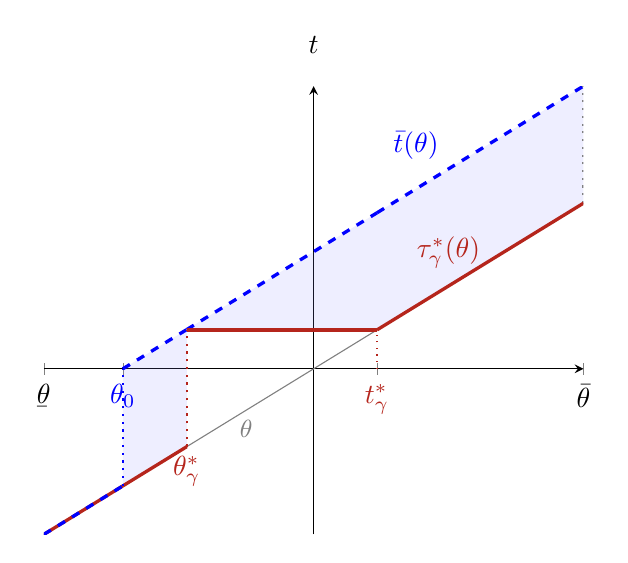
\begin{tikzpicture}
  \begin{axis}[axis x line=middle,
  axis y line=middle,
  xtick={-2,-1.414,0,0.47,2},
  xticklabels={$\ubar{\theta}$,$\mathcolor{Blue}{\theta_{0}}$,$0$,$\mathcolor{BrickRed}{t^{*}_{\gamma}}$,$\bar{\theta}$},
  ytick=\empty,
  yticklabels={},
  every axis x label/.style={
  		at={(ticklabel* cs:1.05)},
  		anchor=west,
  		},
  		every axis y label/.style={
  		at={(ticklabel* cs:1.05)},
  		anchor=south,
  		},
  	domain=-2:2,
  	samples=100,
  	xlabel={},
  	ylabel={$t$},
  	legend cell align=left,
  	legend pos=outer north east]
  \node[no marks, gray,below] at (axis cs:-0.5, -0.5) {\small$\theta$};
  \node[no marks,Blue,dashed,above left] at (axis cs:1, 2.414) {$\bar{t}(\theta)$};
  \addplot[smooth,gray,domain=-2:2] {x};
  \addplot[name path=A,smooth,very thick,dashed,Blue,domain=-1.414:-0.94] {x+1.414213};
  \addplot[name path=B,smooth,very thick,dashed,Blue,domain=-0.94:0.47] {x+1.414213};
  \addplot[name path=C,smooth,very thick,dashed,Blue,domain=0.47:2] {x+1.414213};
  \addplot[smooth,dotted,gray,thick]coordinates{(2,2)(2,3.414213)};
  \addplot[smooth,very thick,BrickRed,domain=-2:-1.414] {x};
  \addplot[name path=D,smooth,very thick,BrickRed,domain=-1.414:-0.94] {x};
  \addplot[smooth,very thick,Blue,dashed,domain=-2:-1.414] {x};
  \addplot[name path=E,smooth,very thick,BrickRed,domain=-0.94:0.47] {0.47};
  \addplot[BrickRed,thick,dotted] coordinates{(-0.94,-0.94) (-0.94,0.47)};
  \addplot[Blue,thick,dotted] coordinates{(-1.414,-1.414) (-1.414,0)};
  \node[no marks,Blue,below] at (axis cs:-0.94,-0.94) {$\mathcolor{BrickRed}{\theta^{*}_{\gamma}}$};
  \addplot[BrickRed,dotted] coordinates{(0.47,0) (0.47,0.47)};
  \addplot[name path=F,smooth,very thick,BrickRed,domain=0.47:2] {x};
  \node[no marks,BrickRed,above] at (axis cs:1,1.1) {$\tau_{\gamma}^{*}(\theta)$};
  \addplot[Blue!45,fill opacity=0.15] fill between[of=A and D];
  \addplot[Blue!45,fill opacity=0.15] fill between[of=B and E];
  \addplot[Blue!45,fill opacity=0.15] fill between[of=C and F];
  \end{axis}
\end{tikzpicture}
\caption{First-best (dashed lines) vs. second-best investment rule (plain lines)}
\label{fig:first_best}
\end{figure}

\paragraph{Comparative statics}

We first establish a preliminary result. We prove that if the distribution of types is sufficiently decreasing, then the optimal allocation cutoff never exceeds the highest initial type whatever the magnitude of investment costs.
\begin{lemma}\label{thm:suff_cond_low_threshold}
    If $f(\ubar{\theta})>1/\bar{\theta}$, then the optimal cutoff $t^{*}_{\gamma}$ belongs to the interval $\mathopen[0,\bar{\theta}\mathclose]$ for any $\gamma>0$.
\end{lemma}
\begin{proof}
    See \cref{secap:suff_cond_low_threshold}.
\end{proof}
The condition $f(\ubar{\theta})>1/\bar{\theta}$ ensures that a sufficiently high mass of agents is concentrated at the bottom of the type distribution and thus guarantees that $t^{*}_{\gamma}$ is bounded above by $\bar{\theta}$ for any $\gamma>0$. The reason for this is that the mass effect always dominates the incentive effect for the designer when the type distribution is very decreasing. In other words, fixing a threshold of approval higher than $\bar{\theta}$ would always exclude a too large mass of low type agents compared to the gain in terms of type investment at the cutoff $t^{*}_{\gamma}$.

We conduct the comparative statics exercise under the assumption that $f(\ubar{\theta})\geq 1/\bar{\theta}$ in the main text. This assumption is made for readability and our results could easily be extended when it is not satisfied. The designer's optimal expected payoff is given by
\begin{equation*}
	V^{*}_{\gamma}=t^{*}_{\gamma}\big(F(t^{*}_{\gamma})-F(\theta_{\gamma}^{*})\big)+\displaystyle\int_{t^{*}_{\gamma}}^{\bar{\theta}}\theta f(\theta) \, \mathrm{d}\theta
\end{equation*}
Moreover, the agents' interim optimal payoff is given by:
\begin{equation*}
	U_{\gamma}^{*}(\theta)=\left\{
	\begin{array}{ll}
	0	& \quad \text{if $\theta\in\mathopen[\ubar{\theta},\theta_{\gamma}^{*}\mathclose[$}\\
	1-\gamma c(t^{*}_{\gamma},\theta)	& \quad \text{if $\theta\in\mathopen[\theta_{\gamma}^{*},t^{*}_{\gamma}\mathclose[$} \\
	1	& \quad \text{if $\theta\in\mathopen[t^{*}_{\gamma},\bar{\theta}\mathclose]$}
	\end{array}
	\right..
\end{equation*}
First, we show that the designer's optimal allocation cutoff becomes looser as the investment costs increase.
\begin{proposition}\label{thm:comp_stat_threshold}
The optimal cutoff $t^{*}_{\gamma}$ defined in \cref{thm:pass_fail_opt} is monotonically decreasing towards zero as $\gamma$ increases, while the minimal initial type being admitted $\theta_{\gamma}^{*}$ is monotonically increasing towards zero as $\gamma$ increases. Moreover, the cutoffs $t^{*}_{\gamma}$ and $\theta_{\gamma}^{*}$ are both converging to zero as $\gamma$ tends to infinity.
\end{proposition}
\begin{proof}
    See \cref{secap:comp_stat_threshold}.
\end{proof}
The insight for \cref{thm:comp_stat_threshold} is as follows. Under the optimal mechanism, the agents with initial type $\theta^{*}_{\gamma}$ are indifferent between being rejected and keeping their initial type at cost $\gamma c(\theta^{*}_{\gamma},\theta^{*}_{\gamma})=0$, or investing in a the final type type $t^{*}_{\gamma}$ at a cost $\gamma c(t^{*}_{\gamma},\theta^{*}_{\gamma})=1$. Increasing the magnitude of the investment cost $\gamma$ has the effect of increasing the marginal type $\theta^{*}_{\gamma}$ thereby excluding a larger mass of agents with low initial types. The optimal response of the designer to mitigate this reduction in the mass of approved agents at the bottom is to lower the admission threshold to restore higher investment incentives for those agents. \Cref{thm:comp_stat_threshold} has the following direct consequence: When the cost of investment becomes arbitrarily large for all agents, the optimal mechanism is for no agent to invest in a new type and for the designer to approve only positive initial types.
\begin{corollary}[Asymptotics]\label{thm:asymptotics}
	The optimal experiment and optimal outcome respectively converges to $\mathds{1}\{t\geq0\}$ and to $\mathds{1}\{\theta\geq0\}$ as $\gamma\to +\infty$. Accordingly, the optimal payoffs converge to:
	\begin{equation*}
	    V^{*}_{\gamma} \underset{\gamma\to+\infty}{\longrightarrow}\int_{0}^{\bar{\theta}} \theta f(\theta) \, \mathrm{d}\theta,
	\end{equation*}
	and:
	\begin{equation*}
		U^{*}_{\gamma} \underset{\gamma\to+\infty}{\longrightarrow} 1-F(0).
	\end{equation*}
\end{corollary}
\Cref{thm:asymptotics} confirms that when the investment cost becomes infinitely large for all agents, the optimal mechanism is the one that would be optimal if the designer could only use an approval rule, that is, if he solved the following problem:
\begin{equation*}
    \max_{\sigma\colon\Theta\to\mathopen[0,1\mathclose]} \; \int_{\ubar{\theta}}^{\bar{\theta}} \theta \, \sigma(\theta) f(\theta) \, \mathrm{d}\theta.
\end{equation*}
\Cref{thm:comp_stat_threshold} allows us to derive comparative statics on the designer's welfare as well as on the agents' welfare when $\gamma$ increases.
\begin{proposition}[Comparative statics]\label{thm:comp_stat_welfare}
    Under the optimal mechanism $(\sigma^{*}_{\gamma},\tau^{*}_{\gamma})$ the following claims are satisfied:
    \begin{enumerate}[(i)]
        \item The designer's welfare $V^{*}_{\gamma}$ is decreasing in $\gamma$.
        \item There exists a cutoff $\tilde{\theta}_{\gamma}\in\mathopen]\theta^{*}_{\gamma},t^{*}_{\gamma}\mathclose[$ such that the interim welfare of agents $U^{*}_{\gamma}(\theta)$ is decreasing for all  $\theta\in\mathopen[\theta^{*}_{\gamma},\tilde{\theta}_{\gamma}]$ and increasing for all $\theta\in\mathopen[\tilde{\theta}_{\gamma},t^{*}_{\gamma}]$.
    \end{enumerate}
\end{proposition}
Quite naturally, \cref{thm:comp_stat_welfare} establishes that the designer's payoff decreases as the investment becomes costlier. First, the allocation cutoff decreases as $\gamma$ increases, which implies that agents who bunch at the threshold invest in a lower final type type in equilibrium. Moreover, the minimal type being approved $\theta^{*}_{\gamma}$ increases as $\gamma$ grows. Hence, the total mass of agents being approved under the optimal mechanism decreases as the cost of investment grows. Both effects lower the optimal payoff of the designer.

An upward scaling in the investment cost, however, has a non monotone effect on the agents' interim payoff. Indeed, the change in the agents' interim welfare due to a marginal increase in the investment cost can be decomposed in two effects which go in opposite directions. First, the direct effect of an increase in $\gamma$ is to scale up the cost of investment for all types. Second, the indirect effect of an increase in $\gamma$ is to lower the admission standard $t^{*}_{\gamma}$ which decreases the distance from any $\theta$ to the allocation cutoff $t^{*}_{\gamma}$. This decreases the cost of investment for all agents. \Cref{thm:comp_stat_welfare} shows that there exists a type threshold $\tilde{\theta}_{\gamma}$ above which all agents are gaining from an increase in $\gamma$ and below which all types are losing. The reason is that the indirect effect is stronger than the direct effect for all types which are sufficiently close to the allocation cutoff $t^{*}_{\gamma}$.

Comparative statics with respect to the welfare of agents turns out to be more intricate. Formally, the agents' aggregate welfare is given by:
\begin{equation*}
	U^{*}_{\gamma}=\underbrace{1-F(\theta^{*}_{\gamma})}_{\text{\shortstack{ex-ante allocation \\ probability}}}-\underbrace{\gamma\int_{\theta_{\gamma}^{*}}^{t^{*}_{\gamma}}c(t^{*}_{\gamma},\theta) f(\theta) \, \mathrm{d}\theta}_{\text{\shortstack{aggregate investment cost}}}.
\end{equation*}
The effect of $\gamma$ on agents' welfare is ambiguous. The direct effect of an increase in $\gamma$ is also to scale up the investment cost for all types of agents. Increasing $\gamma$ also makes $\theta_{\gamma}^{*}$ increase, so the ex-ante allocation probability is decreasing. However, an increase in $\gamma$ also decreases the allocation cutoff $t^{*}_{\gamma}$. This decreases the ex-ante probability of incurring the cost for agents at the top, and decreases the cost from investing to the cutoff for bunching agents. Depending on which of the effects dominate, the welfare of agents might increase or decrease. This suggests that the welfare of agents is not monotonic as a function of the magnitude of the investment costs.

\section{Proof of theorem \ref{thm:optimality_pass_fail}}\label{sec:proof_main_theorem}

In this section we state the main steps of the proof for \cref{thm:optimality_pass_fail}. Additional proofs can be found in \cref{secap:sol_variational_problem}. We first investigate the consequences of the monotonicity constraint imposed by \cref{thm:monotone_pol} for implementable investment rules. Next, we provide a characterization of incentive-compatible mechanisms in terms of a transformation of the agents' indirect utility function that we call the pseudo-utility function. Thanks to this characterization, we show that the problem of the designer can be restated as a problem of calculus of variations where the optimization variable is the agents' pseudo-utility function. We prove that the objective functional of this variational program is an upper-semicontinuous convex functional on a compact and convex set. As a result, there must exist some extreme point of the domain that is a solution of the designer's problem. We provide necessary conditions on the shape of these extreme points, which, together with the tangent inequality for convex functionals, allows us to establish the optimality of the pass-fail selection rules.

\paragraph{Admissible mechanisms: definition}

\Cref{thm:monotone_pol} sharpens the set of the investment rules that can be implemented by the designer. When the selection rule is monotone, no agent ever invests in a type that is strictly lower than its initial type, since this could only decrease its allocation probability. Therefore, we must have $\tau(\theta)\geq \theta$ for any $\theta\in\Theta$. We now show that there also exists an upper bound on agents' investments. Let us define $\bar{t}(\theta)=\max\{t\in T \, | \, \gamma c(t,\theta)\leq 1\}$. The type $\bar{t}(\theta)$ corresponds to the maximal type an agent with initial type $\theta$ would be willing to invest in, if he were allocated the good for sure. Since $c(\cdot,\theta)$ is a continuous and non-decreasing function over $T$ for any $\theta\in\Theta$, the upper bound $\bar{t}(\theta)$ is defined implicitly by the following equation of $t$:
\begin{equation}
	\label{eqn:Higher_Bound}
	\gamma c(t,\theta)=1, \tag{UB}
\end{equation}
which has a closed-form solution given by $\bar{t}(\theta)=\theta+\sqrt{2/\gamma}$ for any $\theta\in\Theta$. Hence, we always have $\theta\leq\tau(\theta)\leq\bar{t}(\theta)$ for all $\theta\in\Theta$ and we can normalize $T$ to $\mathopen[\ubar{\theta},\bar{t}(\bar{\theta})\mathclose]$ without loss of generality.

Any monotone selection rule must also induce agents approved with non-zero probability to acquire a non-negative final type. Let $\sigma$ be a monotone selection rule and let $t^{\dagger}$ be the lowest final type type guaranteeing a strictly positive approval probability to the agents under $\sigma$, i.e.:
\begin{equation*}
    t^{\dagger}=\min\left\{t\in T \, | \, \sigma(t)>0\right\}.
\end{equation*}
Since $\sigma$ is monotone, $t^{\dagger}$ must be non-negative. Let $\theta^{\dagger}$ be the initial type defined as the solution to the following equation of $\theta$:
\begin{equation*}
    \sigma(t^{\dagger})=\gamma c(t^{\dagger},\theta).
\end{equation*}
Denoting $\sigma(t^{\dagger})$ by $\sigma^{\dagger}$, we obtain:
\begin{equation*}
    \theta^{\dagger}=t^{\dagger}-\sqrt{\frac{2\sigma^{\dagger}}{\gamma}}.
\end{equation*}
Clearly, $\theta^{\dagger}$ corresponds to the lowest type investing in a non-zero final type under the selection rule $\sigma$. In particular, an agent with type $\theta^{\dagger}$ is always indifferent between keeping type $\theta^{\dagger}$ and acquiring final type $t^{\dagger}$. Hence, we always have $\tau(\theta)=\theta$ for all $\theta\in\mathopen[\theta_{0},\theta^{\dagger}\mathclose[$ and $\tau(\theta)\geq t^{\dagger}\geq 0$ for all $\theta\in\mathopen[\theta^{\dagger},\bar{\theta}\mathclose]$. Remark that, differently from $\theta_{0}$, the cutoff $\theta^{\dagger}$, together with the probability $\sigma^{\dagger}$, are part of the design and thus endogenous.

Third, let $(\sigma,\tau)$ be a mechanism such that $\sigma$ is monotone and assume that there exists a type $\theta$ such that $\tau(\theta)=\bar{t}(\theta)$. Since $\tau$ satisfies \labelcref{eqn:incentive_compatibility}, it must be non-decreasing by Topkis' theorem. Therefore, there must exist a type $\tilde{\theta}\in\Theta$ such that $\tilde{\theta}=\min\{\theta\in\Theta \, | \, \tau(\theta)=\bar{t}(\theta)\}$. The condition \labelcref{eqn:Higher_Bound} then implies that $\sigma(\bar{t}(\tilde{\theta}))=1$. Hence, since $\sigma$ is increasing and bounded above by 1, it must also be that $\sigma(t)=1$ for all $t\geq \bar{t}(\tilde{\theta})$. As a consequence, the final type $\bar{t}(\tilde{\theta})$ must be the smallest needed to pass with probability 1 under selection rule $\sigma$. Firstly, it might be the case that $\bar{t}(\tilde{\theta})<\bar{\theta}$. Then, since $\tau$ satisfies \labelcref{eqn:incentive_compatibility}, all agents born with types in the interval $\mathopen[\tilde{\theta},\bar{t}(\tilde{\theta})\mathclose[$ must invest exactly at the threshold $\bar{t}(\tilde{\theta})$ whereas all agents born with types in $\mathopen[\bar{t}(\tilde{\theta}),\bar{\theta}\mathclose]$ are already guaranteed to pass with probability 1 so $\tau(\theta)=\theta$ for all $\theta\geq \bar{t}(\tilde{\theta})$. Conversely, it might be the case that $\bar{t}(\tilde{\theta})\geq\bar{\theta}$. This means that no initial type is initially guaranteed to pass with certain probability under $\sigma$ and, again by \labelcref{eqn:incentive_compatibility}, all agents born with types in between $\mathopen[\tilde{\theta},\bar{\theta}\mathclose]$ must invest at $\bar{t}(\tilde{\theta})$. We sum up the previous discussion in the following corollary.
\begin{corollary}
\label{thm:monotone_pol_corollary}
If $\sigma$ satisfies properties (i) and (ii) from \cref{thm:monotone_pol}, then:
\begin{enumerate}[(i)]
	\item $\theta\leq\tau(\theta)\leq \bar{t}(\theta)$ for all $\theta\in \mathopen[\theta_{0},\bar{\theta}\mathclose]$;
	\item there always exists $\theta^{\dagger}\in\mathopen[\theta_{0},\bar{\theta}]$ such that $\tau(\theta)=\theta$ for all $\theta\in\mathopen[\theta_{0},\theta^{\dagger}\mathclose[$ and $\tau(\theta)\geq 0$ for all $\theta\in\mathopen[\theta^{\dagger},\bar{\theta}\mathclose]$, and;
	\item if there exists $\tilde{\theta}\in\mathopen[\theta_{0},\bar{\theta}\mathclose]$ such that $\tau(\tilde{\theta})=\bar{t}(\tilde{\theta})$ then we have the following:
	\begin{enumerate}[(a)]
		\item if $\bar{t}(\tilde{\theta})<\bar{\theta}$, then $\tau(\theta)=\bar{t}(\tilde{\theta})$ for all $\theta\in\mathopen[\tilde{\theta},\bar{t}(\tilde{\theta})\mathclose[$ and $\tau(\theta)=\theta$ for all $\theta\in\mathopen[\bar{t}(\tilde{\theta}), \bar{\theta}\mathclose]$;
		\item if $\bar{t}(\tilde{\theta})\geq\bar{\theta}$, then $\tau(\theta)=\bar{t}(\tilde{\theta})$ for all $\theta\in\mathopen[\bar{t}(\tilde{\theta}),\bar{\theta}\mathclose]$.
	\end{enumerate}
\end{enumerate}
\end{corollary}
Accordingly, we say that any mechanism $(\sigma,\tau)$ satisfying \labelcref{eqn:incentive_compatibility} as well as all properties from \cref{thm:monotone_pol} and \cref{thm:monotone_pol_corollary} is \emph{admissible}.

\paragraph{Admissible mechanisms: characterization}

The indirect utility of an agent of type $\theta$ under some selection rule $\sigma$ is given by
\begin{equation*}
	U(\theta)=\max_{t\in T} \; \sigma(t)-\gamma c(t,\theta).
\end{equation*}
Given the quadratic form of the cost function, simple algebra on the agents' objective function reveals that
\begin{equation*}
	 U(\theta)=\gamma\left(\max_{t\in T} \left\{ t\theta-\left(\frac{t^2}{2}-\frac{\sigma(t)}{\gamma}\right)\right\}-\frac{\theta^2}{2}\right).
\end{equation*}
Accordingly, we say that the value function defined by
\begin{equation*}
	u(\theta)=\max_{t\in T} \; t\theta-\left(\frac{t^2}{2}-\frac{\sigma(t)}{\gamma}\right),
\end{equation*}
is the agent's \emph{pseudo-utility} function under the rule $\sigma$. Let $\ubar{u}$ be the pseudo-utility function induced by the selection rule $\ubar{\sigma}(t)=0$ and $\bar{u}$ be the pseudo-utility function induced by the selection rule $\bar{\sigma}(t)=\mathds{1}\{t\geq0\}$.\footnote{Remark that $\ubar{\sigma}$ and $\bar{\sigma}$ are respectively the lowest and greatest recommendation rules in the class of monotone selection rules.} We have:
\begin{equation*}
	\ubar{u}(\theta)=\frac{\theta^2}{2}
\end{equation*}
and
\begin{equation*}
	\bar{u}(\theta)=\left\{\begin{array}{ll}
		\displaystyle\frac{1}{\gamma} & \text{if $\theta\in\mathopen[\theta_{0},0\mathclose[$} \\
		\displaystyle\frac{1}{\gamma}+\displaystyle\frac{\theta^2}{2} & \text{if $\theta\in\mathopen[0,\bar{\theta}\mathclose]$}
\end{array}
\right..
\end{equation*}
The next proposition characterizes admissible mechanisms in terms of properties of the pairs $(u,\tau)$.
\begin{lemma}\label{thm:charac_IC}
A mechanism $(\sigma,\tau)$ is admissible if, and only if, the pseudo-utility function $u$ and investment $\tau$ induced by $\sigma$ satisfy the following properties:
	\begin{enumerate}[(i)]
		\item $u$ is a convex function over $\mathopen[\theta_{0},\bar{\theta}]$ and is hence differentiable almost everywhere in that interval. Moreover, the envelope formula $u'(\theta)=\tau(\theta)$
		must hold at all points where $u$ is differentiable;
		\item $\ubar{u}(\theta)\leq u(\theta) \leq \bar{u}(\theta)$, for all $\theta\in\mathopen[\theta_{0},\bar{\theta}\mathclose]$;
		\item $\theta\leq u'(\theta)\leq \bar{t}(\theta)$ for almost all $\theta\in\mathopen[\theta_{0},\bar{\theta}\mathclose]$;
		\item $u(\theta)+u'(\theta)^2/2-\theta u'(\theta)\leq 1/\gamma$ for almost all $\theta\in\mathopen[\theta_{0},\bar{\theta}\mathclose]$;
		\item There always exists $\theta^{\dagger}\in\mathopen[\theta_{0},\bar{\theta}]$ such that $u(\theta)=\ubar{u}(\theta)$ for all $\theta\in\mathopen[\theta_{0},\theta^{\dagger}\mathclose]$ and $u$ is increasing and strictly above $\ubar{u}(\theta)$ for all $\theta\in\mathopen]\theta^{\dagger},\bar{\theta}\mathclose]$;
        \item If there exists $\hat{\theta}\in\mathopen[\theta_{0},\bar{\theta}\mathclose]$ such that $u'(\hat{\theta})=\bar{t}(\hat{\theta})$, then, if $\bar{t}(\hat{\theta})<\bar{\theta}$ we must have:
	    \begin{equation*}
		u(\theta)=\left\{
			\begin{array}{l l}
			\ubar{u}(\theta) & \text{if $\theta\in\mathopen[\theta_{0},\hat{\theta}\mathclose[$} \\
			\ubar{u}(\hat{\theta})+\bar{t}(\hat{\theta})(\theta-\hat{\theta}) & \text{if $\theta\in\mathopen[\hat{\theta},\bar{t}(\hat{\theta})\mathclose]$} \\
			\bar{u}(\theta) & \text{if $\theta\in\mathopen]\bar{t}(\hat{\theta}),\bar{\theta}\mathclose]$}
			\end{array}
		\right.,
	    \end{equation*}
        and if $\bar{t}(\hat{\theta})\geq\bar{\theta}$ then:
        \begin{equation*}
        u(\theta)=\left\{\begin{array}{ll}
        \ubar{u}(\theta) & \text{if $\theta\in\mathopen[\theta_{0},\hat{\theta}\mathclose[$} \\
        u(\theta)=\ubar{u}(\hat{\theta})+\bar{t}(\hat{\theta})(\theta-\hat{\theta}) & \text{if $\theta\in\mathopen[\hat{\theta},\bar{\theta}\mathclose]$}
        \end{array}
        \right.
	\end{equation*}
	\end{enumerate}
\end{lemma}
\begin{proof}
  See \cref{secap:charac_IC_proof}
\end{proof}
Property (i) is a consequence of Proposition 2 in \cite{Rochet1987} and ensures that the pair $(u,\tau)$ is consistent with the first-order conditions of the agents' optimization program wherever $\sigma$ is differentiable.\footnote{We know that, as a non-decreasing function, $\sigma$ must be differentiable on $T$ except maybe on a countable subset of points.} By the envelope formula, the function $u'$ is non-decreasing, hence the function $u$ must be convex. Another way to see why $u$ must be convex is the following fact. If we let $\varphi(t)=t^2/2-\sigma(t)/\gamma$, then:
\begin{equation*}
	u(\theta)=\max_{t\in T} \; \theta t-\varphi(t).
\end{equation*}
The function $u$ thus corresponds to the Legendre-Fenchel transform of the function $\varphi$, which is convex by definition. The previous expression also highlights the fact that $u$ corresponds to the indirect utility an agent with quasilinear payoff would get in a monopolistic screening problem \citep{Mussa1978} under some tariff $\varphi$.  Note, however, that unlike standard screening problems, the function $\varphi$ must be bounded between $\ubar{\varphi}(t)=t^2/2-\ubar{\sigma}(t)/\gamma$ and $\bar{\varphi}(t)=t^2/2-\bar{\sigma}(t)/\gamma$ because of the probability constraint on $\sigma$ and of \cref{thm:monotone_pol}. This implies property (ii). Property (iii), in turn, is simply the translation in terms of the pseudo-utility function of \cref{thm:monotone_pol_corollary}. Let us now explain property (iv). For this, we remind first that the \emph{outcome} $x\colon\mathopen[\theta_{0},\bar{\theta}]\to \mathopen[0,1\mathclose]$ of the selection rule $\sigma$ is given by $x(\theta)=\sigma(\tau(\theta))$ for all $\theta\in\mathopen[\theta_{0},\bar{\theta}]$. Using property (i), we can rewrite the outcome as a function of $u$ and $u'$ by substituting $\tau(\theta)$ by $u'(\theta)$ almost everywhere. Indeed, remembering that $U(\theta)=\gamma(u(\theta)-\theta^2/2)$ and remarking that $\sigma(\tau(\theta))=U(\theta)+\gamma c(\tau(\theta),\theta)$ we obtain:
\begin{equation*}
	 x(\theta)=\gamma\left(u(\theta)+\frac{u'(\theta)^2}{2}-\theta u'(\theta)\right),
\end{equation*}
for almost every $\theta\in \mathopen[\theta_{0},\bar{\theta}\mathclose]$. Thus, property (iv) expresses the fact that $x$ must be bounded above by 1. Importantly, it is easy to show that for any $u$ satisfying properties (ii) and (iii), we have $x(\theta)\geq 0$ almost everywhere. Nevertheless, we need to add property (iv) in the characterization as there exists some functions satisfying (ii) and (iii) such that $x(\theta)>1$ for some $\theta$ in $\mathopen[\theta_{0},\bar{\theta}]$. Finally, properties (v) and (vi) are direct consequences of \cref{thm:monotone_pol_corollary}.

\paragraph{Variational program}

Using the previous characterization, we can first define the following set.
\begin{definition}
The \emph{feasible set} of pseudo-utility functions is defined by:
\begin{equation*}
\mathcal{U}=\left\{u\colon\mathopen[\theta_{0},\bar{\theta}\mathclose]\to\mathbb{R}\, \middle| \, \text{$u$ satisfies properties (ii) to (vi) from \cref{thm:charac_IC}} \right\}.
\end{equation*}
\end{definition}
Any $u\in\mathcal{U}$ can be generated by some admissible mechanism $(\sigma,\tau)$ and any admissible mechanism $(\sigma,\tau)$ induces some pseudo-utility $u\in\mathcal{U}$. We thus refer to any $u\in\mathcal{U}$ as an admissible pseudo-utility. For the purpose of illustration, an instance of admissible pseudo-utility $u\in\mathcal{U}$ is depicted on \cref{fig:adm_psutility} while its induced investment rule, given by its derivative, is depicted on \cref{fig:induced_invest}.
\begin{figure}
  \centering
  \begin{subfigure}[t]{0.495\textwidth}
  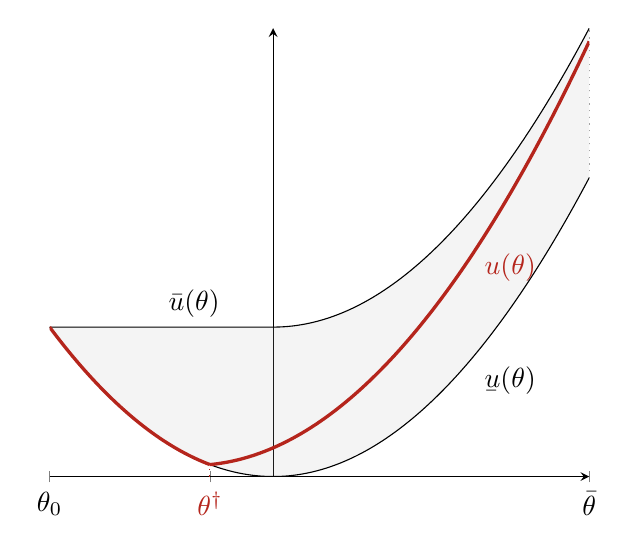
\begin{tikzpicture}
    \begin{axis}[
    axis x line=middle,
    axis y line=middle,
    xtick={-sqrt(2),-0.4,0,2},
	xticklabels={$\theta_{0}$,$\mathcolor{BrickRed}{\theta^{\dagger}}$,$0$,$\bar{\theta}$},
	ytick={0},
	yticklabels={$0$},
	every axis x label/.style={
	at={(ticklabel* cs:1.05)},
	anchor=west,
	},
    every axis y label/.style={
    at={(ticklabel* cs:1.05)},
    anchor=south,
    },
    domain=-1.414:2,
    samples=100,
    %xlabel={},
    %ylabel={},
    legend cell align=left,
    legend pos=outer north east]
    \addplot[name path=A,smooth,Black,domain=-1.414:2] {x^2/2};
    \node[no marks,Black,above] at (axis cs:-0.5, 1) {$\bar{u}(\theta)$};
    \addplot[name path=B,smooth,Black,domain=-1.414:2] {(!(x<-1.414) && (x<0))* 1 + (!(x<0) && (x<2))*(1+x^2/2)};
    \node[no marks,Black,below] at (axis cs:1.5, 0.8) {$\ubar{u}(\theta)$};
    \addplot[Black!30,fill opacity=0.15] fill between[of=A and B];
    \addplot[smooth,dotted,Black] coordinates{(2,2) (2,3)};
    \addplot[smooth,very thick,BrickRed,domain=-sqrt(2):-0.4] {x^2/2};
    \addplot[smooth,dotted,BrickRed] coordinates{(-0.4,0)(-0.4,0.08)};
    \addplot[smooth,very thick,BrickRed,domain=-0.4:2] {(-0.4)^2/2+0.1*(x+0.4)+0.9*(x+0.4)^2/2};
    \node[BrickRed,no marks] at (axis cs:1.5, 1.4) {$u(\theta)$};
	\end{axis}
  \end{tikzpicture}
  \caption{An admissible pseudo-utility $u$.}
\label{fig:adm_psutility}
\end{subfigure}
\begin{subfigure}[t]{0.495\textwidth}
	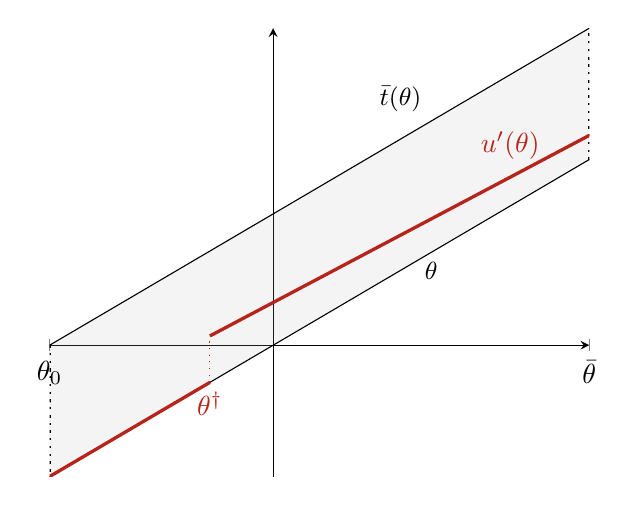
\begin{tikzpicture}
	\begin{axis}[axis x line=middle,
	axis y line=middle,
	xtick={-2,-1.414,0,2},
	xticklabels={$\ubar{\theta}$,$\theta_{0}$,$0$,$\bar{\theta}$},
	ytick=\empty,
	every axis x label/.style={
	at={(ticklabel* cs:1.05)},
	anchor=west,
	},
	every axis y label/.style={
	at={(ticklabel* cs:1.05)},
	anchor=south,
	},
	domain=-1.414:2,
	samples=100,
	%xlabel={},
	%ylabel={},
	legend cell align=left,
	legend pos=outer north east]
	\addplot[name path=A,smooth,Black,domain=-1.414:2] {x};
	\node[no marks,Black,below] at (axis cs:1, 1) {\small$\theta$};
	\node[BrickRed,no marks,below] at (axis cs:-0.4, -0.4) {$\theta^{\dagger}$};
	\addplot[name path=B,smooth,Black,domain=-1.414:2] {x+1.414213};
	\node[no marks,Black,above left] at (axis cs:1, 2.414) {\small$\bar{t}(\theta)$};
	\addplot[smooth,dotted,Black,thick]coordinates{(-1.414,0)(-1.414,-1.414)};
	\addplot[smooth,dotted,Black,thick]coordinates{(2,2)(2,3.414213)};
	\addplot[Black!30,fill opacity=0.15] fill between[of=A and B];
	\addplot[smooth,very thick,BrickRed,domain=-1.414:-0.4] {x};
	\addplot[smooth,dotted,BrickRed] coordinates{(-0.4,-0.4)(-0.4,0.1)};
	\addplot[smooth,very thick,BrickRed,domain=-0.4:2] {0.1+0.9*(x+0.4)};
	\node[BrickRed,no marks,above] at (axis cs:1.5, 1.9) {$u'(\theta)$};
	\end{axis}
\end{tikzpicture}
\caption{Its induced investment rule $u'$.}
\label{fig:induced_invest}
\end{subfigure}
\caption{An admissible pseudo-utility function $u\in\mathcal{U}$. Its induced investment rule is given by its derivative $u'$. Here $u(\theta)=0.45\times(\theta+0.4)^2+0.1\times(\theta+0.4)+0.08$.}
\end{figure}
Second, we can also rewrite the integrand of the designer's objective as a function of the agents' pseudo-utility by substituting $\tau(\theta)$ by $u'(\theta)$ and $\sigma(\tau(\theta))$ by $x(\theta)$ almost everywhere:
\begin{equation*}
	\tau(\theta) \, \sigma(\tau(\theta))=\gamma u'(\theta)\left(u(\theta)+\frac{u'(\theta)^2}{2}-\theta u'(\theta)\right),
\end{equation*}
for almost every $\theta\in \mathopen[\theta_{0},\bar{\theta}\mathclose]$. Therefore, for any pseudo-utility function $u\in\mathcal{U}$, the designer's payoff is given by:
\begin{equation*}
    V(u)=\int_{\theta_{0}}^{\bar{\theta}} \Lambda\big(\theta,u(\theta),u'(\theta)\big) \, \mathrm{d}\theta.
\end{equation*}
where, for any $\theta\in\mathopen[\theta_{0},\bar{\theta}]$, the function $\Lambda(\theta,\cdot,\cdot)$ is defined by
\begin{equation*}
    \Lambda(\theta,x,y)=\gamma y\left(x+\frac{y^2}{2}-\theta y\right)f(\theta)
\end{equation*}
for any $(x,y)\in\mathopen[\ubar{u}(\theta),\bar{u}(\theta)\mathclose]\times\mathopen[\theta,\bar{t}(\theta)\mathclose]$. The problem of the designer can therefore be expressed as the following problem of \emph{calculus of variations}\footnote{We refer to \cite{Clarke2013} for a thorough treatment of calculus of variations.}:
\begin{equation}\label{eqn:variational_pb}
	  \max_{u\in\mathcal{U}} \; \int_{\theta_{0}}^{\bar{\theta}} \Lambda\big(\theta,u(\theta),u'(\theta)\big) \, \mathrm{d}\theta \tag{V}
\end{equation}
Unfortunately, we cannot apply the standard resolution methods for program \labelcref{eqn:variational_pb} because the objective functional does not satisfy the necessary conditions to use the first-order approach \citep[see, for instance][Chapter 14, Section 1]{Clarke2013}. Therefore, we have to resort to different techniques to solve it.

\paragraph{Parameterization}

First of all, we parametrize the problem \labelcref{eqn:variational_pb} with respect to $\theta^{\dagger}$, the type whereupon the function $u$ starts taking-off with a non-negative slope from the lower bound $\ubar{u}$. Consider the following set of functions:
\begin{align*}
    \mathcal{U}(\theta^{\dagger})=\Big\{u\colon\mathopen[\theta^{\dagger},\bar{\theta}\mathclose]\to\mathbb{R}\, \big| \, &\text{$u$ is convex and increasing}, \\
    &\ubar{u}(\theta)\leq u(\theta)\leq\bar{u}(\theta), \\
    &\theta\leq u'(\theta)\leq\bar{t}(\theta), \\
    &u(\theta)+u'(\theta)^2/2-\theta u'(\theta)\leq 1/\gamma, \\
    &u(\theta^{\dagger})=\ubar{u}(\theta^{\dagger})\Big\}
\end{align*}
for any $\theta^{\dagger}\in\mathopen[\theta_{0},\bar{\theta}\mathclose]$. Remark that for any $u\in\mathcal{U}(\theta^{\dagger})$ we have $\Lambda(\theta,\ubar{u}(\theta),\ubar{u}'(\theta))=0$ for all $\theta\in\mathopen[\theta_{0},\theta^{\dagger}]$ and $\Lambda(\theta,u(\theta),u'(\theta))\geq 0$ for all $\theta\in\mathopen]\theta^{\dagger},\bar{\theta}]$. We can therefore always integrate the objective starting from $\theta^{\dagger}$. Accordingly, we define the parameterized objective functional $V_{\theta^{\dagger}}$ as follows:
\begin{equation*}
	V_{\theta^{\dagger}}(u)=\int_{\theta^{\dagger}}^{\bar{\theta}} \Lambda\big(\theta,u(\theta),u'(\theta)\big) \mathrm{d}\theta.
\end{equation*}


\paragraph{Restriction to extreme points of $\mathcal{U}(\theta^{\dagger})$}

We first prove the two following crucial observations.
\begin{lemma}\label{thm:compact_convex}
	For any $\theta^{\dagger}\in\mathopen[\theta_{0},\bar{\theta}]$, the set $\mathcal{U}(\theta^{\dagger})$ is convex and is compact with respect to the supremum-norm.
\end{lemma}
\begin{proof}
	See \cref{secap:compact_convex}.
\end{proof}
\begin{lemma}\label{thm:convexity_objective}
	For any $\theta^{\dagger}\in\mathopen[\theta^{\dagger},\bar{\theta}\mathclose]$, the functional $V_{\theta^{\dagger}}\colon\mathcal{U}(\theta^{\dagger})\to\mathbb{R}$ is \emph{upper semicontinuous}. Moreover, if \cref{thm:ddist} is satisfied, then it is also \emph{convex}.
\end{lemma}
\begin{proof}
    See \cref{secap:convexity_objective}.
\end{proof}
\Cref{thm:compact_convex,thm:convexity_objective} have the following implications: First, by the \emph{Krein–Milman theorem} \citep[][Theorem 7.68]{Aliprantis2006} it must be that the set $\mathcal{U}(\theta^{\dagger})$ is the closed, convex hull of its extreme points and, in particular, that the set $\mathcal{E}(\theta^{\dagger})$ of extreme points of $\mathcal{U}(\theta^{\dagger})$ is non-empty. Second, \emph{Bauer's Maximum Principle} \citep[][Theorem 7.69]{Aliprantis2006} ensures that the functional $V_{\theta^{\dagger}}$ must admit a maximizer which belongs to $\mathcal{E}(\theta^{\dagger})$.

A function $u\in\mathcal{U}(\theta^{\dagger})$ is an extreme point if there does not exist $u_1,u_2\in\mathcal{U}$ and $\alpha\in\mathopen]0,1\mathclose[$ such that $u=\alpha u_1+(1-\alpha)u_2$. We provide next an equivalent and more convenient definition of extreme points.
\begin{definition}
	Let $C$ be a compact and convex subset of a locally convex topological vector space $X$. A point $x\in C$ is an extreme point if, and only if, for every direction $h\in X$ such that $h\neq 0$, we either have that $x+h\notin C$ or $x-h\notin C$, or both.
\end{definition}
We proved in \cref{thm:compact_convex} that $\mathcal{U}(\theta^{\dagger})$ is a compact and convex subset of the normed linear space $(\mathcal{C}(\mathopen[\theta^{\dagger},\bar{\theta}\mathclose]),\lVert\cdot\rVert_{\infty})$. Therefore, a function $u$ belongs to $\mathcal{E}(\theta^{\dagger})$ if, and only if, there does not exist any direction $h\in\mathcal{C}(\mathopen[\theta^{\dagger},\bar{\theta}\mathclose])$ such that $u-h\in\mathcal{U}$ and $u+h\in\mathcal{U}$. In the next lemma, we provide necessary conditions on the extreme points of $\mathcal{U}(\theta^{\dagger})$.
\begin{lemma}\label{thm:nec_cond_ext_pt}
If $u\in\mathcal{U}(\theta^{\dagger})$ is an extreme point then:
\begin{enumerate}[(i)]
    \item $u$ must increasing and piecewise affine on the interval $\mathopen[\theta^{\dagger},0\mathclose]$, i.e., there exists a countable set $I$ and a sequence $(a_i,b_i)_{i\in I}$ such that $0 \leq a_{i}\leq a_{i+1}$ and $b_{i}\in\mathbb{R}$ for all $i\in I$, and that $u(\theta)=\max\{a_{i}\theta+b_{i} \, | \, i\in I, a_{0}\theta^{\dagger}+b_0=\ubar{u}(\theta^{\dagger})\}$ for all $\mathopen[\theta^{\dagger},0\mathclose[$;
    \item $u$ must be a convex connection between increasing affine and quadratic arcs on the interval $\mathopen]0,\bar{\theta}\mathclose]$, i.e., there exists a countable set $J$, a sequence $(c_{j})_{j\in J}$ such that $ u(0) \leq c_{j}\leq c_{j+1}\leq 1/\gamma$ for any $j\in J$, as well as a collection of intervals $(\mathopen[\ubar{x}_{j},\bar{x}_{j}\mathclose[)_{j\in J}$ such that $\mathopen[\ubar{x}_{j},\bar{x}_{j}\mathclose[\subseteq\mathopen]0,\bar{\theta}\mathclose]$, that $\bar{x}_{j}\leq \ubar{x}_{j+1}$ for all $j\in J$, and that $u(\theta)=\theta^2/2+c_j$ for every $j\in J$ and any $\theta\in \mathopen[\ubar{x}_{j},\bar{x}_{j}\mathclose[$. Moreover, whenever $\theta \in \mathopen]0,\bar{\theta}\mathclose]\setminus\cup_{j\in J}\mathopen[\ubar{x}_{j},\bar{x}_{j}\mathclose[$, $u$ must be increasing and piecewise affine, and must join two quadratic arcs while staying convex.
\end{enumerate}
\end{lemma}
\begin{proof}
    See \cref{secap:nec_cond_ext_pt}
\end{proof}
\Cref{thm:nec_cond_ext_pt} provides necessary conditions on the extreme points. It shows that if $u\in\mathcal{E}(\theta^{\dagger})$, then it must be the convex junction between increasing affine and quadratic arcs. An example of extreme point is depicted on \cref{fig:ext_pt} together with its derivative on \cref{fig:invest_ext_pt}.
\begin{figure}
  \centering
  \begin{subfigure}[t]{0.495\textwidth}
  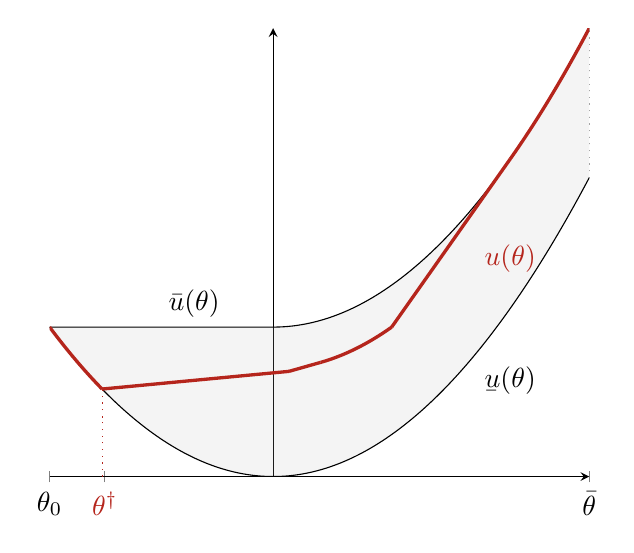
\begin{tikzpicture}
    \begin{axis}[
    axis x line=middle,
    axis y line=middle,
    xtick={-sqrt(2),-1.06512,0,2},
	xticklabels={$\theta_{0}$,$\mathcolor{BrickRed}{\theta^{\dagger}}$,$0$,$\bar{\theta}$},
	ytick={0},
	yticklabels={$0$},
	every axis x label/.style={
	at={(ticklabel* cs:1.05)},
	anchor=west,
	},
    every axis y label/.style={
    at={(ticklabel* cs:1.05)},
    anchor=south,
    },
    domain=-1.414:2,
    samples=100,
    %xlabel={},
    %ylabel={},
    legend cell align=left,
    legend pos=outer north east]
    \addplot[name path=A,smooth,Black,domain=-1.414:2] {x^2/2};
    \node[no marks,Black,above] at (axis cs:-0.5, 1) {$\bar{u}(\theta)$};
    \addplot[name path=B,smooth,Black,domain=-1.414:2] {(!(x<-1.414) && (x<0))* 1 + (!(x<0) && (x<2))*(1+x^2/2)};
    \node[no marks,Black,below] at (axis cs:1.5, 0.8) {$\ubar{u}(\theta)$};
    \addplot[Black!30,fill opacity=0.15] fill between[of=A and B];
    \addplot[smooth,dotted,Black] coordinates{(2,2) (2,3)};
    \addplot[smooth,very thick,BrickRed,domain=-sqrt(2):-1.08216] {x^2/2};
    \addplot[smooth,dotted,BrickRed] coordinates{(-1.08216,0)(-1.08216,0.5855351328)};
    \addplot[smooth,very thick,BrickRed,domain=-1.08216:0.1] {0.69375+0.1*x};
    \addplot[smooth,very thick,BrickRed,domain=0.1:0.3] {539/800+0.3*x};
    \addplot[smooth,very thick,BrickRed,domain=0.3:0.75] {23/32+x^2/2};
    \addplot[smooth,very thick,BrickRed,domain=0.75:1.5] {1.5*(x-1.5+sqrt(2))+(1.5-sqrt(2))^2/2};
    \addplot[smooth,very thick,BrickRed,domain=1.5:2] {1+x^2/2};
    \node[BrickRed,no marks,above] at (axis cs:1.5, 1.3) {$u(\theta)$};
	\end{axis}
  \end{tikzpicture}
  \caption{An extreme point $u$.}
\label{fig:ext_pt}
\end{subfigure}
\begin{subfigure}[t]{0.495\textwidth}
	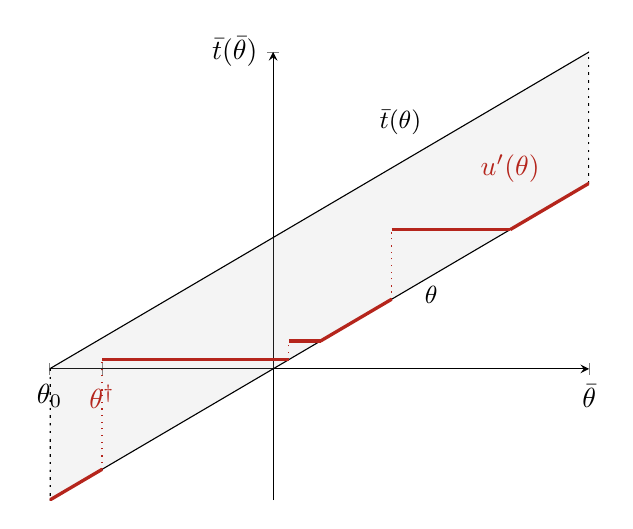
\begin{tikzpicture}
	\begin{axis}[axis x line=middle,
	axis y line=middle,
	xtick={-2,-1.414,-1.08216,0,2},
	xticklabels={$\ubar{\theta}$,$\theta_{0}$,$\mathcolor{BrickRed}{\theta^{\dagger}}$,$0$,$\bar{\theta}$},
	ytick={-2,3.414213},
	yticklabels={$\ubar{\theta}$,$\bar{t}(\bar{\theta})$},
	every axis x label/.style={
	at={(ticklabel* cs:1.05)},
	anchor=west,
	},
	every axis y label/.style={
	at={(ticklabel* cs:1.05)},
	anchor=south,
	},
	domain=-1.414:2,
	samples=100,
	%xlabel={},
	%ylabel={},
	legend cell align=left,
	legend pos=outer north east]
	\addplot[name path=A,smooth,Black,domain=-1.414:2] {x};
	\node[no marks,Black,below] at (axis cs:1, 1) {\small$\theta$};
	\addplot[name path=B,smooth,Black,domain=-1.414:2] {x+1.414213};
	\node[no marks,Black,above left] at (axis cs:1, 2.414) {\small$\bar{t}(\theta)$};
	\addplot[smooth,dotted,Black,thick]coordinates{(-1.414,0)(-1.414,-1.414)};
	\addplot[smooth,dotted,Black,thick]coordinates{(2,2)(2,3.414213)};
	\addplot[Black!30,fill opacity=0.15] fill between[of=A and B];
	\addplot[smooth,very thick,BrickRed,domain=-sqrt(2):-1.08216] {x};
    \addplot[smooth,dotted,BrickRed] coordinates{(-1.08216,-1.08216)(-1.08216,0.1)};
    \addplot[smooth,very thick,BrickRed,domain=-1.08216:0.1] {0.1};
    \addplot[smooth,dotted,BrickRed] coordinates{(0.1,0.1)(0.1,0.3)};
    \addplot[smooth,very thick,BrickRed,domain=0.1:0.3] {0.3};
    \addplot[smooth,very thick,BrickRed,domain=0.3:0.75] {x};
    \addplot[smooth,dotted,BrickRed] coordinates{(0.75,0.75)(0.75,1.5)};
    \addplot[smooth,very thick,BrickRed,domain=0.75:1.5] {1.5};
    \addplot[smooth,very thick,BrickRed,domain=1.5:2] {x};
	\node[BrickRed,no marks,above] at (axis cs:1.5, 1.9) {$u'(\theta)$};
	\end{axis}
\end{tikzpicture}
\caption{Its induced investment rule $u'$.}
\label{fig:invest_ext_pt}
\end{subfigure}
\caption{An extreme point $u\in\mathcal{E}(\theta^{\dagger})$ together with its induced investment rule $u'$.}
\end{figure}
The reason why extreme points take this particular form is that such curves either make the bounds on the derivative binding when $u$ is confounded with $\theta$ or $\bar{t}(\theta)$, or make the convexity constraint binding when $u'$ is flat, i.e., $u$ is affine. However, due to the constraint that $u'(\theta)\geq 0$, the function $u$ cannot be quadratic if $\theta<0$ because otherwise  one would have $u'(\theta)=\theta<0$.

\Cref{thm:nec_cond_ext_pt} has an important implication. When searching for an optimal solution of \labelcref{eqn:variational_pb}, one can restrict attention without loss of optimality to functions that are convex connections of linear and quadratic arcs. Let us define the function $u^{\dagger}$ given by:
\begin{equation*}
    u^{\dagger}(\theta)=\left\{\begin{array}{ll}
        \ubar{u}(\theta^{\dagger})+\bar{t}(\theta^{\dagger})(\theta-\theta^{\dagger}) & \text{if $\theta\in\mathopen[\theta^{\dagger},\bar{t}(\theta^{\dagger})\mathclose[$} \\
        \bar{u}(\theta) & \text{if $\theta\in\mathopen[\bar{t}(\theta^{\dagger}), \bar{\theta}\mathclose]$}
    \end{array}
    \right..
\end{equation*}
This function corresponds to the pseudo-utility function implemented by a $\bar{t}(\theta^{\dagger})$-pass-fail rule restricted to the interval $\mathopen[\theta^{\dagger},\bar{\theta}]$. Indeed, remember that \cref{thm:charac_IC} implies that $(u^{\dagger})'(\theta)$ corresponds to the optimal investment after the cutoff $\theta^{\dagger}$. It is easy to verify that:
\begin{equation}
		(u^{\dagger})'(\theta)=\left\{
		\begin{array}{l l}
			\bar{t}(\theta^{\dagger}) & \text{if $\theta\in\mathopen[\theta^{\dagger},\bar{t}(\theta^{\dagger})\mathclose[$} \\
			\theta & \text{if $\theta\in\mathopen[\bar{t}(\theta^{\dagger}),\bar{\theta}\mathclose]$}
		\end{array}
		\right.
\end{equation}
if $\theta^{\dagger}<\bar{\theta}-\sqrt{2/\gamma}$, and
\begin{equation}
    (u^{\dagger})'(\theta)=\bar{t}(\theta^{\dagger}),
\end{equation}
if $\theta^{\dagger}\geq\bar{\theta}-\sqrt{2/\gamma}$. This corresponds to the investment rule that would be implemented under a $\bar{t}(\theta^{\dagger})$-pass-fail rule. Importantly, the function $u^{\dagger}$ satisfies all the necessary conditions in \cref{thm:nec_cond_ext_pt} and is an extreme point of $\mathcal{U}(\theta^{\dagger})$. Also importantly, $u^{\dagger}$ bounds any other function $u\in\mathcal{U}(\theta^{\dagger})$ from above so $u^{\dagger}-u\geq0$ for any $u\in\mathcal{U}(\theta^{\dagger})$. The final step of our proof is to show that $u^{\dagger}$ is an optimal solution.

To do so, we first recall the following characterization of convex functionals.
\begin{lemma}[Above the tangent property for convex functions]\label{thm:above_tangent}
    Let $X$ be a normed space, $C$ be a non-empty closed convex subset of $X$ and $\varphi\colon C\to \mathbb{R}$ be a Gâteaux differentiable function, with Gâteaux derivative at $x\in C$ in direction $h\in X$ given by $\mathrm{D}\varphi(x)(h)$. Then, $\varphi$ is convex if, and only if:
    \begin{equation*}
        \varphi(y)\geq \varphi(x)+ \mathrm{D}\varphi(x)(y-x)
    \end{equation*}
    for all $(x,y)\in C\times C$.
\end{lemma}
By \cref{thm:compact_convex}, we know that the set $\mathcal{U}(\theta^{\dagger})$ is a compact and convex subset of the normed linear space $\mathopen(\mathcal{C}(\mathopen[\theta^{\dagger},\bar{\theta}\mathclose]\mathclose), \lVert\cdot\rVert_{\infty})$. Moreover, we also proved in \cref{thm:convexity_objective} that $V_{\theta^{\dagger}}$ is convex over $\mathcal{U}(\theta^{\dagger})$ under \cref{thm:ddist}. We now prove that the functional $V_{\theta^{\dagger}}$ is Gâteaux differentiable everywhere on $\mathcal{U}(\theta^{\dagger})$ and we give a closed form for its Gâteaux derivative.
\begin{lemma}\label{thm:gateaux_derivative}
The functional $V_{\theta^{\dagger}}$ is Gâteaux differentiable and has a Gâteaux derivative at $u$ in direction $h$ given by:
\begin{multline*}
    \mathrm{D} V_{\theta^{\dagger}}(u)(h)=\int_{\theta^{\dagger}}^{\bar{\theta}}\Bigg(-\left(\left(u(\theta)+\frac{1}{2} u'(\theta)^2 -\theta u'(\theta)\right) + u'(\theta)\left(u'(\theta)-\theta\right)\right) f'(\theta) \\
    +\Big(u'(\theta)-2 u''(\theta)\left(u'(\theta)-\theta\right)-u'(\theta)\left(u''(\theta)-1\right)\Big) f(\theta) \Bigg) h(\theta) \,  \mathrm{d}\theta.
\end{multline*}
\end{lemma}
\begin{proof}
    See \cref{secap:gateaux_derivative}.
\end{proof}
Hence, \cref{thm:above_tangent} and \cref{thm:gateaux_derivative} together imply that:
\begin{equation}\label{eqn:above_tangent}
    V_{\theta^{\dagger}}(v)\geq V_{\theta^{\dagger}}(u)+\mathrm{D} V_{\theta^{\dagger}}(u)(v-u)
\end{equation}
for any $(u,v)\in\mathcal{U}(\theta^{\dagger})\times \mathcal{U}(\theta^{\dagger})$ and any $\theta^{\dagger}\in\mathopen[\theta_{0},\bar{\theta}]$. In particular, \cref{eqn:above_tangent} must be satisfied when $v=u^{\dagger}$ and when $u$ is an extreme point, since $\mathcal{E}(\theta^{\dagger})\subset\mathcal{U}(\theta^{\dagger})$. That is:
\begin{equation}\label{eqn:above_tangent_ext}
    V_{\theta^{\dagger}}(u^{\dagger})\geq V_{\theta^{\dagger}}(u)+\mathrm{D} V_{\theta^{\dagger}}(u)(u^{\dagger}-u)
\end{equation}
for any $u\in\mathcal{E}(\theta^{\dagger})$. We now prove the following important result.
\begin{lemma}\label{thm:positive_deriv}
    If \cref{thm:ddist} is satisfied, then $\mathrm{D} V_{\theta^{\dagger}}(u)(u^{\dagger}-u)\geq 0$ for any $u\in\mathcal{E}(\theta^{\dagger})$.
\end{lemma}
\begin{proof}
    See \cref{secap:positive_deriv}.
\end{proof}
\Cref{thm:positive_deriv} is the final step of our proof. Indeed, \cref{eqn:above_tangent_ext,thm:positive_deriv} together entail that $V_{\theta^{\dagger}}(u^{\dagger})\geq V_{\theta^{\dagger}}(u)$ for any $u\in\mathcal{E}(\theta^{\dagger})$, proving the optimality of $u^{\dagger}$. The proof of \cref{thm:positive_deriv} relies on the fact that at any extreme point $u \in \mathcal{E}(\theta^{\dagger})$, we have either $u''(\theta)=0$ and $u'(\theta)=a$ for some constant $a>0$ on intervals where $u$ is linear, or $u''(\theta)=1$ and $u'(\theta)=\theta$ on intervals where $u$ is quadratic. This, together with the fact that $u^{\dagger}(\theta)-u(\theta)\geq 0$ for any $\theta \in\mathopen[\theta_{0},\bar{\theta}\mathclose]$ implies that the integrand in the expression of the Gâteaux derivative given in \cref{thm:gateaux_derivative} is always positive. Intuitively, this condition means that at a given cutoff $\theta^{\dagger}$, when we restrict to the extreme points of the domain $\mathcal{U}(\theta^{\dagger})$, deviating to the pseudo-utility $u^{\dagger}$ always locally increase the value of the principal's objective. Note that any extreme point $u \in \mathcal{E}(\theta^{\dagger})$ can be implemented by an increasing step selection rule. The linear parts of $u$ then correspond to regions where agents bunch at the next step and the quadratic parts correspond to regions where agents have an investment cost too large to reach the next step and therefore keep their type at zero cost. \Cref{thm:positive_deriv} therefore basically states that among all step selection rules, the best one is the one with two steps. A step with value zero and a step with value one, separated by the allocation cutoff $\bar{t}(\theta^{\dagger})$. Optimizing the designer's payoff over the one-dimensional parameter $\theta^{\dagger}$ ends the proof of \cref{thm:optimality_pass_fail}.

\section{Extensions}\label{sec:extensions}

We study three extensions of our model. First, we add a capacity constraint to the principal allocation problem. Second, we solve the problem of a utilitarian social planner. In both cases, the optimal selection rule remains pass-fail. Finally, we relax the principal's commitment power. Instead of committing to a mechanism, the principal bases her allocation decision on the information provided by an intermediary with aligned preferences. We show that the principal-optimal allocation can be implemented by the intermediary through information design.

\subsection{Capacity constrained designer}

In the baseline model, the designer possesses the same mass of resources than the total mass of agents. In this extension, we assume instead that the designer is \emph{capacity constrained}. That is, she can at most allocate a positive measure $\kappa<1$, of resources. Under that additional constraint, the problem of the designer writes as follows:
\begin{align*}
  \underset{\sigma,\tau}{\text{maximize}} \quad & \int_{\ubar{\theta}}^{\bar{\theta}} \tau(\theta) \, \sigma(\tau(\theta)) f(\theta) \, \mathrm{d}\theta \\
  \text{subject to} \quad & \tau(\theta)\in \underset{t\in T}{\arg\max} \; \sigma(t)-\gamma c(t,\theta) \tag{IC} \\
  \text{and} \quad & \int_{\ubar{\theta}}^{\bar{\theta}} \sigma(\tau(\theta)) f(\theta) \; \mathrm{d}\theta \leq \kappa \tag{C} \label{eqn:cap_constraint}
\end{align*}
Letting $\lambda\geq 0$ be the Lagrange multiplier on the constraint \labelcref{eqn:cap_constraint}, we can observe that the previous problem reduces to the same problem than \labelcref{eqn:designer_program} where the preference threshold of the designer has been moved from $0$ to $\lambda$:
\begin{align*}
  \underset{\sigma,\tau,\lambda}{\text{maximize}} \quad & \int_{\ubar{\theta}}^{\bar{\theta}} (\tau(\theta)-\lambda) \, \sigma(\tau(\theta)) f(\theta) \, \mathrm{d}\theta +\lambda\kappa \\
  \text{subject to} \quad & \tau(\theta)\in \underset{t\in T}{\arg\max} \; \sigma(t)-\gamma c(t,\theta) \tag{IC}
\end{align*}
Since the structure of the problem is unchanged, we can use the proof of \cref{thm:optimality_pass_fail} verbatim on the proviso that the designer restrict herself to selection rules that are zero below the preference threshold $\lambda$, and non-decreasing above. We thus have the following result.
\begin{proposition}\label{thm:optim_alloc_capacity}
   Pass-fail selection rules solve the capacity constrained allocation problem. Moreover, if the capacity constraint is binding, then the optimal threshold is tighter than under no capacity constraint.
\end{proposition}
This proposition follows from the standard Kuhn and Tucker method, and we therefore omit its proof. The idea is as follows. If the solution to the constrained program is the same as in the case when $\kappa=1$ then the multiplier $\lambda$ is null and the capacity constraint is not binding at the optimum. If the solution differs, then $\lambda>0$ and the capacity constraint kicks in. Whenever it is the case, the selection cutoff must, by definition, weakly increase compared to the unconstrained selection cutoff. Otherwise, it would mean that the designer allocates at least the same mass of resources than under the unconstrained program, a contradiction.

\subsection{Utilitarian welfare}

We now consider the problem of a utilitarian social planner seeking to maximize weighted social welfare. Formally, the planner's program writes as follows:
\begin{align*}
  \underset{\sigma,\tau}{\text{maximize}} \quad & \int_{\ubar{\theta}}^{\bar{\theta}} \tau(\theta) \, \sigma(\tau(\theta)) f(\theta) \, \mathrm{d}\theta +\alpha \int_{\ubar{\theta}}^{\bar{\theta}} \big(\sigma(\tau(\theta))-\gamma c(\tau(\theta),\theta) \big) f(\theta) \, \mathrm{d}\theta \\
  \text{subject to} \quad & \tau(\theta)\in \underset{t\in T}{\arg\max} \; \sigma(t)-\gamma c(t,\theta) \tag{IC}
\end{align*}
where $\alpha>0$ is the Pareto weight the planner assigns to the welfare of agents. When $\alpha<1$, the planner cares more about the welfare of the principal, and conversely when $\alpha>1$. We prove that the welfare-optimal selection rules are also deterministic, and have a smaller allocation threshold compared to the principal-optimal rule.
\begin{proposition}\label{thm:optimal_welfare}
   The welfare-optimal pass-fail rule solves the problem of the planner. Moreover, the welfare-optimal allocation cutoff is lower than under the optimal selection rule of the principal.
\end{proposition}
\begin{proof}
 See \cref{secap:optimal_welfare_proof}.
\end{proof}
\Cref{thm:optimal_welfare} states that taking into account the aggregate welfare of agents does not affect the deterministic structure of the optimal selection rule, and leads to less severe selection than under the principal-optimal selection rule. We illustrate the discrepancy between the welfare-optimal and the principal-optimal selection rules in \cref{fig:welfare_vs_principal}.
\begin{figure}
  \begin{subfigure}[t]{0.495\textwidth}
	\begin{tikzpicture}[scale=1]
	\begin{axis}[axis x line=middle,
	axis y line=middle,
	xtick={-0.9092,-0.1822,0.505,1.232},
	xticklabels={$\mathcolor{Blue}{\theta_{\gamma,\alpha}^{W}}$,$\mathcolor{BrickRed}{\theta_{\gamma}^{*}}$, $\mathcolor{Blue}{t_{\gamma,\alpha}^{W}}$,$\mathcolor{BrickRed}{t_{\gamma}^{*}}$},
	ytick={1},
	yticklabels={$1$},
	every axis x label/.style={
	at={(ticklabel* cs:1.05)},
	anchor=west,
	},
	every axis y label/.style={
	at={(ticklabel* cs:1.05)},
	anchor=south,
	},
	domain=-2:2,
	ymax=1.25,
	ymin=-0.1,
	samples=100,
	%xlabel={},
	%ylabel={},
	legend cell align=left,
	legend pos=outer north east]
	\addplot[smooth,very thick,BrickRed,domain=-2:1.232] {0};
	\addplot[smooth,very thick,BrickRed,domain=1.232:2] {1};
	\addplot[smooth,dotted,thick,BrickRed] coordinates{(1.232,0)(1.232,1)};
	\node[BrickRed,no marks] at (axis cs:1.232, 1) {$\bullet$};
	\node[BrickRed,no marks,above right] at (axis cs:1.232, 1) {$\sigma_{\gamma}^{*}(t)$};
	\addplot[smooth,very thick,Blue,dashed,domain=-2:0.505] {0};
	\addplot[smooth,very thick,Blue,dashed,domain=0.505:2] {1};
	\addplot[smooth,dotted,thick,Blue] coordinates{(0.505,0)(0.505,1)};
	\node[Blue,no marks] at (axis cs:0.505, 1) {$\bullet$};
	\node[Blue,no marks,above] at (axis cs:0.505, 1) {$\sigma_{\gamma,\alpha}^{W}(t)$};
	\end{axis}
\end{tikzpicture}
\caption{Optimal pass-fail selection rule.}
\label{fig:welfare_pass_fail}
\end{subfigure}
\begin{subfigure}[t]{0.495\textwidth}
	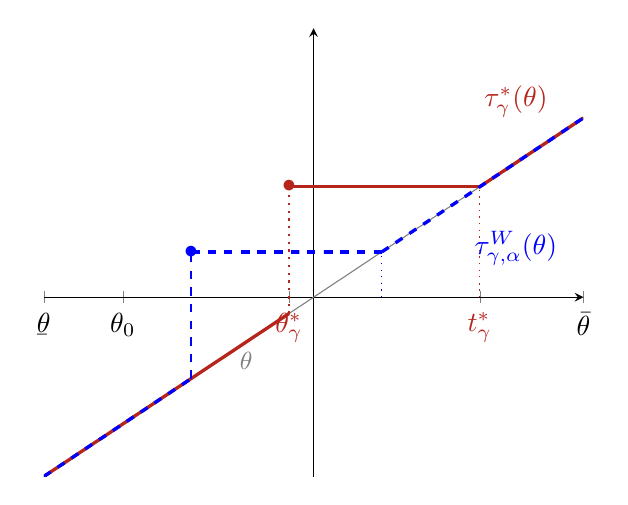
\begin{tikzpicture}[scale=1]
	\begin{axis}[axis x line=middle,
	axis y line=middle,
	xtick={-2,-sqrt(2),-0.1822,1.232,2},
	xticklabels={$\ubar{\theta}$,$\theta_{0}$,$\mathcolor{BrickRed}{\theta_{\gamma}^{*}}$,$\mathcolor{BrickRed}{t_{\gamma}^{*}}$,$\bar{\theta}$},
	ytick=\empty,
	every axis x label/.style={
	at={(ticklabel* cs:1.05)},
	anchor=west,
	},
	every axis y label/.style={
	at={(ticklabel* cs:1.05)},
	anchor=south,
	},
	domain=-2:2,
	samples=100,
	ymax=3,
	%xlabel={},
	%ylabel={},
	legend cell align=left,
	legend pos=outer north east]
	\node[no marks, gray,below] at (axis cs:-0.5, -0.5) {\small$\theta$};
	\addplot[smooth,gray,domain=-2:2] {x};
	\addplot[smooth,very thick,BrickRed,domain=-2:-0.1822] {x};
	\addplot[smooth,dotted,thick,BrickRed] coordinates{(-0.1822,-0.1822)(-0.1822,1.232)};
	\node[BrickRed,no marks] at (axis cs:-0.1822,1.232) {$\bullet$};
	\addplot[smooth,very thick,BrickRed,domain=-0.1822:1.232] {1.232};
	\addplot[smooth,dotted,BrickRed] coordinates{(1.232,0)(1.232,1.232)};
	\addplot[smooth,very thick,BrickRed,domain=1.232:2] {x};
	\node[BrickRed,no marks,above] at (axis cs:1.5, 1.9) {$\tau_{\gamma}^{*}(\theta)$};
	\addplot[smooth,very thick,Blue,dashed,domain=-2:-0.9092] {x};
	\addplot[smooth,dotted,thick,Blue,dashed] coordinates{(-0.9092,-0.9092)(-0.9092,0.505)};
	\node[Blue,dashed,no marks] at (axis cs:-0.9092,0.505) {$\bullet$};
	\addplot[smooth,very thick,Blue,dashed,domain=-0.9092:0.505] {0.505};
	\addplot[smooth,dotted,Blue] coordinates{(0.505,0)(0.505,0.505)};
	\addplot[smooth,very thick,Blue,dashed,domain=0.505:2] {x};
	\node[Blue,no marks,above] at (axis cs:1.5, 0.25) {$\tau^{W}_{\gamma,\alpha}(\theta)$};
	\end{axis}
\end{tikzpicture}
\caption{Implemented investment.}
\label{fig:welfare_inv}
\end{subfigure}
\caption{The welfare-optimal pass-fail allocation (dashed lines) vs.~the principal-optimal allocation (plain lines), when $f(\theta)=\rho \mathrm{e}^{-\rho\theta} / (\mathrm{e}^{-\rho\underline{\theta}}-\mathrm{e}^{-\rho\bar{\theta}})$ with $\rho=0.2$, $\gamma=1$, and $\alpha=1$.}
\label{fig:welfare_vs_principal}
\end{figure}
Naturally, taking into account the investment costs of agents pushes the welfare-optimal allocation cutoff to the left of the principal-optimal one.

Unlike \cref{thm:optim_alloc_capacity}, the proof of \cref{thm:optimal_welfare} requires some adaptations compared to the proof of \cref{thm:optimality_pass_fail}. The reason is that the planner cannot restrict itself without loss to monotonic mechanisms as described in \cref{thm:monotone_pol}. Indeed, the planner, unlike the principal, may have an interest in accepting negative types if the Pareto weight $\alpha$ is high enough. Nevertheless, the constraint \labelcref{eqn:incentive_compatibility} still guarantees that the selection rule $\sigma$ is a non-decreasing function over the domain $T$. The proof relies only on adapting the characterization of implementable pseudo-utility functions under such allocation functions, but otherwise works in the same way as the proof of \cref{thm:optimality_pass_fail}. Indeed, when the planner's program is rewritten in variational form, the agents' welfare term is linear in the pseudo-utility, thus not affecting the convexity of the objective functional.

\subsection{Implementation through information design}

In this section, we consider a slightly modified setup. There are three players: the receiver, the sender and the agents. The receiver decides whether to allocate the resource to the agents, $a\in A=\{0,1\}$. The agents choose whether to invest in a new type. Their payoffs are the same than in the baseline model. We let $\pi\in\Delta(\Theta)$ denote the prior probability measure on agents' types. An investment strategy for an agent is a stochastic mapping $\tau\colon\Theta\to\Delta(T)$ associating any initial types $\theta$ to a conditional distribution $\tau(\theta)$ over final types. For any state $\theta\in\Theta$, we define the interim expected cost of agent $\theta$ as:
\begin{equation*}
	C(\tau,\theta)=\gamma \int_{T}c(t,\theta)\,\tau(\mathrm{d}t \, | \, \theta).
\end{equation*}
The sender provides information to the receiver by committing to a \emph{statistical experiment} $(\sigma,S)$ \citep{Blackwell1951,Blackwell1953}, which consists in an endogenously chosen set of signal realizations $S$ and a stochastic mapping $\sigma\colon T \to\Delta(S)$ associating any realized final type type $t$ to a probability distribution $\sigma(t)$ over $S$. We denote by $\sigma$ the collection $(\sigma(t))_{t\in T}$. We also assume that the sender has the same payoff than the receiver.

Given an experiment $(\sigma,S)$, when he anticipates the investment strategy of any agent of type $\theta$ to be $\tau(\theta)$, designer's posterior belief on an agents' type whose signal realization is $s$, is given by be Bayes rule:
\begin{equation*}
	\mu_{\sigma,\tau}\big(\tilde{T} \, \big| \, s\big)=\frac{\displaystyle\int_{\tilde{T}\times\Theta}\sigma(s \,| \, t) \, \tau(\mathrm{d}t \, | \, \theta) \, \pi(\mathrm{d}\theta)}{\displaystyle\int_{T\times\Theta}\sigma(s \, | \, t) \, \tau(\mathrm{d}t \, | \, \theta) \, \pi(\mathrm{d}\theta)},
\end{equation*}
for any Borel set $\tilde{T}\subseteq T$ and any $s\in\bigcup_{t\in T}\mathrm{supp}(\sigma(t))$. Let
\begin{equation*}
	\hat{t}_{\sigma,\tau}(s)=\int_{T}t \, \mu_{\sigma,\tau}(\mathrm{d}t \, | \, s).
\end{equation*}
be the associated the receiver's posterior expectation over one agents' final type conditional on signal $s$.

An allocation strategy for the receiver is a stochastic mapping $\alpha\colon S\to\Delta(A)$ associating any signal realization $s$ to a probability distribution $\alpha(s)$ over allocation decisions. With a slight abuse of notation, we let $\alpha\colon S\to\mathopen[0,1\mathclose]$ be the measurable function such that $\alpha(s)=\alpha(1 \, |\, s)$ for any signal realization $s\in S$. For any anticipated strategy of the agent $\tau$, the receiver's optimal strategy $\alpha$ must maximize the expected posterior mean type conditional on allocation, given by
\begin{equation*}
   \int_{S\times T\times\Theta}\hat{t}_{\sigma,\tau}(s) \, \alpha(s) \, \sigma(\mathrm{d}s \, | \, t) \, \tau(\mathrm{d}t \, | \, \theta) \, \pi(\mathrm{d}\theta).
\end{equation*}
Let us define the set:
\begin{equation*}
    S(\sigma,\tau)=\left\{s\in S \; \big| \; \hat{t}_{\sigma,\tau}(s)\geq 0\right\},
\end{equation*}
for any $(\sigma,\tau)$. The receiver's optimal strategy under any $\sigma$ and $\tau$ is thus given by
\begin{equation*}
	\alpha_{\sigma,\tau}(s)=\mathds{1}_{S(\sigma,\tau)}(s),
\end{equation*}
for all $s\in S$.

Given an experiment $(\sigma,S)$, the interim probability that the receiver allocates the object under anticipation $\tau$, and agent's strategy is $\tau'$, is
\begin{equation*}
	\rho_{\sigma,\tau}(\tau',\theta)=\int_{S\times T}\alpha_{\sigma,\tau}(s) \, \sigma(\mathrm{d}s \, | \, t) \, \tau'(\mathrm{d}t \, | \, \theta),
\end{equation*}
for every $\theta\in\Theta$. Thus, the agents' interim payoff when the designer anticipates $\tau$ but the actual investment strategy is $\tau'$ is given by:
\begin{equation*}
	U_{\sigma,\tau}(\tau',\theta)=\rho_{\sigma,\tau}(\tau',\theta)-C(\tau',\theta).
\end{equation*}
We thus say that $\tau$ is \emph{agent-incentive-compatible} if it is a best response to the receiver's optimal strategy under experiment $(\sigma,S)$. That is:
\begin{equation}\label{eqn:agents_IC}
	U_{\sigma,\tau}(\tau,\theta)\geq U_{\sigma,\tau}(\tau',\theta), \tag{A-IC}
\end{equation}
for any $\theta\in\Theta$ and any $\tau'$.

Let us define the sender's equilibrium payoff under experiment $(\sigma,S)$ as follows:
\begin{equation*}
   V(\sigma,\tau)=\int_{S\times T\times\Theta}\hat{t}_{\sigma,\tau}(s) \, \alpha_{\sigma,\tau}(s) \, \sigma(\mathrm{d}s \, | \, t) \, \tau(\mathrm{d}t \, | \, \theta) \, \pi(\mathrm{d}\theta),
\end{equation*}
The problem for designer is to find an experiment $(\sigma,S)$ that maximizes her ex-ante expected payoff given that $\tau$ must be agent-incentive-compatible under $(\sigma,S)$, that is:
\begin{equation*}
  \underset{\sigma,\tau}{\text{maximize}}  \; V(\sigma,\tau) \;
  \text{subject to \labelcref{eqn:agents_IC}}.
\end{equation*}
Akin to \cite{Kamenica2011}, we prove a recommendation principle entailing that the choice of an optimal experiment $(\sigma,S)$ can be reduced to the choice of an allocation recommendation rule $\sigma\colon T\to \Delta(A)$. The proof follows similar steps as in \cite{Perez-Richet2022} and goes as follows: Start from an arbitrary experiment $(\sigma,S)$ under which the equilibrium is $(\alpha_{\sigma,\tau},\tau)$. Then, define the garbled experiment $\varsigma$ which pools together all signals leading designer to allocate under the original experiment $\sigma$. The experiment induces the designer to follow the recommendations and also maintains the same interim allocation probabilities for the agents so no type has any incentive to deviate from its investment strategy under $\varsigma$. Hence, garbling the original experiment leads to the same payoffs for the designer as well as agents. Although the result that following the recommendations under the new experiment is standard, the result that $\tau$ remains a best response to $\varsigma$ is distinctive of our framework. We state the recommendation principle more formally in the next lemma together with its proof.
\begin{lemma}[Recommendation principle]\label{thm:recom_principle}
	Fix an experiment $(\sigma,S)$ and let $\tau$ be \labelcref{eqn:agents_IC}. Consider the experiment $(\varsigma,A)$ defined by
  \begin{equation*}
    \varsigma(1 \, | \, t)=\sigma\big(S(\sigma,\tau)\, \big| \, t\big)
  \end{equation*}
  for every $t\in T$. Then, all the following properties are satisfied:
	\begin{enumerate}[(i)]
		\item The receiver always follows the sender's recommendations in equilibrium, i.e., $\alpha_{\varsigma,\tau}(1)=1$;
		\item Interim allocation probabilities are the same under $\sigma$ and $\varsigma$, i.e., $\rho_{\sigma,\tau}(\tau',\theta)=\rho_{\varsigma,\tau}(\tau',\theta)$ for any $\tau'$ and $\theta$;
		\item $\tau$ is \labelcref{eqn:agents_IC} under $\varsigma$;
		\item Equilibrium payoffs are the same under $\sigma$ and $\varsigma$, i.e., $U_{\sigma,\tau}(\tau,\theta)=U_{\varsigma,\tau}(\tau,\theta)$ for any $\theta$ and $V(\sigma,\tau)=V(\varsigma,\tau)$.
	\end{enumerate}
\end{lemma}
\begin{proof}
See \cref{secap:recom_principle_proof}.
\end{proof}
With a slight abuse of notation, we let $\sigma\colon T\to\mathopen[0,1\mathclose]$ be the measurable function such that $\sigma(t)=\sigma(1 \, | \, t)$ for all $t\in T$. Henceforth, we refer to the function $\sigma$ as sender's recommendation rule. Under that formulation, the ex-ante expected payoff for the sender is given by:
\begin{equation*}
	V(\sigma,\tau)=\int_{T\times\Theta} t \sigma(t) \, \tau(\mathrm{d}t \, | \, \theta) \, \pi(\mathrm{d}\theta).
\end{equation*}
In turn, the interim payoff for the agent is given by:
\begin{equation*}
	U_{\sigma}(\tau,\theta)=\int_{T} \sigma(t) \, \tau(\mathrm{d}t \, | \, \theta)-C(\tau,\theta).
\end{equation*}
When choosing a recommendation rule, the designer must make sure that it is individually rational for the receiver to follow its recommendation but also that it is agent-incentive-compatible. The sender's recommendation rule is receiver-individually-rational if the receiver's expected payoff conditional on an allocation recommendation is non-negative, i.e., $\int_{T\times\Theta}t\sigma(t) \, \tau(\mathrm{d}t \, | \, \theta) \, \pi(\mathrm{d}\theta) \geq 0$, and her expected payoff following a non-allocation recommendation is non-positive, i.e., $\int_{T\times\Theta}t(1-\sigma(t)) \, \tau(\mathrm{d}t \, | \, \theta) \, \pi(\mathrm{d}\theta)\leq 0$. Combining these two inequalities, we obtain:
\begin{equation}\label{eqn:receiver_obedience}
   V(\sigma,\tau) \geq \max\left\{0,\int_{T\times\Theta} t \, \tau(\mathrm{d}t \, | \, \theta) \, \pi(\mathrm{d}\theta)\right\}, \tag{R-IR}
\end{equation}
The sender's problem thus consists in finding the recommendation rule solving:
\begin{equation*}
  \underset{\sigma,\tau}{\text{maximize}} \ V(\sigma,\tau) \ \text{subject to \labelcref{eqn:receiver_obedience} and \labelcref{eqn:agents_IC}.}
\end{equation*}
We now argue that the constraint \labelcref{eqn:receiver_obedience} in sender's problem can be removed without loss of generality. Indeed, a non-informative experiment achieves the lower bound required by \labelcref{eqn:receiver_obedience} and satisfies the \labelcref{eqn:agents_IC} constraint. A non-informative experiment induces a constant recommendation rule, thus $\int_{T\times\Theta} t \, \tau(\mathrm{d}t \, | \, \theta) \, \pi(\mathrm{d}\theta)=\hat{\theta}_{\pi}$ since there is no way for agents to affect the allocation probability by investing. If $\hat{\theta}_{\pi}\geq 0$ then sender fixes $\sigma(t)=1$ for every $t$ and if $\hat{\theta}_{\pi}<0$ then she fixes $\sigma(t)=0$ for every $t$. Hence, designer's payoff is $\max\{0,\hat{\theta}_{\pi}\}$ which corresponds to the lower bound in \labelcref{eqn:receiver_obedience}. But, remark that any recommendation rule solving the relaxed program
\begin{equation}\label{eqn:relaxed_program}
  \underset{\sigma,\tau}{\text{maximize}} \ V(\sigma,\tau) \ \text{subject to \labelcref{eqn:agents_IC}} \tag{P}
\end{equation}
must give the designer at least the value than under an uninformative experiment and thus satisfy constraint \labelcref{eqn:receiver_obedience}. Slightly abusing of notation, we henceforth denote by $\tau(\theta)$ the designer's preferred selection of the correspondence $\mathcal{T}(\theta)=\underset{t\in T}{\arg\max} \, \sigma(t)-\gamma c(t,\theta)$. Under that formulation, the optimization program of the designer can be stated as our original allocation problem:
\begin{align*}
  \underset{\sigma,\tau}{\text{maximize}} \quad & \int_{\ubar{\theta}}^{\bar{\theta}} \tau(\theta) \, \sigma(\tau(\theta)) f(\theta) \, \mathrm{d}\theta \\
  \text{subject to} \quad & \tau(\theta)\in \underset{t\in T}{\arg\max} \; \sigma(t)-\gamma c(t,\theta)
\end{align*}
Interestingly, this equivalence implies that the designer has no additional value when she has more commitment power.
\begin{proposition}
   Commitment to a mechanism has no additional value than commitment to an experiment only to the designer.
\end{proposition}

\section{Conclusion}

We study the optimal design of non-market allocation mechanisms that take into account agents' productive investment incentives. In our baseline model, a principal has a unit mass of resources to allocate to a unit mass of agents. The agents are characterized by a type, which is the only payoff-relevant variable for the principal. Agents undertake costly investments, the outcome of which is a type transformation observable by the principal. The principal wishes to allocate the good to agents whose types are above some ideal threshold. She commits ex-ante to an selection rule, contingent on the outcome of the type improvement. Our main result states that pass-fail selection rules are optimal, under the assumption that the preference threshold of the principal lies in the right tail of the distribution of agents' initial types and that the agents' investment costs are increasing and convex in the amount of their investment.

We also cover three extensions of the model. First, we consider a capacity constrained designer. Then we consider the problem faced by a utilitarian social planner. In both cases, we show that pass-fail rules remain optimal. The optimal cutoff increases when the capacity constraint is binding. Conversely, taking into account agents' costs when maximizing social welfare leads the planner to choose a lower threshold than in the baseline solution. Finally, we show that the optimal allocation can be implemented by an information designer. This implies that weakening the principal's commitment power does not reduce her optimal payoff.

There are several interesting directions for future work. The first, which is the most natural but nevertheless challenging, is to extend the characterization of optimal mechanisms to more general distributions and cost functions. Second, characterizing selection rules that would combine productive investment incentives together with the possibility that agents might engage in falsification or, equivalently, in costly signaling, is also a promising avenue. Finally, adding affirmative action constraints to our problem, e.g., in the form of quotas, is also an important extension, whose resolution would allow for the design of fairer resource allocation mechanisms.

\clearpage

\bibliographystyle{ecta}
\bibliography{ref}

\clearpage

\appendix
%\appendixpage
\begin{center}
\Large\textsc{Mathematical Appendix}
\end{center}

\small
\section{Proof of proposition \ref{thm:pass_fail_opt}}\label{secap:pass_fail_opt}

Let $(\sigma,\tau)$ be an arbitrary $t$-pass-fail mechanism. First, remark that it would never be optimal for the designer to choose a cutoff $t<0$ by \cref{thm:monotone_pol}. Thus, we can optimize over the class of pass-fail mechanisms with positive cutoffs without loss of optimality. The payoff of the designer under any $t$-pass-fail with $t\geq0$ is given by the following function of the single variable $t$:
\begin{equation*}
	V(t)=\left\{
	\begin{array}{ll}
		t\left(F(t)-F(\theta(t))\right)+\displaystyle\int_{t}^{\bar{\theta}} \theta f(\theta) \, \mathrm{d}\theta & \text{if $t\in\mathopen[0,\bar{\theta}\mathclose[$} \\
		t\left(1-F(\theta(t))\right) & \text{if $t\in\mathopen[\bar{\theta},\bar{\theta}+\sqrt{2/\gamma}\mathclose]$}
	\end{array}
	\right..
\end{equation*}
Remembering that $\theta(t)=t-\sqrt{2/\gamma}$ we can deduce that the function $V\colon\mathopen[0,\bar{\theta}+\sqrt{2/\gamma}\mathclose]\to\mathbb{R}$ is continuously differentiable with derivative given by:
\begin{equation*}
	V'(t)=\left\{
	\begin{array}{ll}
		F(t)-F(\theta(t))-tf(\theta(t)) & \text{if $t\in\mathopen[0,\bar{\theta}\mathclose[$} \\
		1-F(\theta(t))-tf(\theta(t)) & \text{if $t\in\mathopen[\bar{\theta},\bar{\theta}+\sqrt{2/\gamma}\mathclose]$}
	\end{array}
	\right..
\end{equation*}
If an optimal threshold $t_{\gamma}^{*}$ exists, it must therefore satisfy the following first-order condition:
\begin{equation}
	\label{FOC}
	V'(t)=0. \tag{FOC}
\end{equation}
Consider now the following function:
\begin{equation*}
	\psi(t)=\left\{
	\begin{array}{ll}
		t-\displaystyle\frac{F(t)-F(\theta(t))}{f(\theta(t))} & \text{if $t\in\mathopen[0,\bar{\theta}\mathclose[$} \\ \\
		t-\displaystyle\frac{1-F(\theta(t))}{f(\theta(t))} & \text{if $t\in\mathopen[\bar{\theta},\bar{\theta}+\sqrt{2/\gamma}\mathclose]$}
	\end{array}
	\right..
\end{equation*}
It is easy to see that the equation \labelcref{FOC} admits the same solution as the equation
\begin{equation*}
	\label{FOC'}
	\psi(t)=0. \tag{FOC'}
\end{equation*}
if it exists. The function $\psi$ is continuous over the interval $\mathopen[0,\bar{\theta}+\sqrt{2/\gamma}\mathclose]$ and satisfies
\begin{equation*}
    \psi(0)=-\frac{F(0)-F\Big(-\sqrt{\frac{2}{\gamma}}\Big)}{f\Big(-\sqrt{\frac{2}{\gamma}}\Big)}<0
\end{equation*}
as well as
\begin{equation*}
    \psi\big(\bar{\theta}+\sqrt{2/\gamma}\big)=\bar{\theta}+\sqrt{\frac{2}{\gamma}} >0
\end{equation*}
Hence, by the Intermediate Value Theorem, a solution to \cref{FOC'} must exist in the interval $\mathopen]0,\bar{\theta}+\sqrt{2/\gamma}\mathclose[$. Remark also that, under \cref{thm:ddist}, the function $\psi$ is strictly increasing on that interval (whenever $f$ is not the uniform distribution), since:
\begin{equation*}
	\psi'(t)=\Bigg(1-\underbrace{\frac{f(t)}{f(\theta(t))}}_{\leq 1}\Bigg)+1-\Bigg(\underbrace{\frac{f'(\theta(t))}{f(\theta(t))}}_{\leq 0}\Bigg)\Bigg(\underbrace{\frac{F(t)-F(\theta(t))}{f(\theta(t))}}_{> 0}\Bigg) \geq 0,
\end{equation*}
for all $t\in\mathopen[0,\bar{\theta}]$ and
\begin{equation*}
	\psi'(t)=\Bigg(\underbrace{\frac{f'(\theta(t))}{f(\theta(t))}}_{\leq 0}\Bigg)\Bigg(\underbrace{\frac{1-F(\theta(t))}{f(\theta(t))}}_{> 0}\Bigg)>0,
\end{equation*}
for all $t\in\mathopen[\bar{\theta},\bar{\theta}+\sqrt{2/\gamma}\mathclose]$. This implies that the solution to \cref{FOC'} must be unique in the interval $\mathopen]0,\bar{\theta}+\sqrt{2/\gamma}\mathclose[$.

Let us prove additionally that $\psi$ must achieve its unique zero in the interval $\mathopen]0,\sqrt{2/\gamma}\mathclose[$ for any $\gamma>0$. Remark first that:
\begin{equation*}
\psi(\sqrt{2/\gamma})=\left\{\begin{array}{ll}
    \displaystyle\sqrt{\frac{2}{\gamma}}-\displaystyle\frac{1-F(0)}{f(0)} & \text{if $\gamma\in\mathopen]0,1/c(\bar{\theta},0)\mathclose[$} \\ \\
    \displaystyle\sqrt{\frac{2}{\gamma}}-\displaystyle\frac{F\left(\sqrt{\frac{2}{\gamma}}\right)-F(0)}{f(0)} & \text{if $\gamma\in\mathopen[1/c(\bar{\theta},0),+\infty\mathclose[$}
\end{array}
\right.
\end{equation*}
Under \cref{thm:ddist} we must have:
\begin{equation*}
\frac{\mathrm{d}}{\mathrm{d}\gamma}\psi(\sqrt{2/\gamma})=\left\{\begin{array}{ll}
    \overbrace{-\displaystyle\frac{1}{\gamma\sqrt{2\gamma}}}^{<0} & \text{if $\gamma\in\mathopen]0,1/c(\bar{\theta},0)\mathclose[$} \\ \\
    -\displaystyle\frac{1}{\gamma\sqrt{2\gamma}}\Bigg(1- \underbrace{\displaystyle\frac{f\left(\sqrt{\frac{2}{\gamma}}\right)}{f(0)}}_{\leq 1}\Bigg) & \text{if $\gamma\in\mathopen[1/c(\bar{\theta},0),+\infty\mathclose[$}
\end{array}
\right.
\end{equation*}
which implies that $\psi(\sqrt{2/\gamma})$ is strictly decreasing in $\gamma$. Moreover, we have:
\begin{equation*}
    \lim_{\gamma\to 0^{+}} \psi(\sqrt{2/\gamma})=+\infty
\end{equation*}
as well as
\begin{equation*}
    \lim_{\gamma\to +\infty} \psi(\sqrt{2/\gamma})=0
\end{equation*}
All those facts put together imply that $\psi(\sqrt{2/\gamma})>0$ for all $\gamma>0$. Whence, again by the Intermediate Value Theorem, the optimal cutoff $t^{*}_{\gamma}$ must lie in the interval $\mathopen]0,\sqrt{2/\gamma}\mathclose[$ for any $\gamma>0$. This also implies that $\theta^{*}_{\gamma}=\theta(t^{*}_{\gamma})\in\mathopen]-\sqrt{2/\gamma},0\mathclose[$ for any $\gamma$.

\section{Additional proofs for theorem \ref{thm:optimality_pass_fail}}\label{secap:sol_variational_problem}

\subsection{Proof of lemma \ref{thm:monotone_pol}}\label{secap:monotone_pol_proof}

We prove successively each of the properties:
	\begin{enumerate}[(i)]
			\item Let us first prove that if $\sigma$ is optimal it must assign zero probability to strictly negative types. Assume that $\sigma$ is optimal and $\sigma(t)>0$ for some $t\in\mathopen[\ubar{t},0\mathclose[$. Let $\tau_{\sigma}(\theta)\in{\arg\max}_{t\in T}\; \sigma(t)-\gamma c(t,\theta)$ and define the sets
			\begin{equation*}
			   \Theta_{\sigma}^{-}=\big\{\theta\in\Theta \, | \, \tau_{\sigma}(\theta)<0\big\},
			\end{equation*}
			and
			\begin{equation*}
			   \Theta_{\sigma}^{+}=\big\{\theta\in\Theta \, | \, \tau_{\sigma}(\theta)\geq 0\big\}.
			\end{equation*}
			Remark that we can always write designer's payoff as
			\begin{equation*}
			   V(\sigma)=\int_{\Theta_{\sigma}^{-}}\tau_{\sigma}(\theta) \, \sigma(\tau_{\sigma}(\theta))f(\theta) \,\mathrm{d}\theta+\int_{\Theta_{\sigma}^{+}}\tau_{\sigma}(\theta) \, \sigma(\tau_{\sigma}(\theta))f(\theta) \, \mathrm{d}\theta.
			\end{equation*}
			By definition, the first integral is negative while the second is positive. Now, define $\varsigma(t)$ to be such that $\varsigma(t)=0$ for any $t\in\mathopen]-\infty,0\mathclose[$ and $\varsigma(t)=\sigma(t)$ for any $t\in\mathopen[0,+\infty\mathclose[$. If $\Theta_{\sigma}^{-}$ is empty, then moving from $\sigma$ to $\varsigma$ would not change designer's expected payoff and would still be optimal.
			If $\Theta_{\sigma}^{-}$ is non-empty, then moving from $\sigma$ to $\varsigma$ brings the value of the first integral to zero and could have only two effects on the second integral since types in $\Theta_{\sigma}^{+}$ have unchanged incentives: First, either no type in $\Theta_{\sigma}^{-}$ would invest in a positive final type under $\varsigma$ implying $\Theta_{\varsigma}^{+}=\Theta_{\sigma}^{+}$ and thus keeping the value of the second integral unchanged while bringing the value of the first integral to zero. Second, some type in $\Theta_{\sigma}^{-}$ could be willing to invest in a strictly positive type under $\varsigma$ implying $\Theta_{\sigma}^{+}\subset\Theta_{\varsigma}^{+}$ and thus increasing the value of the second integral. In both those cases, we have $V(\varsigma)>V(\sigma)$ which contradicts $\sigma$'s optimality.

			\item Let us now show that $\sigma$ must always be increasing. Let $(\sigma,\tau)$ be any mechanism respecting \labelcref{eqn:incentive_compatibility}. Since the agents' cost has decreasing differences the function $\tau$ must be non-decreasing in $\theta$ by Topkis' theorem. Together with \labelcref{eqn:incentive_compatibility}, this implies
			\begin{equation*}
			  \sigma(\tau(\theta))-\sigma(\tau(\theta'))\geq \gamma \left(c(\tau(\theta),\theta)-c(\tau(\theta'),\theta)\right)\geq 0,
			\end{equation*}
			for any $\theta>\theta'$. The second inequality comes frome the fact that $c(\cdot,\theta)$ is an increasing function for any $\theta$. As a result, $\sigma$ must be a non-decreasing function.
		\end{enumerate}

\subsection{Proof of lemma \ref{thm:charac_IC}}\label{secap:charac_IC_proof}

\paragraph{Necessity}

It follows directly from proposition 2 in \cite{Rochet1987} that property (i) is necessary and sufficient for \labelcref{eqn:incentive_compatibility} so let us prove property (ii) first. Remark that the lowest (resp. highest) recommendation rule in the class of monotone selection rules is given by $\ubar{\sigma}(t)=0$ for all $t\in T$ (resp. $\bar{\sigma}(t)=\mathds{1}\{t\geq 0\}$ for any $t\in T$). Hence, for any monotone selection rule $\sigma$ and any $\theta\in\mathopen[\theta_{0},\bar{\theta}\mathopen]$, we must have:
\begin{equation*}
    \underbrace{\max_{t\in T} \; t\theta-\left(\frac{t^2}{2}-\frac{\ubar{\sigma}(t)}{\gamma}\right)}_{=\ubar{u}(\theta)}\leq \underbrace{\max_{t\in T} \; t\theta-\left(\frac{t^2}{2}-\frac{\sigma(t)}{\gamma}\right)}_{=u(\theta)} \leq \underbrace{\max_{t\in T} \; t\theta-\left(\frac{t^2}{2}-\frac{\bar{\sigma}(t)}{\gamma}\right)}_{=\bar{u}(\theta)}.
\end{equation*}
Next, let us prove property (iii). If a mechanism $(\sigma,\tau)$ is admissible it must satisfy \labelcref{eqn:incentive_compatibility}. Hence, by property (i), we have $u'(\theta)=\tau(\theta)$ almost everywhere on $\mathopen[\theta_{0},\bar{\theta}\mathclose]$ and \cref{thm:monotone_pol_corollary} implies directly that $\theta\leq u'(\theta)\leq \bar{t}(\theta)$ for almost every $\theta\in\mathopen[\theta_{0},\bar{\theta}\mathclose]$. Let us now prove property (iv). If $(\sigma,\tau)$ is admissible, then we can again substitute $\tau(\theta)$ by $u'(\theta)$ almost everywhere on $\mathopen[\theta_{0},\bar{\theta}]$. Remembering that $U(\theta)=\gamma(u(\theta)-\theta^2/2)$ and remarking that $\sigma(\tau(\theta))=U(\theta)+\gamma c(\tau(\theta),\theta)$, some algebra shows that:
\begin{equation*}
	\sigma(\tau(\theta))=\gamma\left(u(\theta)+\frac{u'(\theta)^2}{2}-\theta u'(\theta)\right),
\end{equation*}
for almost every $\theta\in \mathopen[\ubar{\theta},\bar{\theta}\mathclose]$. Since $\sigma(t)\leq 1$ for all $t\in T$ we must have:
\begin{equation*}
	u(\theta)+\frac{u'(\theta)^2}{2}-\theta u'(\theta) \leq \frac{1}{\gamma},
\end{equation*}
for almost every $\theta\in \mathopen[\ubar{\theta},\bar{\theta}\mathclose]$. Next, we prove property (v). Since $(\sigma,\tau)$ is admissible, there must exist a $\theta^{\dagger}$ such that $u'(\theta)=\theta$ for almost all $\theta\in\mathopen[\theta_{0},\theta^{\dagger}\mathclose[$ by \labelcref{eqn:incentive_compatibility} and \cref{thm:monotone_pol_corollary}. Moreover, since $u$ is convex by \labelcref{eqn:incentive_compatibility}, it must also be absolutely continuous and thus equal to the integral of its derivative. Hence:
\begin{align*}
    u(\theta)&=u(\theta_{0})+\int_{\theta_{0}}^{\theta} z \, \mathrm{d}z \\
    &=u(\theta_{0})-\frac{\theta_{0}^2}{2}+\ubar{u}(\theta),
\end{align*}
for all $\theta\in\mathopen[\theta_{0},\theta^{\dagger}[$. Let us prove that $u(\theta_{0})=\theta_{0}^2/2$. First of all, remember that $\theta_{0}=-\sqrt{2/\gamma}<0$. Since $\sigma$ is monotone, either $\sigma(0)=1$, in which case $\tau(\theta_{0})=0$ and $u(\theta_{0})=1/\gamma=\theta_{0}^2/2$, or  $0\leq\sigma(0)<1$, in which case $\tau(\theta_{0})=\theta_{0}$ which implies that $u(\theta_{0})=\theta_{0}^2/2$. As a convex function, $u$ must also be continuous implying that $u(\theta^{\dagger})=\ubar{u}(\theta^{\dagger})$. Therefore, we must have $u(\theta)=\ubar{u}(\theta)$ for all $\theta\in\mathopen[\theta_{0},\theta^{\dagger}]$. We can deduce directly from \labelcref{eqn:incentive_compatibility} and \cref{thm:monotone_pol_corollary} that $u'(\theta)\geq 0$ for almost all $\theta\in\mathopen]\theta^{\dagger},\bar{\theta}\mathclose]$. Therefore, starting from $\theta^{\dagger}$, the function $u$ must be increasing which also implies that $u(\theta)>\ubar{u}(\theta)$ for all $\theta\in\mathopen]\theta^{\dagger},\bar{\theta}]$. Finally, let us prove property (vi). Assume that there exists $\tilde{\theta}\in\mathopen[\theta_0,\bar{t}^{-1}(\bar{\theta})\mathclose]$ such that $u'(\tilde{\theta})=\bar{t}(\tilde{\theta})$. \Cref{thm:monotone_pol_corollary} and \labelcref{eqn:incentive_compatibility} imply that:
\begin{equation*}
    u'(\theta)=\left\{
    \begin{array}{ll}
        \bar{t}(\tilde{\theta}) & \text{if $\theta\in\mathopen[\tilde{\theta},\bar{t}(\tilde{\theta})\mathclose[$}  \\
        \theta & \text{if $\theta\in\mathopen[\bar{t}(\tilde{\theta}),\bar{\theta}\mathclose]$}
    \end{array}
    \right..
\end{equation*}
Using again the absolute continuity of $u$, we obtain:
\begin{align}\label{eqn:u_down}
    u(\theta)&=u(\tilde{\theta})+\int_{\tilde{\theta}}^{\theta} \bar{t}(\tilde{\theta}) \, \mathrm{d}z \notag \\
    &=u(\tilde{\theta})+\bar{t}(\tilde{\theta})(\theta-\tilde{\theta})
    \end{align}
for all $\theta\in\mathopen[\tilde{\theta},\bar{t}(\tilde{\theta})\mathclose[$, as well as:
\begin{align}\label{eqn:u_up}
    u(\theta)&=u(\bar{t}(\tilde{\theta}))+\int_{\bar{t}(\tilde{\theta})}^{\theta} z \, \mathrm{d}z \notag \\
    &=u(\bar{t}(\tilde{\theta}))-\frac{\bar{t}(\tilde{\theta})^2}{2}+\frac{\theta^2}{2}
\end{align}
for all $\theta\in\mathopen[\bar{t}(\tilde{\theta}),\bar{\theta}\mathclose]$. Let us now prove that $u(\tilde{\theta})=\ubar{u}(\tilde{\theta})$ and $u(\bar{t}(\tilde{\theta}))=\bar{u}(\bar{t}(\tilde{\theta}))$. Assume that $u(\tilde{\theta})>\ubar{u}(\tilde{\theta})$. By \cref{eqn:u_down} we have:
\begin{equation}\label{eqn:ineq}
    u(\bar{t}(\tilde{\theta}))=u(\tilde{\theta})+\bar{t}(\tilde{\theta})(\bar{t}(\tilde{\theta})-\tilde{\theta})>\ubar{u}(\tilde{\theta})+\bar{t}(\tilde{\theta})(\bar{t}(\tilde{\theta})-\tilde{\theta}).
\end{equation}
Expanding the right hand side of the previous inequality, we obtain:
\begin{equation}\label{eqn:RHS_ineq}
    \ubar{u}(\tilde{\theta})+\bar{t}(\tilde{\theta})(\bar{t}(\tilde{\theta})-\tilde{\theta})=\frac{\tilde{\theta}^2}{2}+\tilde{\theta}\sqrt{\frac{2}{\gamma}}-\frac{2}{\gamma}=\frac{1}{\gamma}+\frac{\bar{t}(\tilde{\theta)}^2}{2}=\bar{u}(\bar{t}(\tilde{\theta})).
\end{equation}
Combining \cref{eqn:ineq,eqn:RHS_ineq} leads to $u(\bar{t}(\tilde{\theta}))>\bar{u}(\bar{t}(\tilde{\theta}))$, a contradiction. Therefore, $u(\tilde{\theta})=\ubar{u}(\tilde{\theta})$. \Cref{eqn:RHS_ineq} therefore implies directly that $u(\bar{t}(\tilde{\theta}))=\bar{u}(\bar{t}(\tilde{\theta}))=1/\gamma+\bar{t}(\tilde{\theta})^2/2$, which, together with \cref{eqn:u_up}, implies that:
\begin{equation*}
    u(\theta)=\frac{1}{\gamma}+\frac{\theta^2}{2}=\bar{u}(\theta),
\end{equation*}
for all $\theta\in\mathopen[\bar{t}(\tilde{\theta}),\bar{\theta}\mathclose]$. Finally, by continuity of $u$ and property (v), we must have that $u(\theta)=\ubar{u}(\theta)$ for all $\theta\in\mathopen[\theta_{0},\tilde{\theta}[$. The proof for the case where $\bar{t}(\tilde{\theta})>\bar{\theta}$ is analogous and omitted.

\paragraph{Sufficiency}

To prove sufficiency, we must show that if a pseudo-utility function satisfies properties (i) to (v) in \cref{thm:charac_IC}, then the mechanism $(\sigma,\tau)$ which induces it must be admissible. It particular, it suffices to show that $\sigma$ is monotone as defined in \cref{thm:monotone_pol} since it would directly imply that $\tau$ satisfies all the properties in \cref{thm:monotone_pol_corollary}. Let $u\in\mathcal{U}$ where $\mathcal{U}$ denotes the set of functions satisfying all the properties in \cref{thm:charac_IC} and define the function $x(\theta)=\gamma (u(\theta)+u'(\theta)^2/2-\theta u'(\theta))$ for any $\theta\in\mathopen[\theta_{0},\bar{\theta}]$. First, since $u$ is convex, it must be twice differentiable almost everywhere on $\mathopen[\theta_{0},\bar{\theta}]$ by Alexandrov's theorem \citep[see][Theorem 7.28]{Aliprantis2006}. Hence, $x'$ exists almost everywhere on $\mathopen[\theta_{0},\bar{\theta}\mathclose]$ and is given by:
    \begin{align*}
    x'(\theta)&=\gamma\left(u'(\theta)+u''(\theta)u'(\theta)-u'(\theta)-\theta u''(\theta)\right) \\
    &= \gamma u''(\theta) (u'(\theta)-\theta)
\end{align*}
for almost every $\theta\in\mathopen[\theta_{0},\bar{\theta}\mathclose]$. Hence $x'(\theta)\geq 0$ almost everywhere since $u''(\theta)\geq 0$ and $u'(\theta)\geq \theta$ almost everywhere on $\mathopen[\theta_{0},\bar{\theta}\mathclose]$. Remarking that $x(\theta)=\sigma(\tau(\theta))$ almost everywhere on $\mathopen[\theta_{0},\bar{\theta}\mathclose]$ and that $\tau$ must be increasing on $\mathopen[\theta_{0},\bar{\theta}\mathclose]$ by \labelcref{eqn:incentive_compatibility}, we can conclude that the function $\sigma$ must he increasing on $T$. Second, for any $\theta\in\mathopen[\theta_{0},\bar{\theta}]$ let $g(\cdot,\theta)$ be the function defined by
\begin{equation*}
    g(x,\theta)=\frac{x^2}{2}-\theta x
\end{equation*}
for any $x\in\mathopen[\theta,\bar{t}(\theta)\mathclose]$. The function $g(\cdot,\theta)$ is differentiable and
\begin{equation*}
    g_{x}(x,\theta)=x-\theta\geq 0
\end{equation*}
for any $x\in\mathopen[\theta,\bar{t}(\theta)\mathclose]$. Hence, $g(\cdot,\theta)$ is increasing over the interval $\mathopen[\theta,\bar{t}(\theta)\mathclose]$ for any $\theta\in \mathopen[\theta_{0},\bar{\theta}]$ and is thus minimized at $\theta$ where $g(\theta,\theta)=-\bar{u}(\theta)$. Since $u(\theta)\geq \ubar{u}(\theta)$ and $u'(\theta)\geq \theta=\ubar{u}'(\theta)$ we have:
\begin{equation*}
    x(\theta)=\gamma\left(u(\theta)+g(u'(\theta),\theta)\right)\geq \gamma\left(\ubar{u}(\theta)+g(\ubar{u}'(\theta),\theta)\right)=0,
\end{equation*}
for all $\theta\in\mathopen[\theta_{0},\bar{\theta}]$, which implies that $\sigma(t)\geq 0$ for all $t\in T$. Moreover, property (iv) directly implies that $x(\theta)\leq 1$, implying that $\sigma(t)\leq 1$ for all $t\in T$. Finally, let us prove that $\sigma(t)=0$ for all $t\in\mathopen[\ubar{\theta},0\mathclose[$. The convexity of $u$ also implies that the left limit of $u'$ exists everywhere on $\mathopen[\theta_{0},\bar{\theta}\mathclose]$. In particular, since $u(\theta_{0})=\theta_{0}^2/2$ we have $\lim_{\theta\to \theta_{0}^{-}} u'(\theta)=\theta_{0}$ and therefore:
\begin{align*}
    \lim_{\theta\to \theta_{0}^{-}}x(\theta)&=\gamma\left(\frac{\theta_{0}^2}{2}+\frac{\theta_{0}^2}{2}-\theta_{0}^2\right) \\
    &=0.
\end{align*}
which implies that $\sigma(t)=0$ for all $t\in\mathopen[\bar{\theta},0\mathclose[$ since $x$ is increasing and bounded below by $0$.

\subsection{Proof of lemma \ref{thm:compact_convex}}\label{secap:compact_convex}

Let us first prove convexity. Fix any $\theta^{\dagger}\in\mathopen[\theta_{0},\bar{\theta}]$ and let $u_{1},u_{2}\in\mathcal{U}(\theta^{\dagger})$ and $\lambda\in\mathopen[0,1\mathclose]$. It is immediate that the function $w=\lambda u_{1}+(1-\lambda) u_{2}$ satisfies properties (ii) and (iii). Next, remark that:
\begin{multline*}
    w(\theta)+\frac{w'(\theta)^2}{2}-\theta w'(\theta) \\ \leq  \lambda \left(u_{1}(\theta)+\frac{u'_{1}(\theta)^2}{2}-\theta u'_{1}(\theta)\right)+(1-\lambda) \left(u_{2}(\theta)+\frac{u'_{2}(\theta)^2}{2}-\theta u'_{2}(\theta)\right) \leq \frac{1}{\gamma}
\end{multline*}
where the first inequality is obtained by applying Jensen's inequality on the term $w'(\theta)^2/2$ and the second inequality is implied by property (iv) in \cref{thm:charac_IC}.
Let us now prove compactness. First, remark that $\mathcal{U}(\theta^{\dagger})$ is a \emph{closed} subspace of $\mathcal{C}(\mathopen[\theta^{\dagger},\bar{\theta}\mathclose])$ because (i) every convex function is continuous, (ii) it is defined by closed inequalities, and (iii) for any a uniformly convergent sequence $(u_{n})_{n\in\mathbb{N}}$ of convex functions on the compact set $\mathopen[\theta^{\dagger},\bar{\theta}\mathclose]$, the sequence of derivatives $(u'_{n})_{n\in\mathbb{N}}$ must converge uniformly to $u'$ by Theorem 25.7 in \cite{Rockafellar1970}. Second, the set $\mathcal{U}(\theta^{\dagger})$ is \emph{uniformly bounded}: if $\theta\in\mathopen[\theta^{\dagger},\bar{\theta}\mathclose]$ then $\lvert u(\theta)\rvert\leq \bar{u}(\bar{\theta})$. Third, the space $\mathcal{U}(\theta^{\dagger})$ is \emph{equicontinuous}. Indeed, if $\theta\in\mathopen[\theta^{\dagger},\bar{\theta}\mathclose]$ and $u\in\mathcal{U}(\theta^{\dagger})$ then
\begin{equation*}
	\lvert u'(\theta)\rvert\leq \bar{t}(\bar{\theta}).
\end{equation*}
From the Mean Value Theorem we can infer that
\begin{equation*}
	\lvert u(\theta)-u(\theta')\rvert \leq \bar{t}(\bar{\theta})\lvert\theta-\theta'\rvert,
\end{equation*}
for any $u\in\mathcal{U}(\theta^{\dagger})$ and any $\theta,\theta'\in\mathopen[\theta^{\dagger},\bar{\theta}\mathclose]$. Therefore, for any $u\in\mathcal{U}(\theta^{\dagger})$, any $\theta\in\mathopen[\theta^{\dagger},\bar{\theta}\mathclose]$ and any $\varepsilon>0$, taking $\delta=\varepsilon/\bar{t}(\bar{\theta})$ implies
\begin{equation*}
	\lvert\theta-\theta'\rvert<\delta \implies \lvert u(\theta)-u(\theta')\rvert < \varepsilon.
\end{equation*}
Hence, by the \emph{Arzel\`{a}-Ascoli theorem} \citep[][Theorem 3]{Royden2010}, the space $\mathcal{U}(\theta^{\dagger})$ is compact with respect to the supremum norm.

\subsection{Proof of \ref{thm:convexity_objective}} \label{secap:convexity_objective}

We first prove upper semicontinuity and then convexity:
	\begin{enumerate}[(i)]
		\item Fix any $\theta^{\dagger}\in\mathopen[\theta^{\dagger},\bar{\theta}\mathclose]$. The space $\mathcal{U}(\theta^{\dagger})$ endowed with the distance induced by the supremum norm is a complete metric space. Therefore we can use the sequential characterization of upper semicontinuity: The functional $V$ is upper semicontinuous if and only if for every $u\in\mathcal{U}(\theta^{\dagger})$ and $\ell\in\mathbb{R}$ we have
		\begin{equation*}
			\lim_{n\to\infty} \, u_{n}=u, \lim_{n\to\infty} \, V_{\theta^{\dagger}}(u_{n})\geq\ell \implies V(u)\geq\ell.
		\end{equation*}
		 Let $(u_{n})_{n\in\mathbb{N}}$ be an arbitrary sequence in $\mathcal{U}$ such that $(u_{n})_{n\in\mathbb{N}}$ converges uniformly to some $u\in\mathcal{U}(\theta^{\dagger})$ with $\lim_{n\to\infty} \, V(u_{n})\geq\ell$. Invoking again theorem 25.7 in \cite{Rockafellar1970} the sequence $(u'_{n})_{n\in\mathbb{N}}$ must converge uniformly to $u'$. Since the function $\Lambda(\theta,\cdot,\cdot)$ is continuous for any $\theta\in\Theta$, we must have $\Lambda(\theta,u(\theta),u'(\theta))=\underset{n\to\infty}{\lim\sup} \, \Lambda(\theta,u_{n}(\theta),u'_{n}(\theta))$. Fatou's (reverse) lemma in turn implies that
		\begin{align*}
			V_{\theta^{\dagger}}(u) &=\int_{\theta^{\dagger}}^{\bar{\theta}}\Lambda\big(\theta,u(\theta),u'(\theta)\big) \mathrm{d}\theta=\int_{\theta^{\dagger}}^{\bar{\theta}}\underset{n\to\infty}{\lim\sup} \; \Lambda\big(\theta,u_{n}(\theta),u'_{n}(\theta)\big) \mathrm{d}\theta \\
			& \geq \underset{n\to\infty}{\lim\sup}\int_{\theta^{\dagger}}^{\bar{\theta}}\Lambda\big(\theta,u_{n}(\theta),u'_{n}(\theta)\big) \mathrm{d}\theta = \underset{n\to\infty}{\lim\sup} \; V(u_{n}) \geq \ell.
		\end{align*}
		\item We now prove that $V_{\theta^{\dagger}}\colon\mathcal{U}(\theta^{\dagger})\to\mathbb{R}$ is convex provided that $f'(\theta)\leq 0$. Consider an initial pseudo-utility function $u\in\mathcal{U}(\theta^{\dagger})$, and a variation $h\colon\mathopen[\theta^{\dagger},\bar{\theta}\mathclose]\to\mathbb{R}$. A variation is admissible if $u+h\in\mathcal{U}(\theta^{\dagger})$. Therefore, it must be that (i) $h(\theta^{\dagger})=h(\bar{\theta})=0$ and that (ii) $(u+h)'$ exists almost everywhere on the interval $\mathopen[\theta^{\dagger},\bar{\theta}\mathclose]$ which implies that that $h'$ exists almost everywhere. Fix now an arbitrary $\varepsilon\in\mathopen[0,1\mathclose]$. Then, $u+\varepsilon h\in\mathcal{U}(\theta^{\dagger})$ since $\mathcal{U}(\theta^{\dagger})$ is a convex set. Consider the function $\phi\colon\mathopen[0,1\mathclose]\to\mathbb{R}$ defined by:
		\begin{equation}\label{eqn:perturbed_objective}
			\phi(\varepsilon)=V_{\theta^{\dagger}}(u+\varepsilon v)=\int_{\theta^{\dagger}}^{\bar{\theta}} \Lambda\big(\theta, u(\theta)+\varepsilon h(\theta), u'(\theta)+\varepsilon h'(\theta)\big) \mathrm{d}\theta.
		\end{equation}
		For any admissible variation $h$ and any $u\in\mathcal{U}(\theta^{\dagger})$, the directional derivative of $V_{\theta^{\dagger}}$ at $u$ in direction $h$ is given by $\phi'(0)$ if it exists. We say that $V_{\theta^{\dagger}}$ is Gâteaux differentiable at $u$ in the direction $h$ if and only if the directional derivative $\phi'(0)$ at $u$ in the direction $h$ can be written as a linear functional of $h$, i.e., $\phi'(0)$ is of the form $\mathrm{D}V_{\theta^{\dagger}}(u)(h)$ for any $u$ and $h$. We then call $\mathrm{D}V_{\theta^{\dagger}}(u)$ the Gâteaux derivative of $V_{\theta^{\dagger}}$ at $u$. Similarly, we say that $V_{\theta^{\dagger}}$ is twice-Gâteaux-differentiable if $\mathrm{D}V_{\theta^{\dagger}}(u)(h)$ is Gâteaux differentiable at $u$ in direction $k$, i.e., $\phi''(0)$ exists and can be written as a bilinear form in $(h,k)$, denoted $\mathrm{D}^2 V_{\theta^{\dagger}}(u)(h,k)$.

		We then use the following characterization of convexity: The functional $V_{\theta^{\dagger}}$ is convex if and only if $V_{\theta^{\dagger}}$ is twice-Gâteaux-differentiable and $\mathrm{D}^2 V_{\theta^{\dagger}}(u)(h,h)\geq 0$ for any admissible direction $h$ \citep[see for instance][Theorem 2.26]{Clarke2013}. Remark that $\Lambda(\theta,\cdot,\cdot)$ is twice continuously differentiable. Hence, differentiating twice the objective under the integral sign and evaluating the expression at $\varepsilon=0$, we obtain:
		\begin{multline*}
			\phi''(0)= \int_{\theta^{\dagger}}^{\bar{\theta}} \Bigg(\Lambda_{xx}\left(\theta,u(\theta),u'(\theta)\right)h'(\theta)^2 \\ +2\Lambda_{xy}\left(\theta,u(\theta),u'(\theta)\right)h'(\theta)h(\theta)\\+\Lambda_{xy}\left(\theta,u(\theta),u'(\theta)\right)h(\theta)^2\Bigg) \mathrm{d}\theta.
		\end{multline*}
		Integrating by parts, we then have:
		\begin{multline*}
			\phi''(0)= \int_{\theta^{\dagger}}^{\bar{\theta}} \Lambda_{yy}\left(\theta,u(\theta),u'(\theta)\right)h'(\theta)^2 \, \mathrm{d}\theta\\ +\int_{\theta^{\dagger}}^{\bar{\theta}}\left(\Lambda_{xx}\left(\theta,u(\theta),u'(\theta)\right)-\frac{\mathrm{d}}{\mathrm{d}\theta}\Lambda_{xy}\left(\theta,u(\theta),u'(\theta)\right)\right) h(\theta)^2 \, \mathrm{d}\theta,
		\end{multline*}
		since $v(\theta^{\dagger})=v(\bar{\theta})=0$. This proves that $V_{\theta^{\dagger}}$ is twice-Gâteaux-differentiable. Replacing the terms in both integrals by their expression, we can deduce that:
		\begin{equation*}
				\mathrm{D}^2 V_{\theta^{\dagger}}(u)(h,h)=\int_{\theta^{\dagger}}^{\bar{\theta}}  \left(3 u'(\theta)-2\theta\right) f(\theta) h'(\theta)^2 \, \mathrm{d}\theta+\int_{\theta^{\dagger}}^{\bar{\theta}} \left(-f'(\theta)\right) h(\theta)^2 \, \mathrm{d}\theta
		\end{equation*}
		The second integral is always positive since $f'(\theta)\leq 0$ for any $\theta\in\mathopen[\theta_{0},\bar{\theta}\mathclose]$ under \cref{thm:ddist}. Moreover, \cref{thm:charac_IC} implies that $u'(\theta)\geq \theta$ as well as $u'(\theta)\geq 0$ for all $\theta\geq\theta^{\dagger}$. Therefore, $3u'(\theta)-2\theta\geq 0$ for all $\theta\geq\theta^{\dagger}$. Hence, the first integral is also always positive, which concludes the proof.
	\end{enumerate}

\subsection{Proof of lemma \ref{thm:nec_cond_ext_pt}}\label{secap:nec_cond_ext_pt}

\begin{comment}
NEW PROOF

First, let $\theta^{\dagger}$ be an arbitrary element of $\mathopen[\ubar{\theta},\bar{\theta}\mathclose]$ and let us define the set
\begin{equation*}
    \mathcal{T}(\theta^{\dagger})=\left\{\tau\colon\mathopen[\theta^{\dagger},\bar{\theta}\mathclose]\to\mathbb{R} \, \big| \, \exists u\in\mathcal{U}(\theta^{\dagger}), \forall \theta\in\mathopen[\theta^{\dagger},\bar{\theta}\mathclose],  \tau(\theta)=u'(\theta)\right\}
\end{equation*}
as well as the mapping $\xi_{\theta^{\dagger}}\colon\mathcal{U}(\theta^{\dagger})\to \mathcal{T}(\theta^{\dagger})$ such that $\xi_{\theta^{\dagger}}(u)=u'$ for any $u\in \mathcal{U}(\theta^{\dagger})$. First, the mapping $\xi_{\theta^{\dagger}}$ is surjective, since (i) any $u\in \mathcal{U}(\theta^{\dagger})$ admits a derivative (almost everywhere) and (ii) several functions in $\mathcal{U}(\theta^{\dagger})$ can have the same derivative in $\mathcal{T}(\theta^{\dagger})$. Moreover, $\xi_{\theta^{\dagger}}$ is linear since differentiation is a linear operation:
\begin{align*}
    \xi_{\theta^{\dagger}}(\alpha u + \beta v)&=(\alpha u + \beta v)' \\
    &=\alpha u' + \beta v',
\end{align*}
for any $u,v\in\mathcal{U}(\theta^{\dagger})$. Furthermore, $\mathcal{T}(\theta^{\dagger})$ is a convex set and, since it is a closed subset of the space of increasing functions that are bounded in between $\ubar{\theta}$ and $\bar{t}(\bar{\theta})$, it is also compact with respect to the $L^{1}$ norm by Helly's Selection Theorem \citep[see][Theorem 25.9]{Billingsley1995}.

Consequently, extreme points of $\mathcal{U}(\theta^{\dagger})$ are preserved under $\xi_{\theta^{\dagger}}$.
\begin{lemma}
    If $u$ is an extreme point of $\mathcal{U}(\theta^{\dagger})$, then $\xi_{\theta^{\dagger}}(u)$ is an extreme point of $\mathcal{T}(\theta^{\dagger})$.
\end{lemma}
\begin{proof}
    bla
\end{proof}
We now follow the same method than in \cite{Yang2023} to characterize extreme points of $\mathcal{T}(\theta^{\dagger})$.

------------------------
\end{comment}


Assume $u\in\mathcal{U}(\theta^{\dagger})$ is an extreme point and that there exist $\mathcal{I}=\mathopen[a,b\mathclose]\subseteq \mathopen]\theta_{0},\bar{\theta}\mathclose]$ such that $u'(\theta)>0$, $\theta<u'(\theta)<\bar{t}(\theta)$ and $\ubar{u}(\theta)<u(\theta)<\bar{u}(\theta)$ for all $\theta\in\mathcal{I}$. Then let us fix some $\varepsilon>0$ and define the function $h_{\varepsilon}\colon\mathopen[\theta_{0},\bar{\theta}\mathclose]\to\mathbb{R}$ such that:
\begin{equation*}
    h_{\varepsilon}(\theta)=\left\{\begin{array}{ll}
        \displaystyle\frac{\varepsilon}{2}(\theta-a)^{2}(\theta-b)^{2} & \text{if $\theta\in\mathcal{I}$}  \\
        0 & \text{if $\mathopen[\theta_{0},\bar{\theta}\mathclose]\setminus \mathcal{I}$}
    \end{array}
    \right.,
\end{equation*}
The function $h_{\varepsilon}$ is twice continuously differentiable and its first and second derivatives are respectively given by:
\begin{equation*}
    h'_{\varepsilon}(\theta)=\varepsilon(\theta-a)(\theta-b)(2\theta-(a+b)),
\end{equation*}
and
\begin{equation*}
    h''_{\varepsilon}(\theta)=\varepsilon\left((a+b)^2+2ab+6(\theta^2-(a+b)\right),
\end{equation*}
for all $\theta\in\mathcal{I}$. Hence, we must always have $u(\theta)\pm h_{\varepsilon}(\theta)=u(\theta)$ if $\theta\in\mathopen[\theta_{0},\bar{\theta}\mathclose]\setminus \mathcal{I}$ and if $\theta\in\{a,b\}$ as well as $u'(\theta)\pm h'_{\varepsilon}(\theta)=u'(\theta)$ when $\theta\in\{a,b\}$. Moreover, it is always possible to choose $\varepsilon>0$ small enough so that $\ubar{u}(\theta)<u(\theta)\pm h_{\varepsilon}(\theta)<\bar{u}(\theta)$ and $\theta<u'(\theta)\pm h'_{\varepsilon}(\theta)<\bar{t}(\theta)$ for every $\theta\in\mathcal{I}$ as well as that $u''(\theta)+h''_{\varepsilon}(\theta)>0$ wherever $u''$ exists so that $u\pm h_{\varepsilon}$ stays convex on $\mathopen[\theta_{0},\bar{\theta}]$. This implies that for a well chosen $\varepsilon$ we must have $u\pm h_{\varepsilon}\in\mathcal{U}(\theta^{\dagger})$, a contradiction. Therefore, if $u\in\mathcal{U}(\theta^{\dagger})$ and $\ubar{u}(\theta)<u(\theta)<\bar{u}(\theta)$ and $\theta<u'(\theta)<\bar{t}(\theta)$ on some interval, then $u'$ must be constant on that interval, i.e., that $u$ is affine on that interval. Therefore, if the function $u$ is an extreme point, it cannot be strictly convex on an interval where neither bound on its derivative $u'$ is binding. Accordingly, assume now that $\ubar{u}(\theta)<u(\theta)<\bar{u}(\theta)$ but that $u'(\theta)$ is either equal to $\theta$ or $\bar{t}(\theta)$ on some interval. We know from \cref{thm:charac_IC} that $u'$ can be confounded with the bound $\bar{t}(\theta)$ at most at one point. Therefore, the only possibility for $u$ to be strictly convex on some interval is that $u'(\theta)=\theta$ on that interval, so $u(\theta)=\theta^2/2+c$ for some well chosen constant $0\leq c\leq1/\gamma$.

\begin{comment}
We prove this claim by contradiction. Let $I$ be a countable set a let $\{\alpha_{i},x_{i}\}_{i\in I}$ be a sequence such that $\theta_{0}<x_{i}<x_{i+1}<\bar{\theta}$ and that $\theta\leq \alpha_{i}\leq \bar{t}(\theta)$ for any $\theta\in\mathopen[x_{i},x_{i+1}\mathclose[$ and any $i\in I$. Assume that $u\in\mathcal{U}$, that $\ubar{u}(\theta)<u(\theta)<\bar{u}(\theta)$ and that $u'$ is given by:
\begin{equation*}
    u'(\theta)=\sum_{i\in I} \alpha_{i} \, \mathds{1}_{\mathopen[x_{i},x_{i+1}\mathclose[}(\theta),
\end{equation*}
for any $\theta\in \cup_{i\in I} \mathopen[x_{i},x_{i+1}\mathclose[$. Furthermore, let us also suppose that there exists some $i\in I$ such that $x_{i}<x_{i+1}<\alpha_{i}<x_{i+2}<\alpha_{i+1}$ and that $\theta<\alpha_{i},\alpha_{i+1}<\bar{t}(\theta)$ for all $\theta\in\mathopen[x_{i},x_{i+2}\mathclose[$. Therefore, $u$ must be equal to $u(\theta)=u(x_{i})+\alpha_{i}(\theta-x_{i})$ on $\mathopen[x_{i},x_{i+1}\mathclose[$ and $u(\theta)=u(x_{i})+\alpha_{i}(x_{i+1}-x_{i})+\alpha_{i+1}(\theta-x_{i+1})$ on $\mathopen[x_{i+1},x_{i+2}\mathclose[$. Now, fix some $\varepsilon>0$ and consider the deviation $h_{\varepsilon}\colon\mathopen[\theta_{0},\bar{\theta}\mathclose]\to\mathbb{R}$ given by:
\begin{equation*}
    h_{\varepsilon}(\theta)=\left\{\begin{array}{ll}
        -\varepsilon\alpha_{i}(\theta-x_{i}) & \text{if $\theta\in\mathopen[x_{i},x_{i+1}\mathclose[$} \\
        -\varepsilon\alpha_{i}(x_{i+1}-x_{i})\left(\displaystyle\frac{x_{i+2}-\theta}{x_{i+2}-x_{i+1}}\right) & \text{if $\theta\in\mathopen[x_{i+1},x_{i+2}\mathclose[$} \\
        0 & \text{otherwise}
    \end{array}
    \right.
\end{equation*}
We must have $u(\theta)\pm h_{\varepsilon}(\theta)=u(\theta)$ when $\theta\notin\mathopen[x_{i},x_{i+2}\mathclose[$ as well as when $\theta\in\{x_{i},x_{i+2}\}$ and, moreover, it is always possible to choose $\varepsilon>0$ small enough so that $\ubar{u}(\theta)<u(\theta)\pm h_{\varepsilon}(\theta)<\bar{u}(\theta)$ and $\theta<u'(\theta)\pm h'_{\varepsilon}(\theta)<\bar{t}(\theta)$ for every $\theta\in\mathopen[x_{i},x_{i+2}\mathclose[$ as well as that $u\pm h_{\varepsilon}$ stays convex on $\mathopen[\theta_{0},\bar{\theta}\mathclose]$. This implies that for a well chosen $\varepsilon$ we must have $u\pm h_{\varepsilon}\in\mathcal{U}$, a contradiction. The proof for the case where more than two consecutive steps are strictly in between $\theta$ and $\bar{t}(\theta)$ follows exactly the same procedure and is thus omitted. Hence, if $u\in\mathcal{U}$ is an extreme point and its derivative is a step function on some interval, then any step that is strictly in between the bounds $\theta$ and $\bar{t}(\theta)$ cannot be preceded or followed by a step that would touch neither $\theta$ nor $\bar{t}(\theta)$ at some $\theta$.
\end{comment}

\subsection{Proof of lemma \ref{thm:gateaux_derivative}} \label{secap:gateaux_derivative}

For any $u\in\mathcal{U}(\theta^{\dagger})$ and any admissible variation $h$, the directional derivative of $V_{\theta^{\dagger}}$ at $u$ in direction $h$ is given by:
\begin{equation} \label{eqn:direc_deriv}
    \phi'(0)=\int_{\theta^{\dagger}}^{\bar{\theta}} \left(\Lambda_{x}\big(\theta,u(\theta),u'(\theta)\big) h(\theta) + \Lambda_{y}\big(\theta,u(\theta),u'(\theta)\big) h'(\theta) \right) \mathrm{d}\theta
\end{equation}
where $\phi\colon\mathopen[0,1\mathclose]\to \mathbb{R}$ has been defined in \cref{eqn:perturbed_objective}. For convenience, denote $\alpha(\theta)=\Lambda_{x}(\theta,u(\theta),u'(\theta))$ and $\beta(\theta)=\Lambda_{y}(\theta,u(\theta),u'(\theta))$.
Integrating \cref{eqn:direc_deriv} by parts, we obtain:
\begin{equation}\label{eqn:integral_euler}
    \phi'(0)=\int_{\theta^{\dagger}}^{\bar{\theta}} \left( \alpha(\theta) - \beta'(\theta) \right) h(\theta) \mathrm{d}\theta
\end{equation}
which proves that $V_{\theta^{\dagger}}$ is Gâteaux differentiable. Moreover:
\begin{equation}\label{eqn:first_term_euler}
    \alpha(\theta)=u'(\theta) f(\theta),
\end{equation}
and
\begin{equation} \label{eqn:second_term_euler}
    \beta(\theta)=\left(\left(u(\theta)+\frac{1}{2} u'(\theta)^2 -\theta u'(\theta)\right) + u'(\theta)\left(u'(\theta)-\theta\right)\right)f(\theta),
\end{equation}
for all $\theta\in\mathopen[\theta^{\dagger},\bar{\theta}\mathclose]$. The function $\beta$ defined in \cref{eqn:second_term_euler} is clearly differentiable almost everywhere on $\mathopen[\theta^{\dagger},\bar{\theta}\mathclose]$ and has a derivative given by:
\begin{multline}\label{eqn:deriv_second_term_euler}
    \beta'(\theta)= \left(2 u''(\theta)\left(u'(\theta)-\theta\right)+u'(\theta)\left(u''(\theta)-1\right)\right)f(\theta) \\
    +\left(\left(u(\theta)+\frac{1}{2} u'(\theta)^2 -\theta u'(\theta)\right) + u'(\theta)\left(u'(\theta)-\theta\right)\right)f'(\theta)
\end{multline}
wherever it exists. Subtracting \cref{eqn:first_term_euler,eqn:deriv_second_term_euler} and plugging the result in \cref{eqn:integral_euler} yields the desired result.

\subsection{Proof of lemma \ref{thm:positive_deriv}}\label{secap:positive_deriv}

First of all, we know from \cref{thm:gateaux_derivative} that the Gâteaux derivative of $V_{\theta^{\dagger}}$ has the form:
\begin{multline}\label{eqn:gateaux_rewritten}
    \mathrm{D} V_{\theta^{\dagger}}(u)(h)=\int_{\theta^{\dagger}}^{\bar{\theta}} \Bigg(- \beta(\theta) f'(\theta) \\
    +\Big(u'(\theta)-2 u''(\theta)\left(u'(\theta)-\theta\right)-u'(\theta)\left(u''(\theta)-1\right)\Big) f(\theta) \Bigg) h(\theta) \,  \mathrm{d}\theta.
\end{multline}
Remark that $\beta(\theta)=x(\theta)+u'(\theta)(u'(\theta)-\theta)\geq 0$ for all $\theta\in\mathopen[\theta^{\dagger},\bar{\theta}]$ since $x(\theta)\geq 0$, $u'(\theta)\geq 0$ and $u'(\theta)\geq \theta$ for all $\theta\in\mathopen[\theta^{\dagger},\bar{\theta}]$. Moreover, under \cref{thm:ddist}, $-f'(\theta)\geq0$. Therefore, the term $-\beta(\theta)f'(\theta)$ is positive for all $\theta\in\mathopen[\theta^{\dagger},\bar{\theta}]$. As a consequence, the sign of the integrand in \cref{eqn:gateaux_rewritten} only depends on the second term. We are going to show that this term is always positive when $u\in\mathcal{E}(\theta^{\dagger})$.

Let $u\in\mathcal{E}(\theta^{\dagger})$. We know from \cref{thm:nec_cond_ext_pt} that, on any subinterval of $\mathopen[\theta^{\dagger},0\mathclose[$, the function $u$ must have the form $u(\theta)=a\theta+b$ for some constants $a\geq 0$ and $b\in\mathbb{R}$, and that on any subinterval of $\mathopen[0,\bar{\theta}\mathclose]$, the function $u$ must either have the form $u(\theta)=a\theta+b$ or $u(\theta)=\theta^2/2+c$ for some constants $a\geq 0$, $b\in\mathbb{R}$ and $c\in\mathopen[0,1/\gamma\mathclose]$. First assume that $u(\theta)=a\theta+b$ on some interval $\mathopen[\ubar{x},\bar{x}\mathclose]\subseteq\mathopen[\theta^{\dagger},\bar{\theta}\mathclose]$. Then we must have $u''(\theta)=0$ on $\mathopen[\ubar{x},\bar{x}\mathclose]$, which implies that:
\begin{equation}\label{eqn:positive_deriv_linear}
    \Big(\underbrace{-\beta(\theta)f'(\theta)}_{\geq0} +2\underbrace{u'(\theta)}_{\geq 0}\Big) \underbrace{\left(u^{\dagger}(\theta)-u(\theta)\right)}_{\geq 0} \geq 0,
\end{equation}
for any $\theta\in \mathopen[\ubar{x},\bar{x}\mathclose]$. Now, assume that $\theta\geq 0$ and that $u(\theta)=\theta^2/2+c$ for some constant $c\in\mathopen[0,1/\gamma\mathclose]$ on some interval $\mathopen[\ubar{x},\bar{x}\mathclose]\subseteq\mathopen[0,\bar{\theta}\mathclose]$. We thus have $u'(\theta)=\theta$ and $u''(\theta)=1$, and therefore
\begin{equation}\label{eqn:positive_deriv_quadratic}
    \Bigg( \underbrace{-\beta(\theta)f'(\theta)}_{\geq 0} +\underbrace{u'(\theta)}_{\geq 0}\Bigg) \underbrace{\left(u^{\dagger}(\theta)-u(\theta)\right)}_{\geq 0} \geq 0.
\end{equation}
for any $\theta\in \mathopen[\ubar{x},\bar{x}\mathclose]$. \Cref{eqn:positive_deriv_linear,eqn:positive_deriv_quadratic} both imply that the integrand of the Gâteaux derivative is always positive along increasing affine arcs and increasing quadratic arcs. Hence, $\mathrm{D} V_{\theta^{\dagger}}(u)(u^{\dagger}-u)\geq 0$ for any $u\in\mathcal{E}(\theta^{\dagger})$.

\section{Proofs for Comparative Statics}

For notational ease we let $\theta^{*}_{\gamma}=\theta(\gamma)$ and $t^{*}_{\gamma}=t(\gamma)$.

\subsection{Proof of \ref{thm:suff_cond_low_threshold}}\label{secap:suff_cond_low_threshold}

The optimal cutoff $t^{*}_{\gamma}$ is solution to the equation $\psi(t)=0$ where
    \begin{equation*}
	\psi(t)=\left\{
	\begin{array}{ll}
		t-\displaystyle\frac{F(t)-F(\theta(t))}{f(\theta(t))} & \text{if $t\in\mathopen[0,\bar{\theta}\mathclose[$} \\ \\
		t-\displaystyle\frac{1-F(\theta(t))}{f(\theta(t))} & \text{if $t\in\mathopen[\bar{\theta},\bar{\theta}+\sqrt{2/\gamma}\mathclose]$}
	\end{array}
	\right..
\end{equation*}
Remark that
\begin{equation*}
    \psi(\bar{\theta})=\left\{\begin{array}{ll}
        \bar{\theta}-\displaystyle\frac{1}{f(\ubar{\theta})} & \text{if $\gamma< 1/c(\bar{\theta},\ubar{\theta})$} \\ \\
        \bar{\theta}-\displaystyle\frac{1-F\Big(\bar{\theta}-\sqrt{\frac{2}{\gamma}}\Big)}{f\Big(\bar{\theta}-\sqrt{\frac{2}{\gamma}}\Big)} & \text{if $\gamma\geq1/c(\bar{\theta},\ubar{\theta})$}
    \end{array}
    \right..
\end{equation*}
The function $\gamma\mapsto (1-F(\bar{\theta}-\sqrt{2/\gamma}))/f(\bar{\theta}-\sqrt{2/\gamma})$ is clearly increasing in $\gamma$ under \cref{thm:ddist} so $\psi(\bar{\theta})\geq\bar{\theta}-1/f(\ubar{\theta})$ for any $\gamma>0$. Hence, if $f(\ubar{\theta})>1/\bar{\theta}$, then $\psi(\bar{\theta})>0$ for all $\gamma>0$. As in the proof of \cref{thm:pass_fail_opt} in \cref{secap:pass_fail_opt}, the Intermediate Value Theorem implies that $t^{*}_{\gamma}\in\mathopen[0,\bar{\theta}\mathclose]$ for any $\gamma>0$.

\subsection{Proof of proposition \ref{thm:comp_stat_threshold}}\label{secap:comp_stat_threshold}

Under any pass-fail mechanism, the payoff of the designer as a function of $t$ and $\gamma$ writes:
\begin{equation*}
	V(t,\gamma)=\left\{
	\begin{array}{ll}
		t\left(F(t)-F\big(t-\sqrt{2/\gamma}\big)\right)+\displaystyle\int_{t}^{\bar{\theta}} \theta f(\theta) \, \mathrm{d}\theta & \text{if $t\in\mathopen[0,\bar{\theta}\mathclose[$} \\
		t\left(1-F\big(t-\sqrt{2/\gamma}\big)\right) & \text{if $t\in\mathopen[\bar{\theta},\bar{\theta}+\sqrt{2/\gamma}\mathclose]$}
	\end{array}
	\right..
\end{equation*}
For any $t\geq 0$ and $\gamma>0$ we have:
\begin{equation*}
    V_{t\gamma}(t,\gamma)=\frac{1}{\gamma\sqrt{2\gamma}}f'\big(t-\sqrt{2/\gamma}\big)\leq 0.
\end{equation*}
Hence, $V(t,\gamma)$ is submodular in $(t,\gamma)$. By Topkis' theorem, we can conclude that $t^{*}_{\gamma}$ is a decreasing function of $\gamma$. Equivalently, we can solve for the optimal pass-fail rule by optimizing on the last approved type by operating the change of variable $\theta=t-\sqrt{2/\gamma}$. The designer's objective function in the new coordinate system $(\theta,\gamma)$ thus writes as follows:
\begin{equation*}
	V(\theta,\gamma)=\left\{
	\begin{array}{ll}
		\left(\theta+\sqrt{\frac{2}{\gamma}}\right)\left(F\Big(\theta+\sqrt{\frac{2}{\gamma}}\Big)-F(\theta)\right)+\displaystyle\int_{\theta+\sqrt{\frac{2}{\gamma}}}^{\bar{\theta}} z f(z) \, \mathrm{d}z & \text{if $\theta\in\mathopen[-\sqrt{2/\gamma},\bar{\theta}-\sqrt{2/\gamma}\mathclose[$} \\
		\left(\theta+\sqrt{\frac{2}{\gamma}}\right)\left(1-F(\theta)\right) & \text{if $\theta\in\mathopen[\bar{\theta}-\sqrt{2/\gamma},\bar{\theta}\mathclose]$}
	\end{array}
	\right..
\end{equation*}
Here, we have
\begin{equation*}
    V_{\theta\gamma}(\theta,\gamma)=-\frac{1}{\gamma\sqrt{2\gamma}}\Big(\underbrace{f(\theta+\sqrt{2/\gamma})-f(\theta)}_{\leq 0}\Big)\geq 0
\end{equation*}
if $\theta\in\mathopen[-\sqrt{2/\gamma},\bar{\theta}-\sqrt{2/\gamma}\mathclose[$, as well as
\begin{equation*}
    V_{\theta\gamma}(\theta,\gamma)=\frac{1}{\gamma\sqrt{2\gamma}}f(\theta)\geq 0
\end{equation*}
if $\theta\in\mathopen[\bar{\theta}-\sqrt{2/\gamma},\bar{\theta}\mathclose]$. Therefore, $V(\theta,\gamma)$ is supermodular $(\theta,\gamma)$ and whence $\theta^{*}_{\gamma}$ is increasing in $\gamma$.

Finally, remember that $t^{*}_{\gamma}$ must solve the equation \begin{equation*}
    \psi(t,\gamma)=0
\end{equation*}
where
\begin{equation*}
    \psi(t,\gamma)=t-\displaystyle\frac{F(t)-F\Big(t-\sqrt{\frac{2}{\gamma}}\Big)}{f\Big(t-\sqrt{\frac{2}{\gamma}}\Big)}.
\end{equation*}
Remark that we have:
\begin{equation*}
    \lim_{\gamma\to+\infty} \psi(t,\gamma)=t
\end{equation*}
which implies that $t^{*}_{\gamma}$ and $\theta^{*}_{\gamma}=t^{*}_{\gamma}-\sqrt{2/\gamma}$ both converge to 0 as $\gamma$ becomes arbitrarily large.

\subsection{Proof of proposition \ref{thm:comp_stat_welfare}}\label{secap:comp_stat_welfare}

\paragraph{Designer's welfare}

The designer's optimal expected payoff is given by
\begin{equation*}
	V(\gamma)=t(\gamma)\left(F(t(\gamma))-F(\theta(\gamma))\right)+\int_{t(\gamma)}^{\bar{\theta}}\theta f(\theta) \, \mathrm{d}\theta.
\end{equation*}
Hence its derivative is given by
\begin{align*}
	V'(\gamma)&=t'(\gamma)\left(F(t(\gamma))-F(\theta(\gamma))\right)+t(\gamma)\left(t'(\gamma)f(t(\gamma))-\theta'(\gamma)f(\theta(\gamma))\right)-t'(\gamma)t(\gamma)f(t(\gamma)) \\
	&=\underbrace{t'(\gamma)}_{<0}\underbrace{\left(F(t(\gamma))-F(\theta(\gamma))\right)}_{>0}-\underbrace{t(\gamma)}_{>0}\underbrace{\theta'(\gamma)}_{>0}\underbrace{f(\theta(\gamma))}_{>0}<0.
\end{align*}
Therefore the designer's payoff is always decreasing with $\gamma$.

\paragraph{Agent's ex-interim welfare}

The ex-interim welfare of an agent of type $\theta$ is given by
\begin{equation*}
	U(\theta,\gamma)=\left\{\begin{array}{ll}
		0 & \text{if $\theta\in\mathopen[\ubar{\theta},\theta(\gamma)\mathclose[$} \\
		1-\gamma c(t(\gamma),\theta) & \text{if $\theta\in\mathopen[\theta(\gamma),t(\gamma)\mathclose[$} \\
		1 & \text{if $\theta\in\mathopen[t(\gamma),\bar{\theta}\mathclose]$}
	\end{array}\right.
\end{equation*}
A marginal change in $\gamma$ only has an effect for agents whose types are in the interval $\theta\in\mathopen[\theta(\gamma),t(\gamma)\mathclose[$ where we have
\begin{equation*}
	U_{\gamma}(\theta,\gamma)=\underbrace{-c(t(\gamma),\theta)}_{\text{Direct effect$<0$}}\underbrace{-\gamma t'(\gamma) c_{t}(t(\gamma),\theta)}_{\text{Indirect effect$>0$}}.
\end{equation*}
Given the quadratic form of the cost function we have
\begin{equation*}
	U_{\gamma}(\theta,\gamma)=\frac{1}{2}(t(\gamma)-\theta)(\theta-t(\gamma)-2\gamma t'(\gamma))
\end{equation*}
and hence $U_{\gamma}(\theta,\gamma)\geq 0$ if and only if $\theta\geq t(\gamma)+2\gamma t'(\gamma)\triangleq\tilde{\theta}(\gamma)$. Since $t'(\gamma)<0$ we have $\tilde{\theta}(\gamma)<t(\gamma)$. Moreover, since $t(\gamma)=\theta(\gamma)+\sqrt{2/\gamma}$ we have $\tilde{\theta}(\gamma)=\theta(\gamma)+2\gamma \theta'(\gamma)>\theta(\gamma)$ because $\theta'(\gamma)>0$. Therefore, there exists a threshold $\tilde{\theta}(\gamma)\in\mathopen]\theta(\gamma),t(\gamma)\mathclose[$ above which $U'_{\gamma}(\theta)\geq 0$ and below which $U'_{\gamma}(\theta)\leq 0$.

\begin{comment}
\paragraph{Agent's ex-ante welfare}

The welfare of agents is given by
\begin{equation*}
	U(\gamma)=1-F(\theta(\gamma))-\gamma\int_{\theta(\gamma)}^{t(\gamma)} c(t(\gamma),\theta) f(\theta) \, \mathrm{d}\theta.
\end{equation*}
We thus have
\begin{multline*}
	U'(\gamma)=-\theta'(\gamma)f(\theta(\gamma))-\int_{\theta(\gamma)}^{t(\gamma)} c(t(\gamma),\theta) f(\theta) \, \mathrm{d}\theta \\
	-\gamma \underbrace{c(t(\gamma),t(\gamma))}_{=0} f(t(\gamma))+\theta'(\gamma)\underbrace{\gamma c(t(\gamma),\theta(\gamma))}_{=1} f(\theta(\gamma)) - \gamma \int_{\theta(\gamma)}^{t(\gamma)}t'(\gamma) c_{t}(t(\gamma),\theta) f(\theta) \, \mathrm{d}\theta,
\end{multline*}
which reduces to
\begin{equation*}
	U'(\gamma)=\underbrace{-\int_{\theta(\gamma)}^{t(\gamma)} c(t(\gamma),\theta) f(\theta) \, \mathrm{d}\theta}_{\text{Direct effect}<0} \underbrace{-\gamma\int_{\theta(\gamma)}^{t(\gamma)} t'(\gamma)c_{t}(t(\gamma),\theta) f(\theta) \, \mathrm{d}\theta}_{\text{Indirect effect}>0},
\end{equation*}
By integration by parts, we have:
\begin{equation*}
    -\int_{\theta(\gamma)}^{t(\gamma)} c(t(\gamma),\theta) f(\theta) \, \mathrm{d}\theta=-c(t(\gamma),t(\gamma))F(t_{\gamma})+c(t(\gamma),\theta(\gamma))F(\theta(\gamma))+\int_{\theta(\gamma)}^{t(\gamma)} c(t(\gamma),\theta) f(\theta) \, \mathrm{d}\theta
\end{equation*}
\end{comment}

\section{Proof of proposition \ref{thm:optimal_welfare}}\label{secap:optimal_welfare_proof}

First of all, \labelcref{eqn:incentive_compatibility} implies that $\sigma$ must be non-decreasing on $T$ (see the proof of \cref{thm:monotone_pol} in \cref{secap:monotone_pol_proof}). This implies that $\tau(\theta)\geq\theta$ for any $\theta\in \Theta$ under the welfare-optimal selection rule. Moreover, it is still true that $\tau(\theta)\leq \bar{t}(\theta)$ for all $\theta\in \Theta$. Remark also that any implementable pseudo-utility function must be bounded below by $\ubar{u}(\theta)=\theta^2/2$ and above by $\bar{u}(\theta)=1/\gamma+\theta^2/2$ for all $\theta\in\Theta$. The lower bound corresponds to the pseudo-utility under the selection rule $\ubar{\sigma}(t)=0$ for all $t\in T$, while the upper bound corresponds to the case where the allocation is given by $\bar{\sigma}(t)=1$ for any $t\in T$. We call \emph{admissible} any mechanism such that $\sigma\colon T\to\mathopen[0,1\mathclose]$ is non-decreasing, and that $\tau\colon\Theta\to T$ is non decreasing and bounded in between $\theta$ and $\bar{t}(\theta)$. We have the following characterization of admissible mechanisms.
\begin{lemma}\label{thm:charac_IC_welfare}
 A mechanism $(\sigma,\tau)$ is admissible if, and only if, the pseudo-utility $u$ implemented by $\sigma$ satisfies the following properties:
 \begin{enumerate}[(i)]
    \item The function $u$ is convex over $\Theta$. As a result, $u$ is differentiable a.e. on $\Theta$ and satisfies the envelope condition $u'(\theta)=\tau(\theta)$ wherever it is differentiable.
    \item $\ubar{u}(\theta)\leq u(\theta)\leq \bar{u}(\theta)$ for any $\theta\in\Theta$.
    \item $\theta\leq u'(\theta)\leq \bar{t}(\theta)$ for any $\theta\in\Theta$.
 \end{enumerate}
\end{lemma}
Using the characterization from \cref{thm:charac_IC_welfare}, we can recast the program of the planner as follows:
\begin{equation*}
    \max_{u\in\mathcal{U}} \int_{\ubar{\theta}}^{\bar{\theta}} \left(u'(\theta)\left(u(\theta)+\frac{u'(\theta)^{2}}{2}-\theta u'(\theta)\right)+\alpha \left(u(\theta)-\frac{\theta^2}{2}\right)\right) f(\theta) \, \mathrm{d}\theta.
\end{equation*}
where $\mathcal{U}=\{u\in\mathcal{C}(\Theta) \, | \,  \text{$u$ convex}, \ubar{u}(\theta)\leq u(\theta)\leq \bar{u}(\theta), \theta\leq u'(\theta)\leq \bar{t}(\theta) \}$. Remark that the variational program of the planner is identical to the one of the principal up to an additional linear term. The rest of the proof thus follows the same methodology as for \cref{thm:optimality_pass_fail} and details are therefore omitted. First, we parametrize the problem with respect to the first initial type $\theta^{\dagger}$ investing in a positive final type. Then, we prove that the set of convex and increasing functions on the interval $\mathopen[\theta^{\dagger},\bar{\theta}\mathclose]$ such that $u(\theta^{\dagger})=\ubar{u}(\theta^{\dagger})$ is compact and convex for any $\theta^{\dagger}\in\Theta$. It is not hard to show that the objective functional admits the exact same second-order Gâteaux derivative than the objective function of the principal. Therefore, it is also convex under \cref{thm:ddist}. Finally, the necessary conditions on extreme points are identical to \cref{thm:nec_cond_ext_pt} and the tangent inequality applies in the same way since the Gâteaux derivative is identical up to an additive term in $\alpha$.

Now, let us see what is the optimal allocation cutoff. Under a pass-fail rule with cutoff $t$, the welfare is given by:
\begin{equation*}
    W(t)=t\big(F(t)-F(\theta(t))\big)+\int_{\theta(t)}^{t}\theta f(\theta) \, \mathrm{d}\theta + \alpha \left(1-F(\theta(t))-\int_{\theta(t)}^{t}\gamma c(t,\theta) f(\theta) \, \mathrm{d}\theta\right).
\end{equation*}
Whenever the first-order condition $W'(t)=0$ has a solution, it is given by the solution to the equation:
\begin{equation}\label{eqn:FOC_welfare}
    t-\Big(1-\alpha\gamma\big(t-\mathbb{E}[\theta \, | \, \theta(t)\leq \theta \leq t]\big)\Big)\frac{F(t)-F(\theta(t))}{f(\theta(t))}=0. \tag{FOCW}
\end{equation}
The previous equation is identical to \labelcref{FOC'} up to the multiplicative term $1-\alpha\gamma(t-[\theta \, | \, \theta(t)\leq \theta \leq t])$. Since, $\alpha\gamma\geq 0$ and $t-[\theta \, | \, \theta(t)\leq \theta \leq t]\geq 0$, we must have $1-\alpha\gamma(t-[\theta \, | \, \theta(t)\leq \theta \leq t])\leq 1$. As a result, whenever it exists, the solution to \labelcref{eqn:FOC_welfare} must be lower than the solution to \labelcref{FOC'}.

\section{Proof of lemma \ref{thm:recom_principle} }\label{secap:recom_principle_proof}

Let's first prove (i). First, let $\tau$ be \labelcref{eqn:agents_IC} under $\sigma$. Note that:
\begin{equation*}
	\hat{t}_{\varsigma,\tau}(1)=\frac{\displaystyle\int_{S\times T\times\Theta}\hat{t}_{\sigma,\tau}(s)\alpha_{\sigma,\tau}(s) \, \sigma(\mathrm{d}s \, | \, t) \, \tau(\mathrm{d}t \, | \, \theta) \, \pi(\mathrm{d}\theta)}{\displaystyle\int_{S\times T\times\Theta}\alpha_{\sigma,\tau}(s) \, \sigma(\mathrm{d}s \, | \, t) \, \tau(\mathrm{d}t \, | \, \theta) \, \pi(\mathrm{d}\theta)}\geq 0,
\end{equation*}
and
\begin{equation*}
	\hat{t}_{\varsigma,\tau}(0)=\frac{\displaystyle\int_{S\times T\times\Theta}\hat{t}_{\sigma,\tau}(s)(1-\alpha_{\sigma,\tau}(s)) \, \sigma(\mathrm{d}s \, | \, t) \, \tau(\mathrm{d}t \, | \, \theta) \, \pi(\mathrm{d}\theta)}{\displaystyle\int_{S\times T\times\Theta}(1-\alpha_{\sigma,\tau}(s)) \, \sigma(\mathrm{d}s \, | \, t) \, \tau(\mathrm{d}t \, | \, \theta) \, \pi(\mathrm{d}\theta)}\leq 0,
\end{equation*}
since, by definition, $\alpha_{\sigma,\tau}$ and $\tau$ are best responses to each other under $(\sigma,S)$. Hence, it is individually rational to follows action recommendations for the designer. That is, $\alpha_{\varsigma,\tau}(1)=1$ and $\alpha_{\varsigma,\tau}(0)=0$. To prove (ii), note that
\begin{align*}
	\rho_{\varsigma,\tau}(\tau',\theta)&=\int_{T}\alpha_{\varsigma,\tau}(1) \, \varsigma(1 \, | \, t) \, \tau'(\mathrm{d}t \, | \, \theta)
	\\&=\int_{S\times T}\alpha_{\sigma,\tau}(s) \, \sigma(\mathrm{d}s \, | \, t) \, \tau'(\mathrm{d}t \, | \, \theta)=\rho_{\sigma,\tau}(\tau',\theta),
\end{align*}
since $\alpha_{\varsigma,\tau}(1)=1$ by (i), and $\varsigma(1 \, | \, t)=\sigma(\{s\in S: \alpha_{\sigma,\tau}(s)=1\}|t)$ for every $t$. Using the fact that $\tau$ is \labelcref{eqn:agents_IC} under $(\sigma,S)$ and that interim approval probabilities are unchanged we have that
\begin{align*}
	\rho_{\varsigma,\tau}(\tau',\theta)-C(\tau',\theta)&=\rho_{\sigma,\tau}(\tau',\theta)-C(\tau',\theta) \\ &\leq\rho_{\sigma,\tau}(\tau,\theta)-C(\tau,\theta)=\rho_{\varsigma,\tau}(\tau,\theta)-C(\tau,\theta)
\end{align*}
for every type $\theta$ and investment strategies $\tau'$, which proves (iii). Finally, combining (ii) and (iii) proves (iv).

\end{document}
